% !TeX program = xelatex
% 编译顺序：xelatex -> biber -> xelatex -> xelatex
\documentclass[lang=cn,a4paper,11pt,citestyle=gb7714-2015,bibstyle=gb7714-2015]{elegantpaper}

\title{科普作品说明文档\\———以女性健康为主题的交互式小游戏}
\newfontfamily\collegefont{texgyretermes}[
  UprightFont = *-regular,
  BoldFont = *-bold,
  ItalicFont = *-italic,
  BoldItalicFont = *-bolditalic,
  Extension = .otf,
  LetterSpace = 1.2
]
\newcommand{\collegewordmark}{{%
  \collegefont\color{winered}%
  \raisebox{-1.2pt}{\fontsize{24}{24}\selectfont C}%
  \raisebox{2.1pt}{\fontsize{16}{16}\selectfont ollege}%
  \hspace{0.18em}%
  \raisebox{-2.4pt}{\fontsize{11}{11}\selectfont of}%
  \hspace{0.18em}%
  \raisebox{1.6pt}{\fontsize{22}{22}\selectfont C}%
  \raisebox{-2.0pt}{\fontsize{17}{17}\selectfont S}%
  \raisebox{2.4pt}{\fontsize{23}{23}\selectfont E}%
}}
\author{张天羽\\[0.35em]\collegewordmark}
\institute{《中西医学与美学》课程期末大作业说明文档}
\date{\zhdate{2026/6/20}}

\usepackage{array}
\usepackage{booktabs}
\usepackage{longtable}
\usepackage{tabularx}
\usepackage{enumitem}
\usepackage{float}
\usepackage{graphicx}
\usepackage{xurl}
\usepackage{listings}
\usepackage{caption}
\usepackage{ragged2e}
\usepackage{needspace}
\usepackage{fancyhdr}
\addbibresource[location=local]{reference.bib}
\graphicspath{{assets/}{../images/}}
\newcommand{\fronttitlefont}{\large\bfseries}
\renewcommand{\abstractnamefont}{\normalfont\fronttitlefont}
\renewcommand{\abstractname}{摘\hspace{1.5em}要}
\setlength{\abstitleskip}{0.8em}
\setlist{nosep}
\setlength{\emergencystretch}{3em}
\setcounter{tocdepth}{2}
\geometry{top=1in,headheight=16pt,headsep=12pt}
\counterwithin{figure}{section}
\renewcommand{\thefigure}{\thesection-\arabic{figure}}
\renewcommand{\theHfigure}{\thesection.\arabic{figure}}
\IfFontExistsTF{Segoe UI Emoji}
  {\newfontfamily\emojifont{Segoe UI Emoji}}
  {\newfontfamily\emojifont{SimSun}}
\newcommand{\promptemoji}[1]{{\emojifont #1}}
\newcommand{\galleryitem}[3]{%
  \noindent
  \begin{minipage}[t][0.255\textheight][c]{0.49\linewidth}
    \centering
    \includegraphics[width=\linewidth,height=0.185\textheight,keepaspectratio]{#1}
  \end{minipage}\hfill
  \begin{minipage}[t][0.255\textheight][c]{0.47\linewidth}
    \captionsetup{font=footnotesize,skip=0pt,hypcap=false}
    \captionof{figure}{#2}\label{#3}
  \end{minipage}\par\vfill
}
\newcommand{\plotframe}[5]{%
  \noindent
  \begin{minipage}[t][0.255\textheight][c]{0.49\linewidth}
    \centering
    \includegraphics[width=\linewidth,height=0.185\textheight,keepaspectratio]{#1}\par
    \captionsetup{font=scriptsize,skip=1pt,hypcap=false}
    \captionof{figure}{#2}\label{#3}
  \end{minipage}\hfill
  \begin{minipage}[t][0.255\textheight][c]{0.47\linewidth}
    #4\RaggedRight #5
  \end{minipage}\par\vfill
}

\fancypagestyle{paperstyle}{%
  \fancyhf{}
  \fancyhead[L]{\scriptsize 张天羽 3240103613}
  \fancyhead[C]{\scriptsize 中西医学与美学}
  \fancyhead[R]{\scriptsize \nouppercase{\leftmark}}
  \fancyfoot[C]{\small\thepage}
  \renewcommand{\headrulewidth}{0.5pt}
  \renewcommand{\footrulewidth}{0pt}
}
\renewcommand{\sectionmark}[1]{\markboth{\thesection\quad #1}{}}

\lstdefinestyle{code}{
  basicstyle=\ttfamily\small,
  breaklines=true,
  frame=single,
  columns=fullflexible,
  keepspaces=true,
  showstringspaces=false
}
\lstset{style=code}

\begin{document}
\maketitle
\pagestyle{paperstyle}

\begin{abstract}
本作以金庸小说《倚天屠龙记》的人物关系与历史氛围为叙事资源，借蔡文姬《胡笳十八拍》的章法，将女性全生命周期健康知识组织为一款双路线、三十六关的网页交互游戏。玩家选择赵敏或周芷若，在各自十八拍的生命叙事中完成选择题与可跳过的多轮简答，接触月经、妊娠与产后、围绝经期、骨骼、乳腺与宫颈健康、心理照护、药物安全、运动和急救等议题。作品坚持中西医知识分层表达：传统医学说明其经典来源、辨证方法与适用边界，现代医学优先依据近年指南、系统评价和权威机构资料；关卡依据以页脚注就近呈现，文末另附完整资料总表。视觉系统采用工笔人物与写意山水相结合的生成式图像方案，通过人物连续性表、五帧分镜语法和事实核查流程控制风格与内容。技术上以原生 HTML、CSS、JavaScript 构建状态机，并通过服务端代理支持生成式模型参与可跳过的多轮健康讨论。合规性审查、AI 使用声明及完整工作流程见第\ref{sec:ai-compliance}节。作品试图说明，医学科普可以同时保持事实的硬度、叙事的温度与视觉的余韵。

\keywords{女性健康；中西医结合；医学科普；严肃游戏；叙事传播；生成式人工智能}
\end{abstract}

\clearpage
\markboth{使用方式}{}
\begin{center}
  \fronttitlefont 使\hspace{1.5em}用\hspace{1.5em}方\hspace{1.5em}式
\end{center}
\vspace{0.8em}

\subsection*{特别注意}

老师收到的是一个完整的项目文件夹。下载、解压、复制、移动或删除时，请始终以最外层文件夹为单位，不要单独挪动其中的 \path{js/}、\path{css/}、\path{images/} 等文件夹或文件。这些内容共同构成游戏，拆开后可能出现图片、样式或程序无法加载的问题。

如在下载、解压、移动或打开文件时遇到问题，请通过钉钉或电话（19706101056）联系张天羽。

\subsection*{体验方式一\quad —— \quad 本地部署}

打开解压后的最外层文件夹，双击 \path{index.html}，即可在默认浏览器中进入小游戏，无须安装其他软件，也无须打开终端。剧情、图片、选择题、固定解析和参考资料均可直接查看。

关卡问题分为选择题和简答题两类。选择题由玩家从给定选项中作答，提交后会立即显示答案、解析和参考资料。简答题通过调用 DeepSeek API 实现一轮或多轮对话，玩家可以继续追问，也可以随时结束对话并查看固定解析。

简答题使用的是张天羽个人账户的 DeepSeek API Key。若简答题无法收到交互式回复，可能是网络或 DeepSeek 服务暂时不稳定，也可能是体验次数较多，导致张天羽个人账户欠费。此时请通过钉钉或电话（19706101056）联系张天羽。

\subsection*{体验方式二\quad —— \quad 在线访问}

\begin{center}
\url{https://lochlaith.github.io/The-Heaven-Sword-and-Dragon-Saber/}
\end{center}

不下载代码包，也可以直接在浏览器中打开上述网址。这个小游戏是张天羽在 GitHub 平台开发的，GitHub 仅允许开发者发布这种网址：

\begin{enumerate}[leftmargin=*]
  \item 标注开发者的用户名，张天羽的用户名是 LocHlaith（湖中女士）；
  \item 经过 GitHub 中转，即 \path{github.io}。
\end{enumerate}

因为这个小游戏涉及医学知识，在经过专业人士完备的安全审查之前，这样设置网址的优点是可以防止小游戏大规模传播或滥用，但缺点是网速不稳定，图片加载极为缓慢。如果老师选择“体验方式二 \quad —— \quad 在线访问”，建议打开虚拟网卡或系统代理。如仍有问题，请通过钉钉或电话（19706101056）联系张天羽。

张天羽同时提交了演示视频，视频中选用的是“体验方式一 \quad —— \quad 本地部署”。


\clearpage
\tableofcontents

\clearpage
\section{前言}

\subsection{选题背景}

拿到以艺术点亮医学、守护女性健康美这一题目时，我首先想到的是博文、海报和视频。它们成熟、直接，也最容易进入评阅者的视野。但认真比较之后，我不得不承认，文字排版、平面设计和视频剪辑都不是自己的长项；如果只是模仿一种并不熟练的表达，作品很可能形式完整，却没有真正属于我的方法。

我的专业训练更接近程序、交互和系统设计。因此，与其回避能力边界，不如把它转化为创作起点：让读者不只阅读一段知识，而是亲手作出一次选择；让错误答案不成为惩罚，而成为停下来重新理解身体的机会；让医学事实进入人物处境、价值冲突和行动后果。由此形成的不是传统意义上的电子游戏，而是一件可以在浏览器中展开的叙事性科普作品。

《倚天屠龙记》提供了适合承载这一设想的文学土壤。赵敏与周芷若都有明确的身份、创伤、欲望、责任和选择，她们的身体经验从未与乱世命运分离。女性健康也并非若干妇科名词的集合，而是营养、月经、生育、心理、骨骼、肿瘤预防、社会支持与自主决策共同构成的生命经验。借人物的一生组织知识，比将定义平铺成清单，更接近人们理解健康的真实方式。

\subsection{选题意义}

\subsubsection{从争夺注意力转向尊重注意力}

科普首先需要被看见，但被看见不等于用奖励机制持续占用注意力。近年的元分析表明，游戏化总体上可以改善学习表现，但效果明显受设计、情境与学习目标调节\cite{zeng2024gamification}；数字游戏式学习能够提升参与感与动机，竞争机制却可能对不同学习者产生相反作用\cite{nadeem2023engagement}。本作因此不设置排行榜、倒计时和羞辱性惩罚，而把注意力交还给故事、选择、即时反馈和个人节奏。选择题承担必要的知识纠偏，简答讨论则允许玩家随时结束，避免把表达个人经验变成新的负担。

\subsubsection{让医学事实进入人的处境}

叙事的价值并非把事实包装得更热闹，而是让事实进入具体关系、行动约束与价值冲突。健康传播研究指出，叙事有助于吸引受众、降低距离感并理解复杂信息，同时仍须遵守准确、透明和受众适配等原则\cite{dudley2023narrative}。据此，本作采用情节提出问题、玩家作出判断、解析纠正误区、文献支持复核的闭环。烧伤急救发生在万安寺大火，围产期心理问题发生在承诺与压力之中，骨质疏松不再只是一则定义，而成为年龄、激素变化与跌倒风险共同作用的生命后果。

\subsubsection{把数字作品置于可检验的边界内}

严肃游戏在护理教育中的随机对照研究表明，它能够改善知识、技能或信心，但对长期行为与真实健康结局的证据仍有限\cite{lee2024seriousgames}。这意味着本作可以启发、纠错并提供求证入口，却不能替代临床诊断。WHO 欧洲区域办公室亦指出，数字工具能够改善女性获得健康信息与服务的机会，同时数字素养、可及性和社会经济差异仍会形成新的鸿沟\cite{who2024women}。网页端、免安装、通俗语言和可追溯文献因而不是附属功能，而是受众意识的具体落实。

\clearpage
\section{设计理念}

\subsection{四项彼此制约的原则}

\begin{longtable}{p{0.16\textwidth}p{0.74\textwidth}}
\toprule
原则 & 设计落实\\
\midrule
科学准确 & 中医经典、现代指南和研究证据分层陈述；传统证候不冒充现代诊断；危险症状优先提示就医；每道关卡题给出推导与来源。\\
美学底蕴 & 以《胡笳十八拍》组织关卡节奏；以水墨、工笔、青绿山水和元末明初器物统一视觉；美学承担记忆、象征和情绪调节，而非表面装饰。\\
人文关怀 & 不把女性写成器官或病例；呈现战争、贫困、身份、情感、劳动和照护责任对健康的影响；不以坚强否定痛苦，也不以养生掩盖疾病。\\
受众意识 & 题干尽量让初中文化程度的读者理解；选择题承担核心纠错，简答题承担反思；答案解析与页脚注同时保留阅读流畅和求证路径。\\
\bottomrule
\end{longtable}

\subsection{十八拍的结构意义}

两条路线各设十八关，一方面向蔡文姬《胡笳十八拍》的章法致意，另一方面把女性全生命周期拆分为可以逐步行走的知识路径。拍既是曲辞节奏，也是一次次被历史打断、又重新拾起的生命叙述。赵敏线从权力中心走向归隐，侧重跨文化经验、急救、药物与全生命周期；周芷若线从学徒走向掌门，再从执念回到自我，侧重营养、月经、创伤、心理、产后与肿瘤预防。

两条路线都不把健康理解为从此无病。健康在这里更接近一种能力：能够识别危险，获得可靠知识，接受照护，向他人求助，并在充分信息的基础上作出自己的选择。

\subsection{中西医结合的表达边界}

中西医结合不是术语并列，也不是面对任何症状都给出两套处方。本作遵守三条边界：

\begin{enumerate}[leftmargin=*]
  \item 中医内容以经典理论、证候思路和传统实践的身份出现，强调四诊合参与辨证论治，不把舌象、面色或单一穴位作为确诊工具。
  \item 现代医学优先回答何时检查、何时必须就医、哪些做法已被证实有益或有害。筛查频率与药物使用服从年龄、风险和所在地指南。
  \item 针灸、中药与药膳不作包治承诺，不鼓励自行服药、停药或使用危险药材。游戏只承担科普任务，不构成个体化医疗建议。
\end{enumerate}

\subsection{交互作为纠错与陪伴}

选择题不以高分压迫玩家。答对后仍展示理由，避免猜中即学会；答错后给出正确选项和完整推导，不剥夺继续体验的资格。简答题由角色化医者开启讨论，模型根据回答补充、追问或提醒边界；玩家可跳过，也可在完成一轮交流后主动结束。健康素养不是一次判分，而是不断提出更好问题、知道何时向专业人员求助的能力。

\clearpage
\section{视觉设计}

\subsection{生成式图像提示词的工程化方法}

\subsubsection{提示词首先是一份视觉规格}

高质量提示词不应只是形容词的堆叠。OpenAI 的图像生成指南建议把任务组织为场景、主体、关键细节、约束和需要避免的内容，并通过多轮编辑逐步收敛\cite{openai2026imageprompt}；Google Imagen 将核心结构概括为主体、情境和风格，并强调在初稿基础上逐项增加可验证细节\cite{google2026imagenprompt}。Adobe、Midjourney、Runway 与 Ideogram 的官方资料虽然面向不同模型，也都将清楚、具体、单一而连贯的视觉意图置于首位\cite{adobe2026prompt,midjourney2026prompt,runway2026prompt,ideogram2026prompt}。

本项目据此把提示词视为可检查、可复用、可版本化的视觉规格。每条规格至少回答下列问题：

\begin{longtable}{p{0.18\textwidth}p{0.28\textwidth}p{0.44\textwidth}}
\toprule
字段 & 需要明确的内容 & 本项目中的作用\\
\midrule
叙事目标 & 这一帧在故事中为何存在 & 区分建立环境、推进动作、揭示情绪和转入提问等功能。\\
主体与动作 & 人物数量、年龄、姿态、视线、手部动作 & 减少人物错位、肢体畸变和动作含混。\\
时空信息 & 朝代、地点、季节、时辰、天气 & 控制服饰、建筑、器物与自然环境的年代一致性。\\
空间关系 & 左右、前后、遮挡、距离、尺度 & 把人物关系转化为可执行的构图指令。\\
镜头语言 & 景别、视点、焦段感、画幅、留白 & 建立五帧之间的节奏，预留字幕和交互区域。\\
光影与色彩 & 主光方向、明暗比、主色、点睛色 & 让色彩承担心理与伦理含义，而非只追求鲜艳。\\
材料与风格 & 工笔、写意、纸张肌理、颜料体系 & 保持人物精细、背景舒展的统一美术语言。\\
事实约束 & 医学动作、药材形态、器物用途 & 防止视觉美化造成医学误导。\\
排除条件 & 现代物件、乱码文字、错误肢体等 & 清除高频生成缺陷；不同平台按其语法调整。\\
\bottomrule
\end{longtable}

\subsubsection{人物连续性与分镜语法}

角色一致性不能只靠姓名。每名人物都需要一份连续性表，记录年龄阶段、脸型、发式、服装层级、常用色、身份器物、伤痕和情绪基线。每次生成只改变剧情真正要求变化的项目，其余字段保持稳定。若平台支持参考图、局部编辑或多轮图像对话，应优先沿用已经通过核验的角色图，而不是从零重新描述。

每关五帧遵循相对稳定的语法：第一帧建立空间，第二帧靠近人物，第三帧呈现关键动作或医学事件，第四帧扩展情绪与象征，第五帧留出提问所需的视觉停顿。镜头变化服务于叙事推进，不为追求变化而随意改变人物年龄、服饰和光线方向。Runway 对正向、具体、可见细节的强调，以及 Midjourney 对主体、媒介、环境、光线、色彩、情绪和构图要素的归纳，都适合用来检查这一分镜链条\cite{runway2026prompt,midjourney2026prompt}。

\subsubsection{空间、数量与动作必须可验证}

模型对抽象词汇往往给出宽泛解释。与其写两人关系紧张，不如规定一人位于画面左前景、另一人退至右后方，两人视线相接，中间被药案隔开。与其写许多莲花，不如说明含苞、盛放和莲蓬各自出现，并规定人物位于莲池中央偏下。人物数量、左右手、接触位置、器物朝向和服装层级都应写成可观察条件。

医学动作尤其需要拆分。例如压迫止血要说明受伤部位、清洁敷料、加压方向和施救者手势，同时排除直接展示血腥伤口。生成后还应由医学文本反向核对图像：画面若无法准确表现操作，就退回象征性构图，不让错误动作承担教学任务。

\subsubsection{正向约束优先，负面约束适量}

Adobe Firefly 建议使用直接、描述性的语言并反复迭代，避免把提示词写成对模型发号施令的句子\cite{adobe2026prompt}。本项目因此先说明希望出现什么，再列少量高风险排除项。人物自然握剑比不要多手指更能给出正确目标；元末明初木构山门、无现代设施比不要现代建筑更有执行性。负面词仍用于阻止水印、乱码、现代服装、摄影质感和过度血腥，但不承担主要构图任务。

\subsubsection{风格词需要落到形式参数}

古风、唯美、电影感都过于宽泛。可执行的风格描述应进一步落实为线条、颜料、材质、空间和光线：人物以工笔细线与分层设色表现，背景以写意墨色和青绿矿物色形成远近，宣纸纹理可见但不遮蔽面部，传统平光与轻微方向光结合，朱砂只用于关键叙事节点。Google 对摄影修饰语、镜头和光线的提示，以及 Ideogram 对风格、主体、构图、照明和色彩的结构化方法，为这种形式拆解提供了通用框架\cite{google2026imagenprompt,ideogram2026prompt}。

\subsubsection{迭代不是重写，而是诊断}

有效迭代一次只解决一类问题。第一轮检查叙事主体和构图，第二轮检查人物连续性，第三轮检查手部、器物和医学动作，第四轮统一光色与材料，最后才处理装饰细节。若整体方向正确，应采用局部编辑或小幅修订；若主体、数量或空间关系根本错误，才重新生成。每轮记录模型、尺寸、参考图、修改原因和保留项，以免偶然成功无法复现。

最终图像按五项尺度核验：叙事功能是否明确，人物是否连续，时代与医学事实是否可靠，构图是否适合页面交互，视觉象征是否克制而有效。图像通过审美判断只是起点，通过事实核查和使用场景检验才算完成。

\subsection{代表性提示词：白莲重生}

在全部人物提示词中，我选择周芷若终章《白莲重生》作为完整样本。它不是技术参数最多的一份，却最能体现本项目希望达到的统一：人物命运、植物物候、身体动作、绘画传统与医学人文被组织在同一画面中。图\ref{fig:selected-prompt-result}为提示词对应的人物图。

\galleryitem{assets/characters/zhouzhiruo/portrait_18.jpg}
  {周芷若终章《白莲重生》。不同生长阶段的白莲构成生命循环，赤足掬水与素白麻衣削弱掌门身份的外壳，使重生落实为身体重新接触自然与日常。}
  {fig:selected-prompt-result}

\subsubsection{提示词全文}

以下按原文件逐行收录，左侧行号用于后文评析。保留中英文、Markdown 标记和技术参数，以呈现真实工作稿的层次及其冗余。

% 本文件由 paper/generate-content.js 从代表性提示词自动生成，请勿手工编辑。
\begingroup
\setlength{\tabcolsep}{0pt}
\renewcommand{\arraystretch}{1.08}
\setlength{\emergencystretch}{3em}
\begin{longtable}{@{}>{\RaggedLeft\arraybackslash\footnotesize}p{0.04\linewidth}@{\hspace{0.8em}}>{\RaggedRight\arraybackslash\ttfamily\scriptsize}p{0.935\linewidth}@{}}
1 & \# 周芷若 · 终章 · 白莲重生\\
2 & \mbox{}\\
3 & > **Category**: 角色肖像 · 周芷若\\
4 & > **Level**: 18/18\\
5 & > **Frame**: 角色肖像\\
6 & > **Aspect Ratio**: 16:9\\
7 & > **Art Style**: Chinese Gongbi (工笔) figure painting — fine brushwork, detailed outlines, layered colors, precise facial features and clothing patterns for lotus (the most refined flower painting subject), Chinese Xieyi (写意) ink painting — freehand brushwork, expressive washes, atmospheric, poetic suggestion over literal depiction for distant mountains, fusion of flower-bird painting and landscape, spiritual fulfillment\\
8 & \mbox{}\\
9 & ---\\
10 & \mbox{}\\
11 & \#\# \promptemoji{📖} 场景描述 (Scene Description)\\
12 & \mbox{}\\
13 & 峨眉山下一方莲池。盛夏。满池白莲盛开——有的完全绽放如白玉盘，有的含苞待放如毛笔头，有的已结成莲蓬（莲子饱满）。碧绿的荷叶如伞盖层层叠叠——叶面上滚动着晶莹的水珠（清晨的露水）。池水清澈见底——可见几尾红鲤在莲茎之间穿游。周芷若（约三十五岁）赤足站在池边浅水中——身着素白麻布衣（最简单最朴素的衣料——麻的质地可见），长发随意绾在脑后。她弯下腰——双手轻轻捧起池水洗面。水从她指缝流下——在晨光中如碎银。她的脸上有水珠——分不清是池水还是别的什么。但她在笑——嘴角微微上扬，眼睛弯成月牙。她身后是峨眉山的晨曦——金顶在远处闪光。莲池边有一座小茅亭——亭中有石桌石凳，桌上放着笔墨和一册书稿。白莲花在她周围——仿佛她也是其中一朵。\\
14 & \mbox{}\\
15 & ---\\
16 & \mbox{}\\
17 & \#\# \promptemoji{🖼} 构图指南 (Composition Guide)\\
18 & \mbox{}\\
19 & 环绕式构图。周芷若在画面中央偏下，周围的莲叶和莲花以她为圆心呈弧形分布——形成自然的"花环"构图。她的弯腰动作形成柔和的曲线。池水波纹从她脚下向外扩散（同心圆）。峨眉山在远景上方——天地轴线将她、莲池、金顶连成一线。小茅亭在画面左侧——平衡构图。\\
20 & \mbox{}\\
21 & ---\\
22 & \mbox{}\\
23 & \#\# \promptemoji{💡} 光影设计 (Lighting Design)\\
24 & \mbox{}\\
25 & soft rose-gold morning light, long shadows, fresh and hopeful, mist rising。清晨的阳光从峨眉山方向（画面右上）斜射入莲池——在每一片莲叶上形成金色的边缘光。水珠在阳光下闪烁如钻石。周芷若面部被柔和晨光照亮——水光的反射在她脸上形成流动的光影（动态光影，来自水面的波光）。\\
26 & \mbox{}\\
27 & ---\\
28 & \mbox{}\\
29 & \#\# \promptemoji{🎨} 色彩方案 (Color Palette)\\
30 & \mbox{}\\
31 & 主调：莲叶翠绿 + 白莲花乳白（花心淡黄）+ 池水清澈淡蓝绿。人物：素白麻衣（偏暖白——麻的本色）+ 肤色健康暖象牙。红鲤：朱砂红（水中一点亮色）。峨眉山：远景青蓝。晨光：暖金色。整体清新、纯净、充满生机——这是"重生"的颜色。不再是"白衣"的冷酷或"黑衣"的阴郁——是"麻衣"的质朴与真实。\\
32 & \mbox{}\\
33 & ---\\
34 & \mbox{}\\
35 & \#\# \promptemoji{🔑} 关键元素 (Key Elements)\\
36 & \mbox{}\\
37 & 白莲（不同阶段——花苞、初放、盛放、莲蓬——生命的完整循环），莲叶（碧绿如盖，叶脉清晰，水珠滚动），池水（清澈见底，红鲤游弋），赤足（站在浅水中，脚踝以下没入水中），掬水（双手捧水，水从指缝成串落下——水珠在晨光中清晰可见），麻衣（粗麻布纹理可见——最质朴的衣料），微笑（嘴角自然上扬，不是刻意——是内心的平静自然流露），峨眉金顶（远景——在她生命中既是牢笼也是归属的地方，如今只是风景），茅亭（简朴木构，桌上有书稿——《峨眉女科》）。\\
38 & \mbox{}\\
39 & ---\\
40 & \mbox{}\\
41 & \#\# \promptemoji{😌} 情绪氛围 (Mood \& Atmosphere)\\
42 & \mbox{}\\
43 & 重生。她走过黑暗，走过迷失，走过痛苦——最终成了一朵白莲。出淤泥而不染，濯清涟而不妖——不只是花，也是她。\\
44 & \mbox{}\\
45 & \mbox{}\\
46 & \#\# \promptemoji{🎨} 通用风格指南 (Universal Style Guide)\\
47 & \mbox{}\\
48 & \#\#\# 核心美术风格 (Core Art Style)\\
49 & - **Primary**: 金庸武侠水墨风 (Jin Yong Wuxia Ink Painting Aesthetic)\\
50 & - **Figure Style**: 中国工笔人物 (Chinese Gongbi Figure Painting) — fine, precise brushwork for faces, hands, and clothing details\\
51 & - **Background Style**: 中国写意山水 (Chinese Xieyi Landscape) — expressive, atmospheric ink washes for environments\\
52 & - **Fusion Approach**: Gongbi precision in foreground subjects + Xieyi freedom in backgrounds = balanced classical Chinese aesthetic\\
53 & \mbox{}\\
54 & \#\#\# 时代考据 (Historical Accuracy)\\
55 & - **Period**: 元末明初 (Late Yuan / Early Ming Dynasty, c. 1350-1400)\\
56 & - **Architecture**: Yuan Dynasty official buildings (Dougong brackets, hip-and-gable roofs, colored glazed tiles), Mongolian yurts (gers), Song-style garden pavilions\\
57 & - **Clothing**:\\
58 &   - Mongolian aristocracy: White sable furs, gold ornaments, leather boots, rounded-collar robes (质孙服)\\
59 &   - Han Chinese women: Cross-collar ruqun (襦裙), beizi (褙子) outer jackets, flowing sleeves\\
60 &   - Martial artists: Tight-cuffed training clothes, cloth boots, minimal accessories\\
61 & - **Weapons**: Historically accurate Chinese swords (jian 剑), sabers (dao 刀), spears (qiang 枪)\\
62 & \mbox{}\\
63 & \#\#\# 构图原则 (Composition Principles)\\
64 & - **Rule of Thirds**: Primary subject at 1/3 or 2/3 position, not dead center\\
65 & - **Negative Space** (留白): Intentional empty areas for visual breathing room — a core Chinese painting principle\\
66 & - **Depth Layers**: Foreground (details/framing) → Middle ground (main action) → Background (atmosphere)\\
67 & - **Leading Lines**: Natural elements (rivers, paths, architectural lines) guiding eye to focal point\\
68 & - **Scale Reference**: Include recognizable elements (trees, buildings, figures) for size context\\
69 & \mbox{}\\
70 & \#\#\# 色彩体系 (Color System)\\
71 & - **Warm Earth Base**: 赭石 (burnt sienna), 土黄 (yellow ochre), 熟褐 (burnt umber)\\
72 & - **Jade Accents**: 石青 (azurite blue), 石绿 (malachite green) for landscapes\\
73 & - **Dramatic Reds**: 朱砂 (cinnabar red), 胭脂 (rouge) for important moments\\
74 & - **Ink Blacks**: 焦墨 (burnt ink), 浓墨 (dark ink), 淡墨 (light ink) — five gradations of black\\
75 & - **Gold Highlights**: 泥金 (gold paint) for divine light, sacred objects, sun rays\\
76 & - **Avoid**: Neon colors, modern synthetic palettes, pure RGB primaries\\
77 & \mbox{}\\
78 & \#\#\# 光影处理 (Lighting Treatment)\\
79 & - Classical Chinese painting traditionally uses flat/diffuse lighting\\
80 & - For this project: Blend traditional flat lighting with subtle directional light\\
81 & - Strong directional light ONLY in dramatic scenes (fire, divine intervention)\\
82 & - Prefer: Soft, diffuse illumination that reveals form without harsh shadows\\
83 & - Light source: Usually from upper-left or upper-right, gentle falloff\\
84 & \mbox{}\\
85 & \#\#\# 技术参数 (Technical Specifications)\\
86 & - **Aspect Ratio**: 16:9 (landscape orientation)\\
87 & - **Resolution Target**: 1792×1024 pixels (DALL-E 3) or equivalent\\
88 & - **Image Type**: Digital painting in classical Chinese style\\
89 & - **Level of Detail**: Museum-quality fine art reproduction level\\
90 & \mbox{}\\
91 & \#\#\# 绝对禁止 (Strictly Forbidden)\\
92 & - \promptemoji{❌} Modern clothing, accessories, or technology (no smartphones, modern glasses, etc.)\\
93 & - \promptemoji{❌} Western fantasy aesthetics (no European castles, dragons, knights)\\
94 & - \promptemoji{❌} Anime/manga style (no large eyes, simplified cell shading)\\
95 & - \promptemoji{❌} Photorealism (this is a PAINTING, not a photograph)\\
96 & - \promptemoji{❌} Excessive gore/violence (suggest rather than show graphic content)\\
97 & - \promptemoji{❌} Text/watermarks/signatures (clean image, no overlaid text)\\
98 & - \promptemoji{❌} 3D rendered appearance\\
99 & \mbox{}\\
100 & \mbox{}\\
101 & ---\\
102 & \mbox{}\\
103 & \#\# \promptemoji{🤖} GPT生成提示词 (GPT Generation Prompt)\\
104 & \mbox{}\\
105 & \#\#\# 中文提示词 (Chinese Prompt)\\
106 & ```\\
107 & 周芷若 · 终章 · 白莲重生。峨眉山下一方莲池。盛夏。满池白莲盛开——有的完全绽放如白玉盘，有的含苞待放如毛笔头，有的已结成莲蓬（莲子饱满）。碧绿的荷叶如伞盖层层叠叠——叶面上滚动着晶莹的水珠（清晨的露水）。池水清澈见底——可见几尾红鲤在莲茎之间穿游。周芷若（约三十五岁）赤足站在池边浅水中——身着素白麻布衣（最简单最朴素的衣料——麻的质地可见），长发随意绾在脑后。她弯下腰——双手轻轻捧起池水洗面。水从她指缝流下——在晨光中如碎银。她的脸上有水珠——分不清是池水还是别的什么。但她在笑——嘴角微微上扬，眼睛弯成月牙。她身后是峨眉山的晨曦——金顶在远处闪光。莲池边有一座小茅亭——亭中有石桌石凳，桌上放着笔墨和一册书稿。白莲花在她周围——仿佛她也是其中一朵。 构图：环绕式构图。周芷若在画面中央偏下，周围的莲叶和莲花以她为圆心呈弧形分布——形成自然的"花环"构图。她的弯腰动作形成柔和的曲线。池水波纹从她脚下向外扩散（同心圆）。峨眉山在远景上方——天地轴线将她、莲池、金顶连成一线。小茅亭在画面左侧——平衡构图。 光影：soft rose-gold morning light, long shadows, fresh and hopeful, mist rising。清晨的阳光从峨眉山方向（画面右上）斜射入莲池——在每一片莲叶上形成金色的边缘光。水珠在阳光下闪烁如钻石。周芷若面部被柔和晨光照亮——水光的反射在她脸上形成流动的光影（动态光影，来自水面的波光）。 色彩：主调：莲叶翠绿 + 白莲花乳白（花心淡黄）+ 池水清澈淡蓝绿。人物：素白麻衣（偏暖白——麻的本色）+ 肤色健康暖象牙。红鲤：朱砂红（水中一点亮色）。峨眉山：远景青蓝。晨光：暖金色。整体清新、纯净、充满生机——这是"重生"的颜色。不再是"白衣"的冷酷或"黑衣"的阴郁——是"麻衣"的质朴与真实。 风格：Chinese Gongbi (工笔) figure painting — fine brushwork, detailed outlines, layered colors, precise facial features and clothing patterns for lotus (the most refined flower painting subject), Chinese Xieyi (写意) ink painting — freehand brushwork, expressive washes, atmospheric, poetic suggestion over literal depiction for distant mountains, fusion of flower-bird painting and landscape, spiritual fulfillment，中国工笔人物画结合写意山水背景，金庸武侠美学，元代历史考据，博物馆级精细度，16:9横构图。\\
108 & ```\\
109 & \mbox{}\\
110 & \#\#\# English Prompt\\
111 & ```\\
112 & Zhou Zhiruo character portrait 18: 周芷若 · 终章 · 白莲重生. 峨眉山下一方莲池。盛夏。满池白莲盛开——有的完全绽放如白玉盘，有的含苞待放如毛笔头，有的已结成莲蓬（莲子饱满）。碧绿的荷叶如伞盖层层叠叠——叶面上滚动着晶莹的水珠（清晨的露水）。池水清澈见底——可见几尾红鲤在莲茎之间穿游。周芷若（约三十五岁）赤足站在池边浅水中——身着素白麻布衣（最简单最朴素的衣料——麻的质地可见），长发随意绾在脑后。她弯下腰——双手轻轻捧起池水洗面。水从她指缝流下——在晨光中如碎. 峨眉山下一方莲池。盛夏。满池白莲盛开——有的完全绽放如白玉盘，有的含苞待放如毛笔头，有的已结成莲蓬（莲子饱满）。碧绿的荷叶如伞盖层层叠叠——叶面上滚动着晶莹的水珠（清晨的露水）。池水清澈见底——可见几尾红鲤在莲茎之间穿游。周芷若（约三十五岁）赤足站在池边浅水中——身着素白麻布衣（最简单最朴素的衣料——麻的质地可见），长发随意绾在脑后。她弯下腰——双手轻轻捧起池水洗面。水从她指缝流下——在晨光中如碎银。她的脸上有水珠——分不清是池水还是别的什么。但她在笑——嘴角微微上扬，眼睛弯成月牙。她身后是峨眉山的晨曦——金顶在远处闪光。莲池边有一座小茅亭——亭中有石桌石凳，桌上放着笔墨和一册书稿。白莲花在她周围——仿佛她也是其中一朵。 Composition: 环绕式构图。周芷若在画面中央偏下，周围的莲叶和莲花以她为圆心呈弧形分布——形成自然的"花环"构图。她的弯腰动作形成柔和的曲线。池水波纹从她脚下向外扩散（同心圆）。峨眉山在远景上方——天地轴线将她、莲池、金顶连成一线。小茅亭在画面左侧——平衡构图。 Lighting: soft rose-gold morning light, long shadows, fresh and hopeful, mist rising。清晨的阳光从峨眉山方向（画面右上）斜射入莲池——在每一片莲叶上形成金色的边缘光。水珠在阳光下闪烁如钻石。周芷若面部被柔和晨光照亮——水光的反射在她脸上形成流动的光影（动态光影，来自水面的波光）。 Color palette: 主调：莲叶翠绿 + 白莲花乳白（花心淡黄）+ 池水清澈淡蓝绿。人物：素白麻衣（偏暖白——麻的本色）+ 肤色健康暖象牙。红鲤：朱砂红（水中一点亮色）。峨眉山：远景青蓝。晨光：暖金色。整体清新、纯净、充满生机——这是"重生"的颜色。不再是"白衣"的冷酷或"黑衣"的阴郁——是"麻衣"的质朴与真实。 Style: Chinese Gongbi (工笔) figure painting — fine brushwork, detailed outlines, layered colors, precise facial features and clothing patterns for lotus (the most refined flower painting subject), Chinese Xieyi (写意) ink painting — freehand brushwork, expressive washes, atmospheric, poetic suggestion over literal depiction for distant mountains, fusion of flower-bird painting and landscape, spiritual fulfillment, Chinese gongbi figure painting with xieyi landscape background, Jin Yong wuxia aesthetic, Yuan Dynasty historical accuracy, museum-quality fine art, 16:9 horizontal composition, highly detailed, classical Chinese painting technique.\\
113 & ```\\
114 & \mbox{}\\
115 & ---\\
116 & \mbox{}\\
117 & \#\# \promptemoji{🚫} 负面提示词 (Negative Prompt)\\
118 & ```\\
119 & modern clothing, modern technology, smartphones, cars, airplanes, western architecture, european castles, anime style, manga style, cartoon, cel shading, large eyes, photorealistic, 3D render, photograph, text overlay, watermark, signature, excessive gore, graphic violence, neon colors, synthetic palette, abstract, minimalist, blurry, low resolution, distorted faces, extra limbs, bad anatomy\\
120 & \mbox{}\\
121 & ```\\
122 & \mbox{}\\
123 & ---\\
124 & \mbox{}\\
125 & \#\# \promptemoji{📐} 技术参数 (Technical Specs)\\
126 & - **Generator**: GPT-4o with Image Generation / DALL·E 3\\
127 & - **Aspect Ratio**: 16:9\\
128 & - **Style**: vivid (DALL·E 3) / natural\\
129 & - **Quality**: HD\\
130 & - **Expected Resolution**: 1792×1024 or higher\\
131 & \mbox{}\\
132 & ---\\
133 & \mbox{}\\
134 & *Generated for 浙江大学《中西医学与美学》期末大作业 · 倚天屠龙记·胡笳十八拍*\\
\end{longtable}
\endgroup


\subsubsection{分段评析}

\begin{description}[leftmargin=2.2cm,style=nextline]
  \item[第1--7行] 元数据先界定人物、阶段、画幅与媒介，形成生成任务的技术合同。优点是便于批量管理；不足是美术风格已经较长，后文仍会重复，适合在生产流程中拆为共享风格表和单图差异表。
  \item[第11--13行] 场景描述以莲花的含苞、盛放和结蓬建立时间性，再把赤足、掬水、麻衣、书稿和远处金顶纳入人物晚年生活。这里真正有效的不是唯美，而是每个物象都有叙事职责：水使洗面成为自我更新，麻衣显示身份卸除，书稿把个人创伤转向可传承的照护知识。
  \item[第17--19行] 构图段把象征转化为位置关系。花叶围合、脚下同心波纹、人物与金顶的天地轴线、小亭的侧向平衡都能被视觉检查。其潜在风险是中央偏下与通用指南中的三分法并不完全一致；这类冲突应以当前画面的叙事需求为先。
  \item[第23--31行] 光影和色彩分别承担新生的时间气氛与情绪语义。暖金晨光、暖白麻衣、翠绿莲叶和朱砂红鲤形成受控的冷暖关系。文本还明确区分白衣的冷酷、黑衣的阴郁与麻衣的真实，使颜色变化对应人物伦理变化，而不是简单换装。
  \item[第35--43行] 关键元素和情绪段集中说明可辨识细节及其寓意。赤足和掬水涉及手脚结构，属于生成失败高发区，应在出图后重点检查。出淤泥而不染具有明确文学传统，但容易落入对女性纯洁性的单一规训；本作通过莲蓬、书稿和劳动场景补充成长、知识与公共行动，避免只把人物归结为洁白。
  \item[第46--98行] 通用风格指南保存整个项目的风格圣经，覆盖工笔与写意的分工、时代考据、构图、颜料、光影、尺寸和禁止项。它适合作为团队规范，却不适合每次原样塞入执行提示词。更高效的做法是由工具自动合并共享规范和单图字段，并针对不同模型保留必要部分。
  \item[第103--113行] 中英文执行提示词尝试提供跨平台兼容性，信息完整，但英文段出现中文重复和句子截断，暴露了批量生成过程中常见的拼接缺陷。这不影响中文模型理解，却会增加权重竞争。若重新生产，应从结构化字段生成一份较短、无重复的执行版本。
  \item[第117--130行] 负面词和技术参数覆盖现代物件、动漫化、摄影化、文字水印、肢体错误与分辨率。负面词是否生效取决于平台，不能假定所有模型采用同一种语法；模型名称、尺寸和模式也会随产品更新而变化，因此技术参数应与创作意图分离，并在实际生成时按官方文档校准。
  \item[第134行] 文件保留课程、项目和生成用途说明，有利于资产溯源。若作品对外发布，还应在图片元数据或资产清单中补充生成平台、日期、人工修改和版权声明。
\end{description}

这份提示词最可贵之处，是把人物重生从一句评价改写为一组可以看见的关系。它也诚实地暴露了长提示词的代价：重复、局部冲突和平台耦合。因而，优秀提示词并非越长越好，而是让叙事目标、视觉结构、事实边界和技术执行彼此对齐。

\subsection{人物图像图录}

本节收录仓库 \path{images/characters} 中现有的三十六幅人物图。论文编译时使用等比例压缩副本以控制文件体积，原始 PNG 未作改动。图注依次说明所处叙事阶段、主要寓意与形式构想。

% 本文件由 paper/generate-content.js 从游戏数据自动生成，请勿手工编辑。

\subsubsection{赵敏人物图录}

\Needspace{0.72\textheight}
\begin{figure}[H]
  \centering
  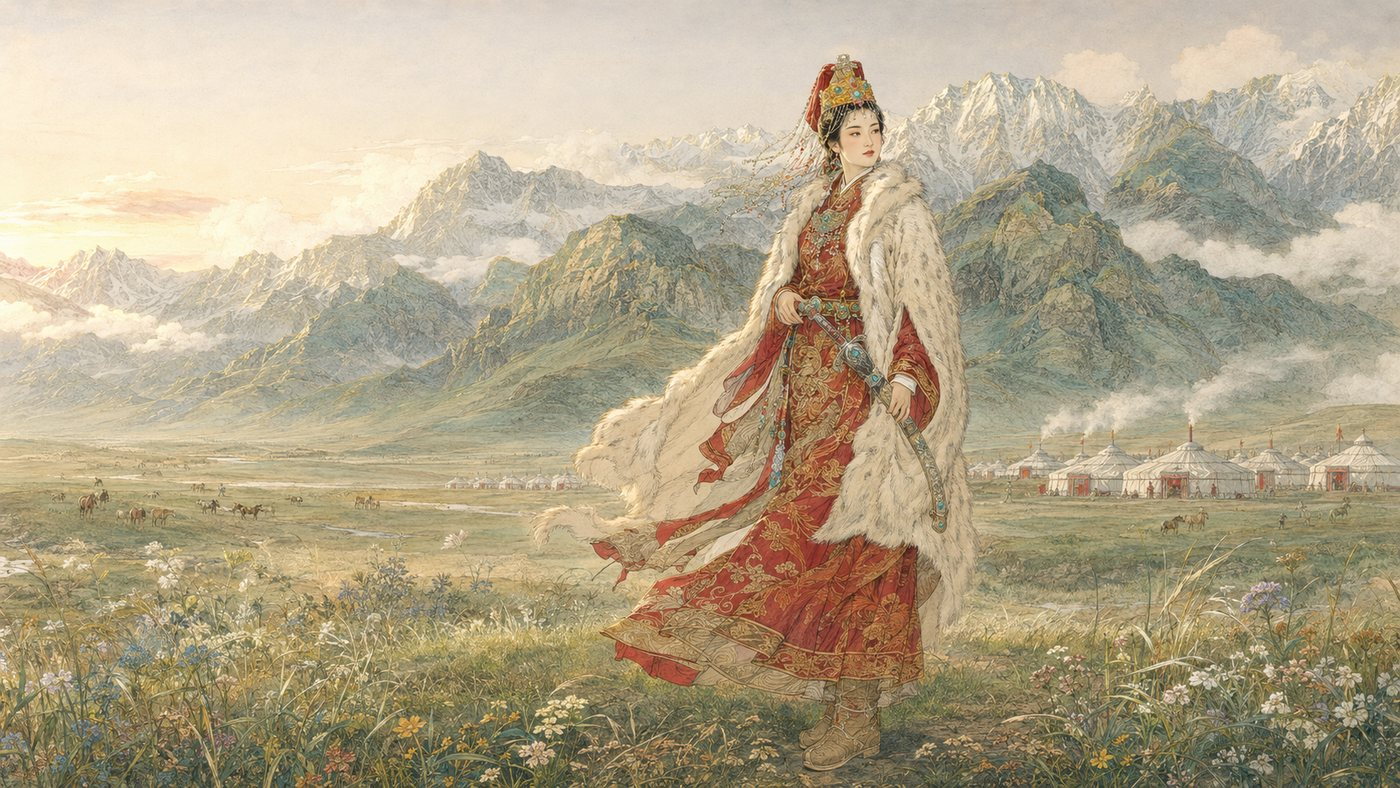
\includegraphics[width=0.92\linewidth,height=0.62\textheight,keepaspectratio]{assets/characters/zhaomin/portrait_01.jpg}
  \caption{赵敏第1拍《绿柳初逢》人物图。绿柳初逢。春柳、白貂与含而不露的笑意共同确立人物的机敏；冷白衣色与新绿背景相互映照，形成初见时的清锐感。}
  \label{fig:portrait:zhaomin:1}
\end{figure}

\Needspace{0.72\textheight}
\begin{figure}[H]
  \centering
  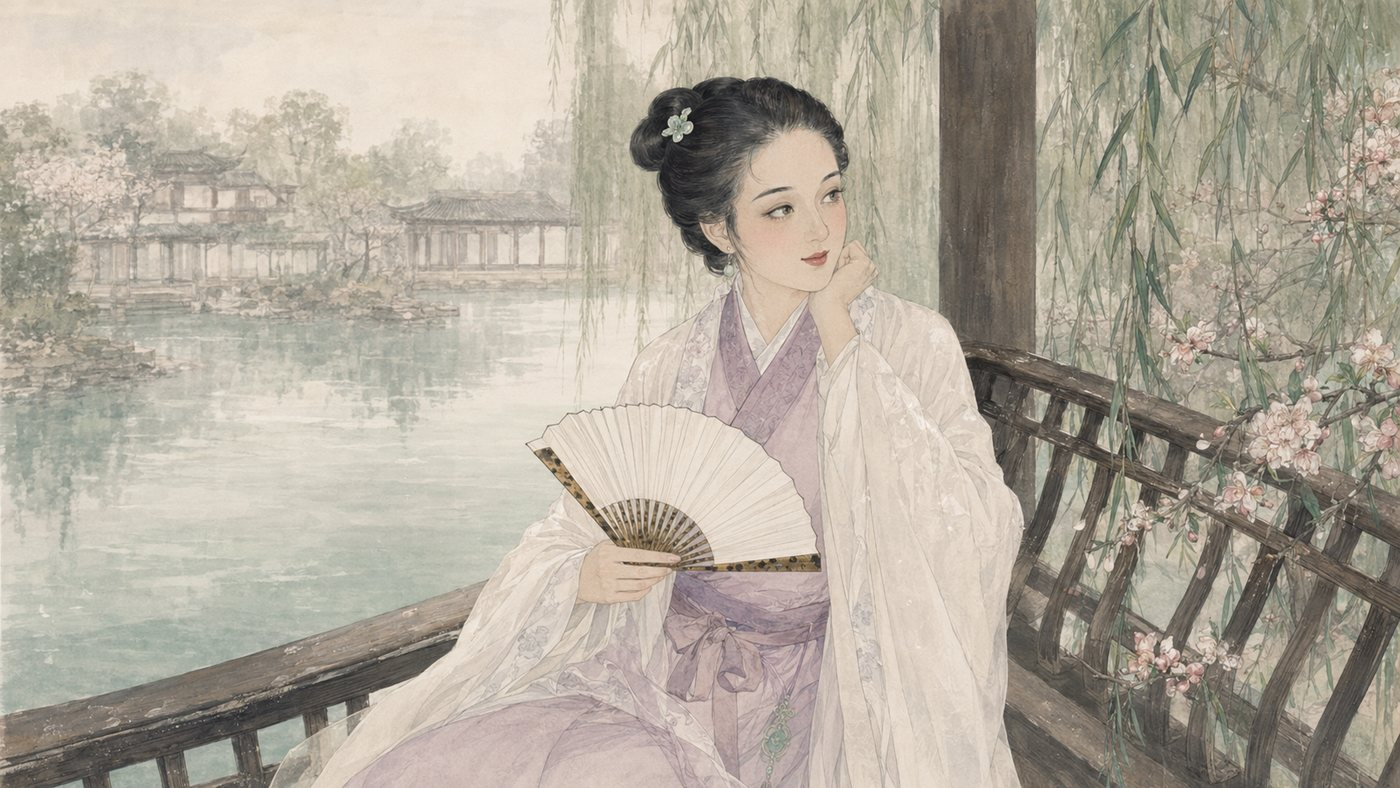
\includegraphics[width=0.92\linewidth,height=0.62\textheight,keepaspectratio]{assets/characters/zhaomin/portrait_02.jpg}
  \caption{赵敏第2拍《黑玉断续》人物图。黑玉断续。药物与伤体被置于同一视域，修复既是医理线索，也是关系重新建立的隐喻；暗色背景使人物的判断力成为视觉中心。}
  \label{fig:portrait:zhaomin:2}
\end{figure}

\Needspace{0.72\textheight}
\begin{figure}[H]
  \centering
  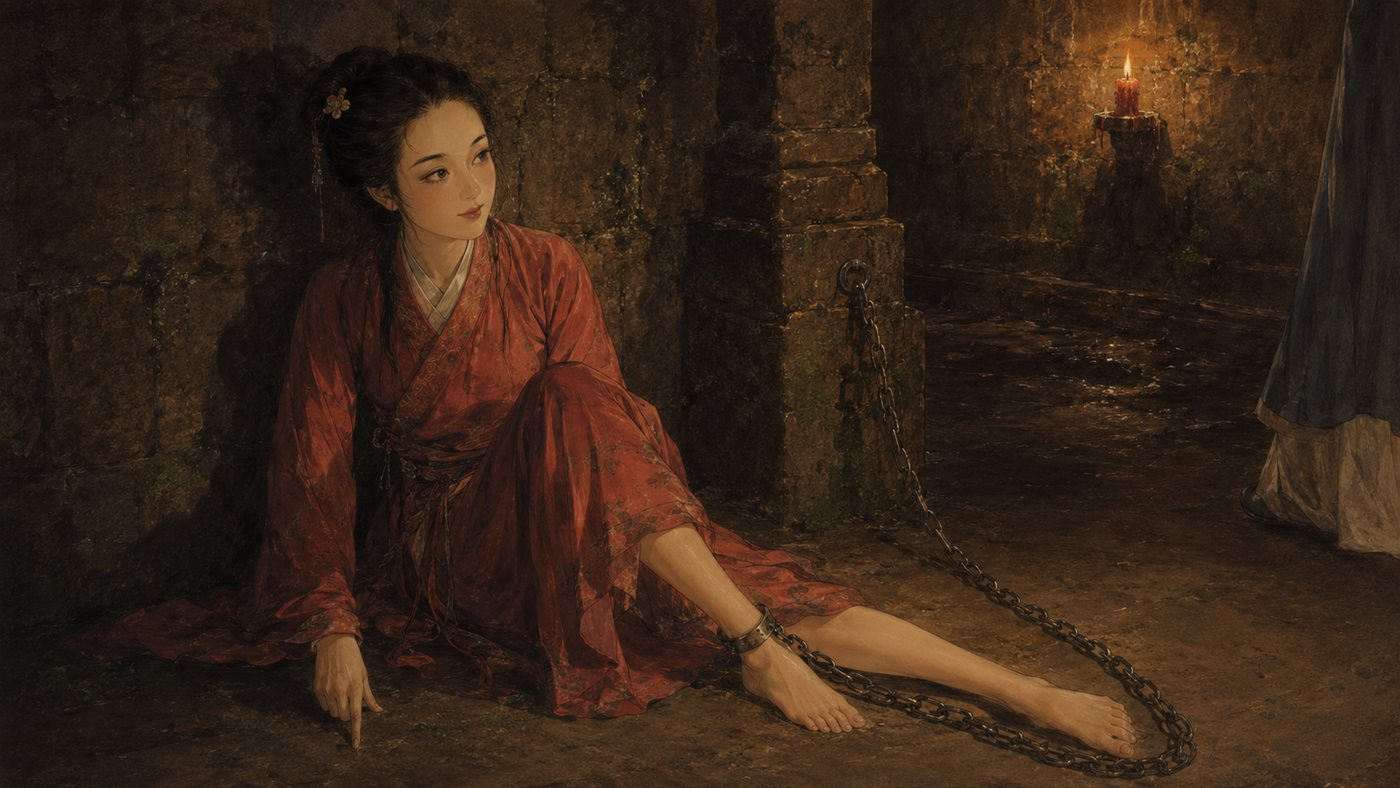
\includegraphics[width=0.92\linewidth,height=0.62\textheight,keepaspectratio]{assets/characters/zhaomin/portrait_03.jpg}
  \caption{赵敏第3拍《万安寺火》人物图。万安寺火。火光映照出危局中的决断，人物不以柔弱姿态出现；暖红与墨黑的强烈对照强化行动伦理与救援主题。}
  \label{fig:portrait:zhaomin:3}
\end{figure}

\Needspace{0.72\textheight}
\begin{figure}[H]
  \centering
  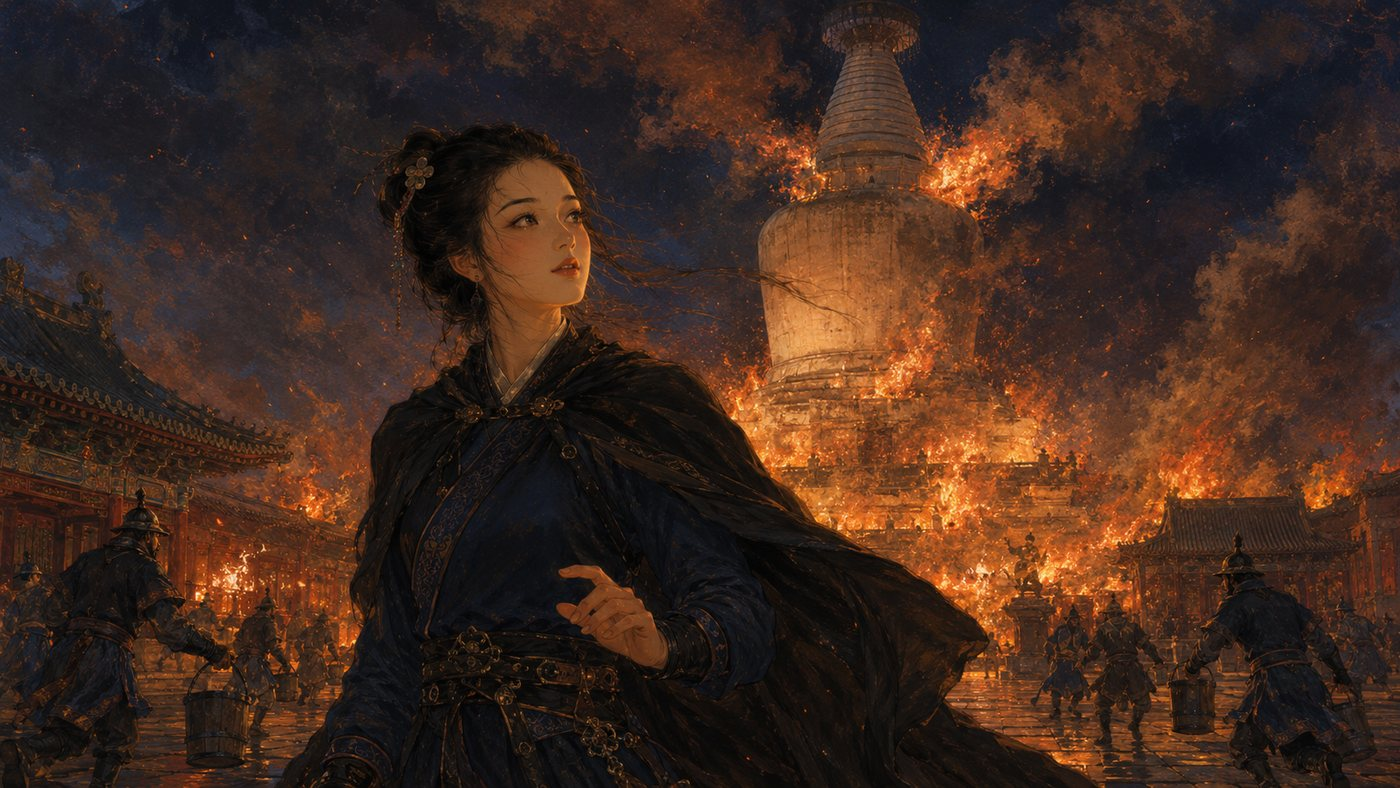
\includegraphics[width=0.92\linewidth,height=0.62\textheight,keepaspectratio]{assets/characters/zhaomin/portrait_04.jpg}
  \caption{赵敏第4拍《灵蛇海上》人物图。灵蛇海上。海雾、孤舟与远望构成漂泊感，暗示身份边界的松动；开阔留白使人物从权力中心暂时退入天地尺度。}
  \label{fig:portrait:zhaomin:4}
\end{figure}

\Needspace{0.72\textheight}
\begin{figure}[H]
  \centering
  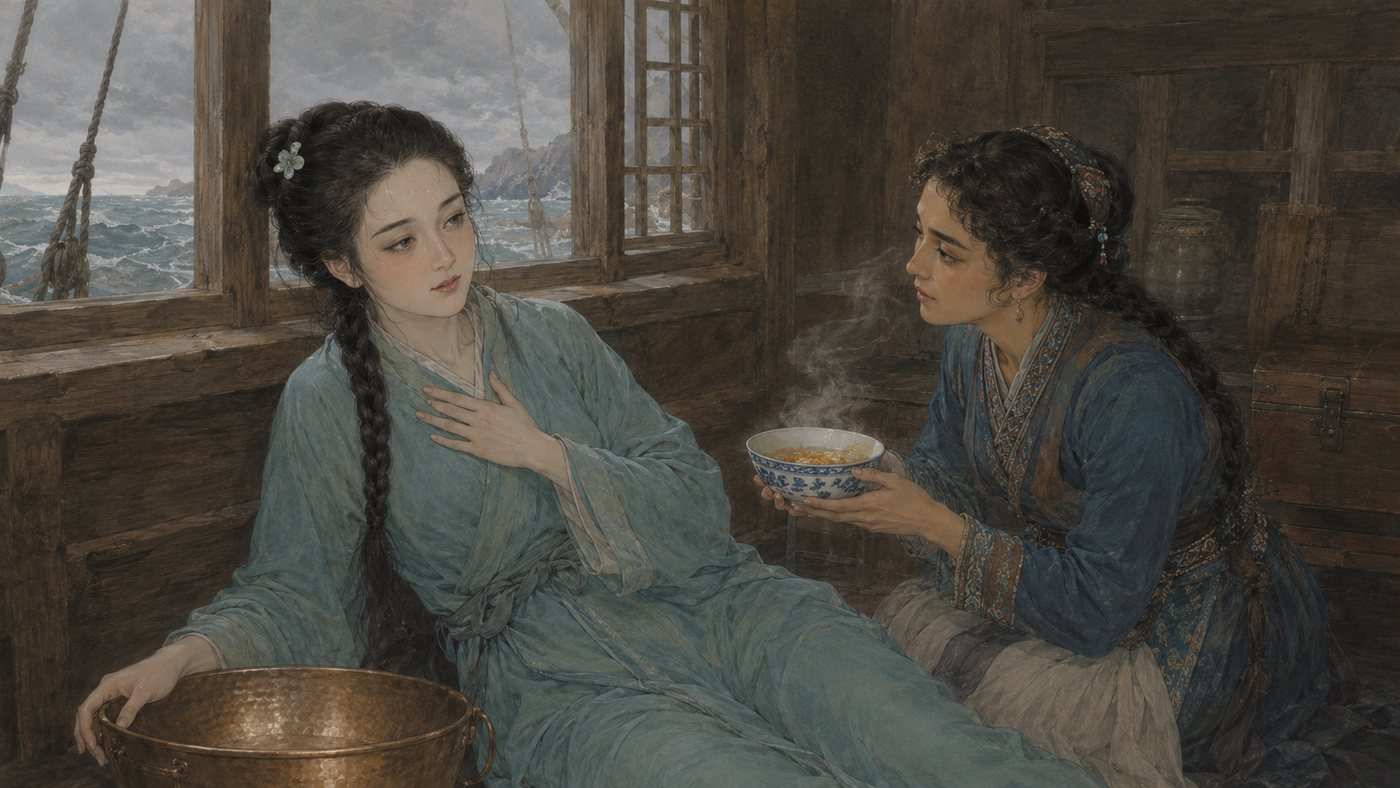
\includegraphics[width=0.92\linewidth,height=0.62\textheight,keepaspectratio]{assets/characters/zhaomin/portrait_05.jpg}
  \caption{赵敏第5拍《弥勒佛庙》人物图。弥勒佛庙。封闭建筑与斜入天光形成审问式空间，表现智谋背后的风险；构图以明暗分界提示真相并非全然可见。}
  \label{fig:portrait:zhaomin:5}
\end{figure}

\Needspace{0.72\textheight}
\begin{figure}[H]
  \centering
  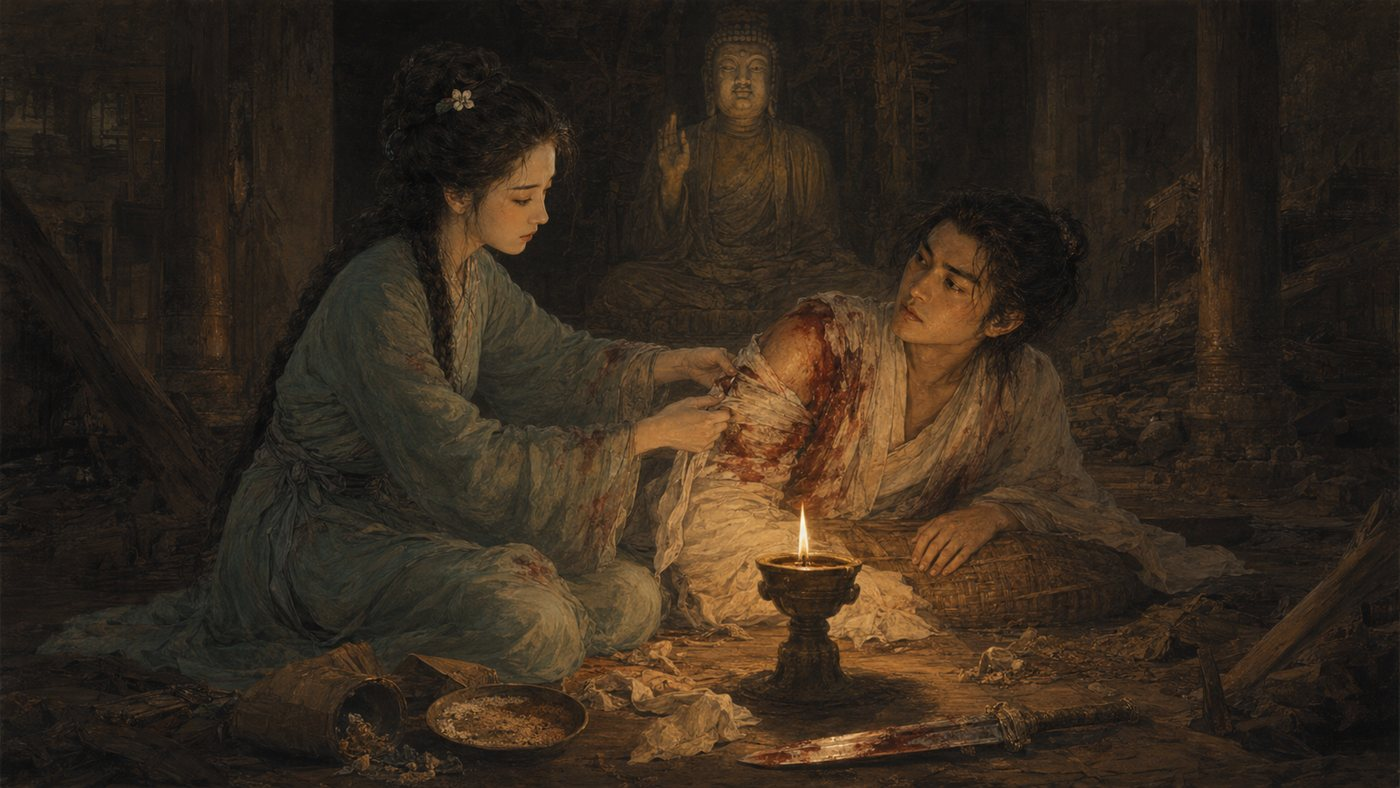
\includegraphics[width=0.92\linewidth,height=0.62\textheight,keepaspectratio]{assets/characters/zhaomin/portrait_06.jpg}
  \caption{赵敏第6拍《濠州夺婚》人物图。濠州夺婚。红色礼制空间被人物的侧身动作打破，象征个人选择对既定秩序的冲撞；高饱和朱红集中呈现情感张力。}
  \label{fig:portrait:zhaomin:6}
\end{figure}

\Needspace{0.72\textheight}
\begin{figure}[H]
  \centering
  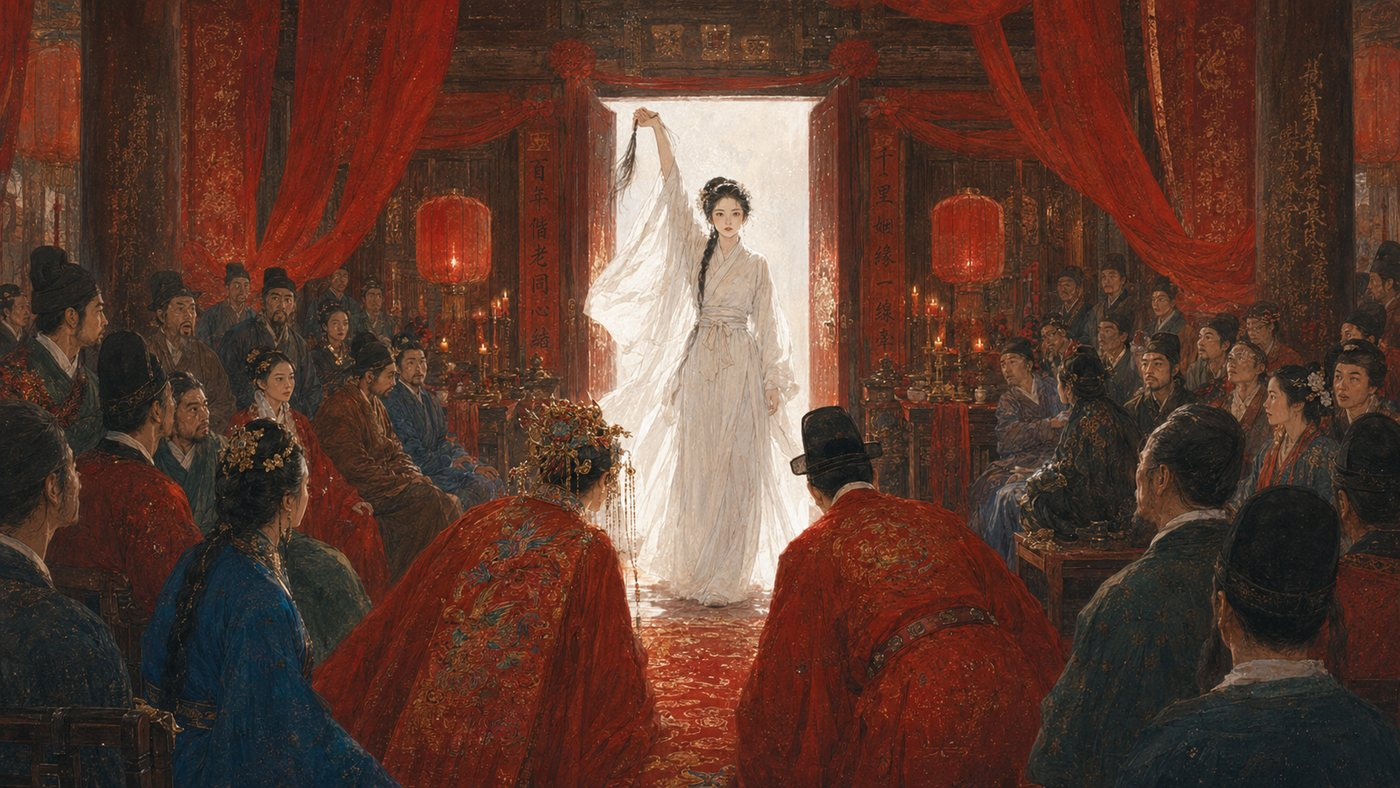
\includegraphics[width=0.92\linewidth,height=0.62\textheight,keepaspectratio]{assets/characters/zhaomin/portrait_07.jpg}
  \caption{赵敏第7拍《少室山下》人物图。少室山下。山门与石阶强调制度和传统的重量，人物的稳定站姿则保留自主意志；纵深透视使选择具有路径感。}
  \label{fig:portrait:zhaomin:7}
\end{figure}

\Needspace{0.72\textheight}
\begin{figure}[H]
  \centering
  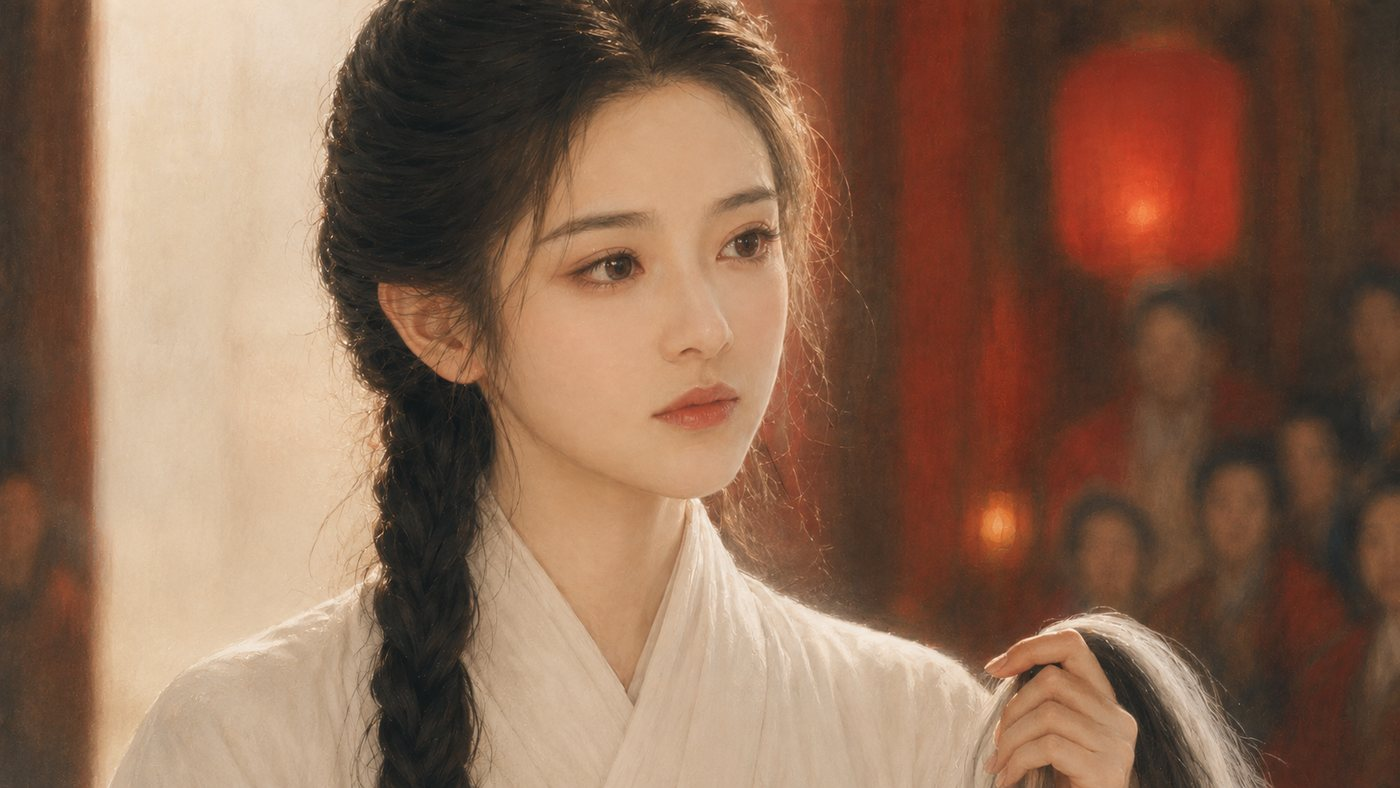
\includegraphics[width=0.92\linewidth,height=0.62\textheight,keepaspectratio]{assets/characters/zhaomin/portrait_08.jpg}
  \caption{赵敏第8拍《朔漠风霜》人物图。朔漠风霜。风沙削弱华饰，凸显身体对环境的真实承受；赭石与灰蓝构成冷暖错位，表现坚韧并非没有代价。}
  \label{fig:portrait:zhaomin:8}
\end{figure}

\Needspace{0.72\textheight}
\begin{figure}[H]
  \centering
  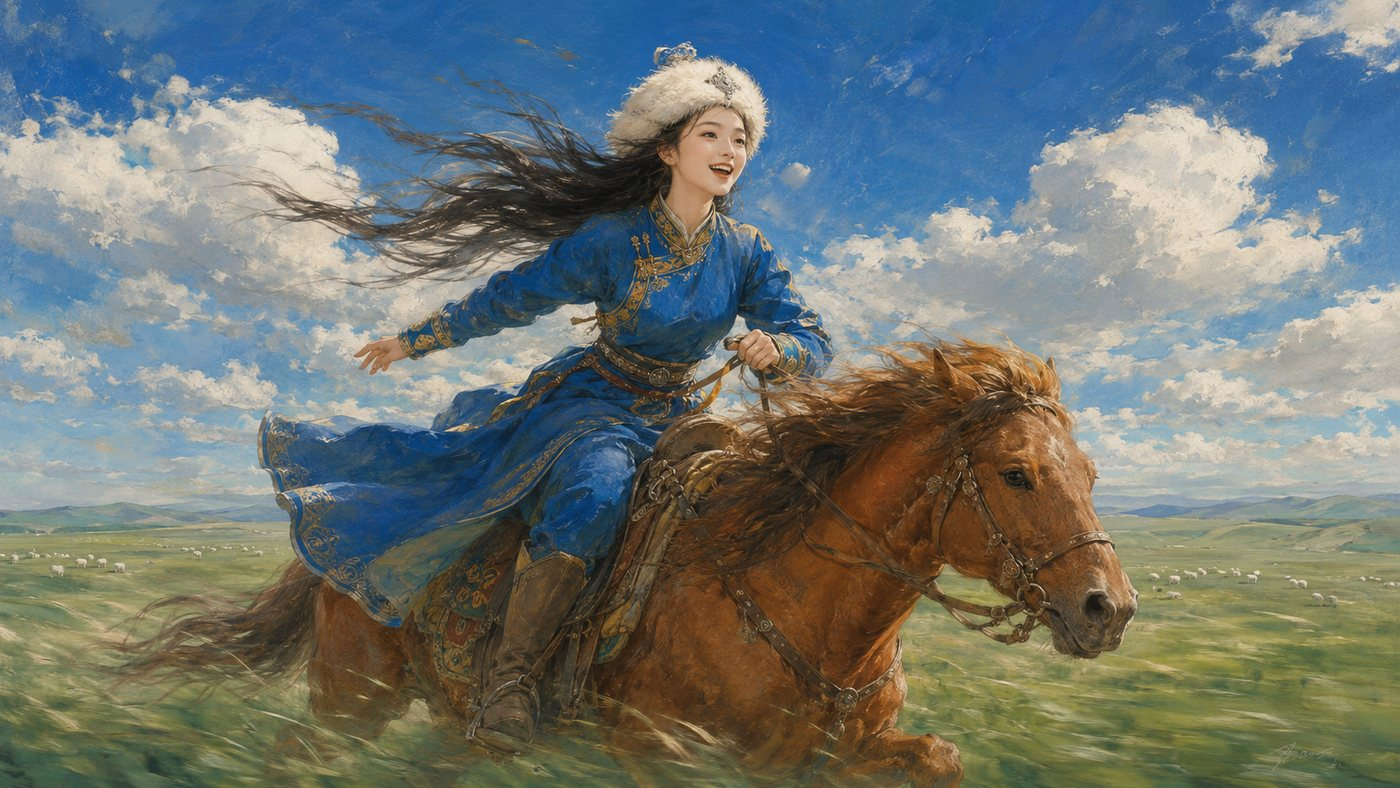
\includegraphics[width=0.92\linewidth,height=0.62\textheight,keepaspectratio]{assets/characters/zhaomin/portrait_09.jpg}
  \caption{赵敏第9拍《冰火之岛》人物图。冰火之岛。极寒与火山并置，象征生命处境中的冲突和调和；人物位于两种光源之间，成为平衡而非征服自然的主体。}
  \label{fig:portrait:zhaomin:9}
\end{figure}

\Needspace{0.72\textheight}
\begin{figure}[H]
  \centering
  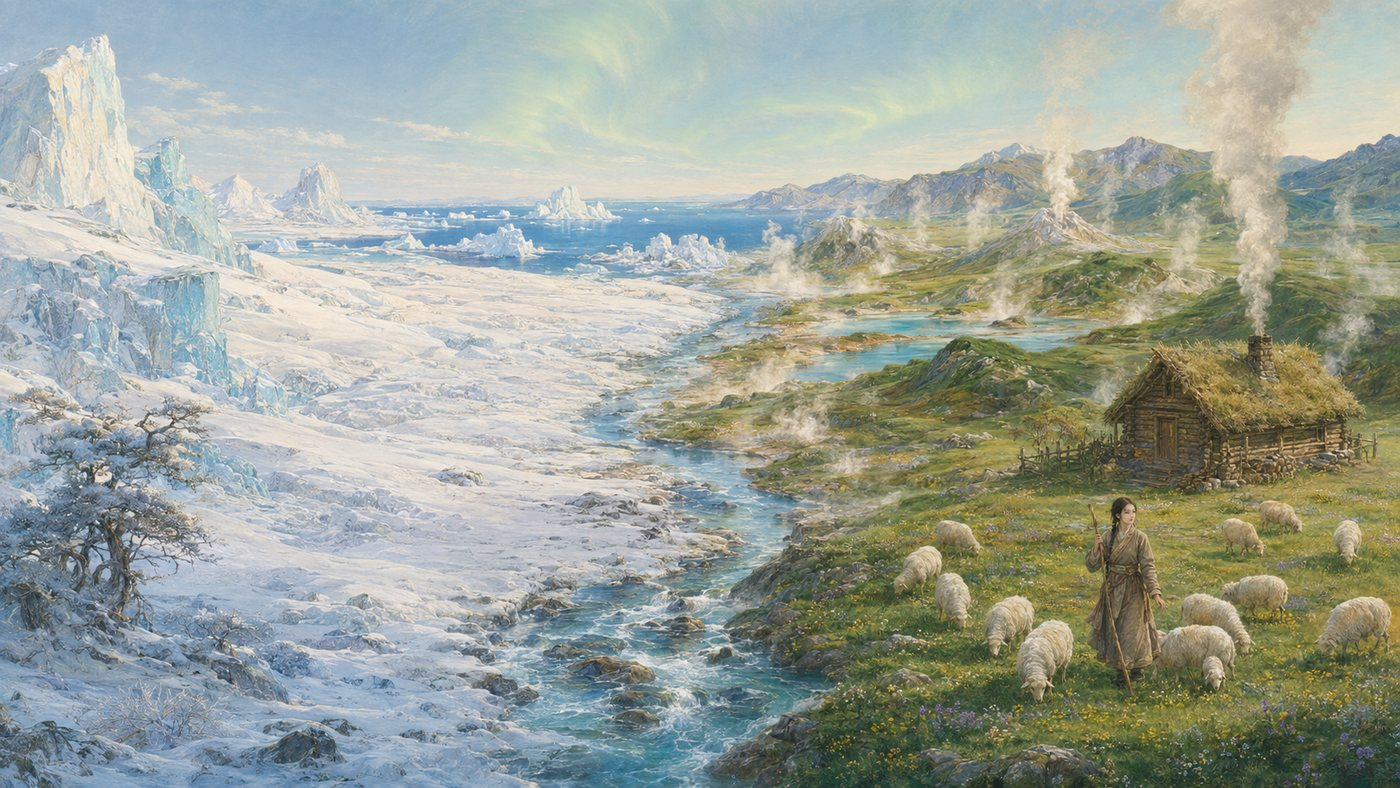
\includegraphics[width=0.92\linewidth,height=0.62\textheight,keepaspectratio]{assets/characters/zhaomin/portrait_10.jpg}
  \caption{赵敏第10拍《父女恩仇》人物图。父女恩仇。宫廷秩序与亲缘裂隙同时进入画面，人物表情克制，避免将伦理冲突处理为单一善恶；对称构图有意制造压迫感。}
  \label{fig:portrait:zhaomin:10}
\end{figure}

\Needspace{0.72\textheight}
\begin{figure}[H]
  \centering
  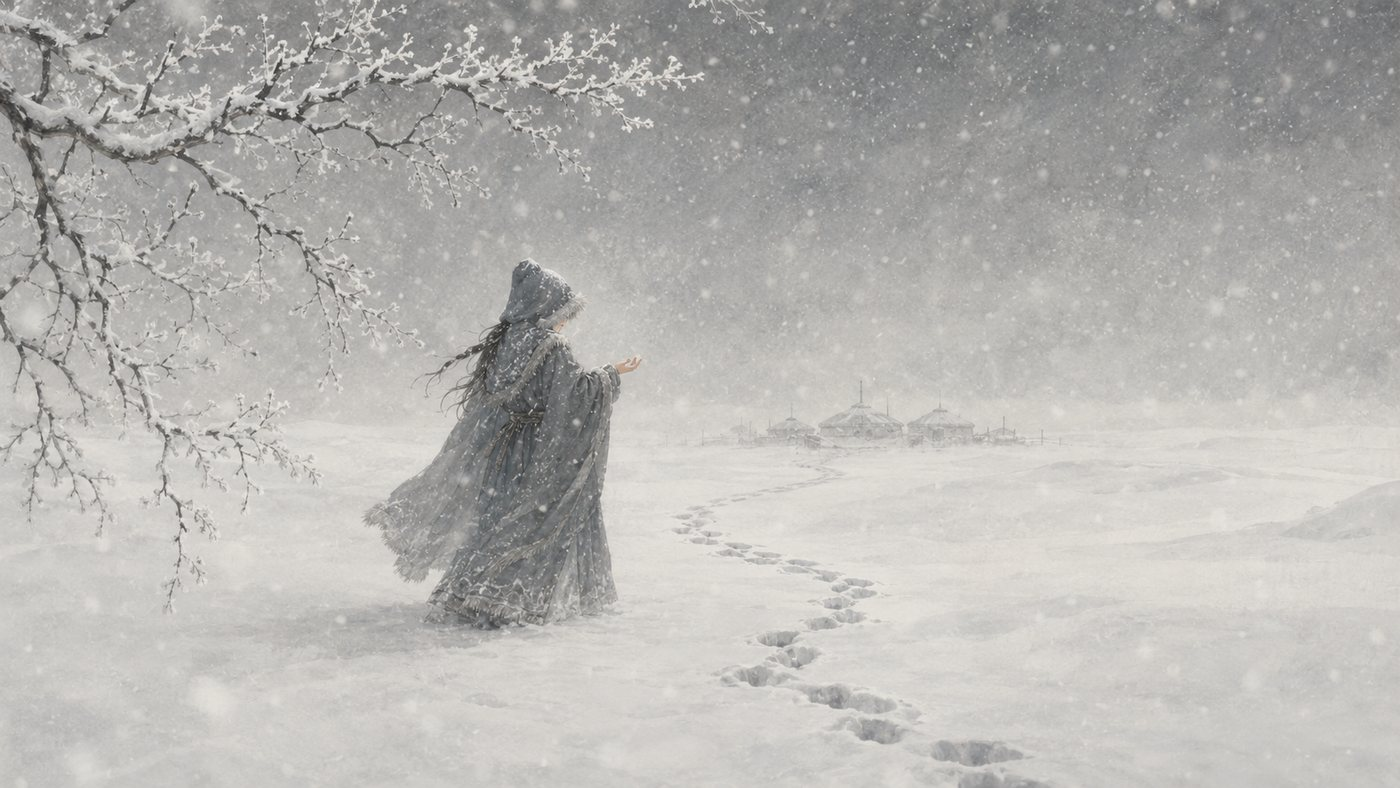
\includegraphics[width=0.92\linewidth,height=0.62\textheight,keepaspectratio]{assets/characters/zhaomin/portrait_11.jpg}
  \caption{赵敏第11拍《玄冥寒掌》人物图。玄冥寒掌。冷色侵入肤色，提示疾病与创伤首先发生于身体；局部暖光保留康复可能，使痛苦不被审美化。}
  \label{fig:portrait:zhaomin:11}
\end{figure}

\Needspace{0.72\textheight}
\begin{figure}[H]
  \centering
  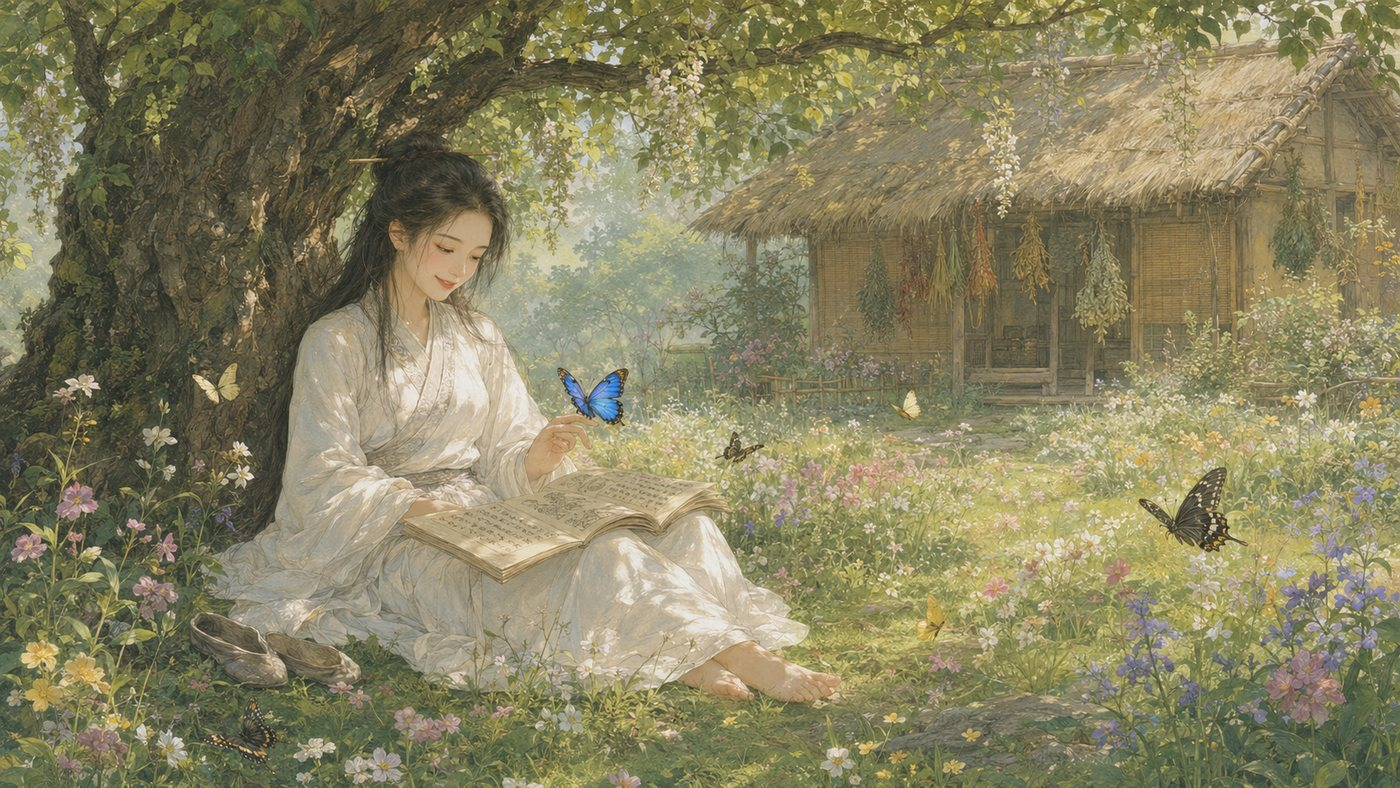
\includegraphics[width=0.92\linewidth,height=0.62\textheight,keepaspectratio]{assets/characters/zhaomin/portrait_12.jpg}
  \caption{赵敏第12拍《大都宫闱》人物图。大都宫闱。高墙、帷幕与狭窄天光表现权力空间的规训，人物目光越出画面，暗示精神上的出走。}
  \label{fig:portrait:zhaomin:12}
\end{figure}

\Needspace{0.72\textheight}
\begin{figure}[H]
  \centering
  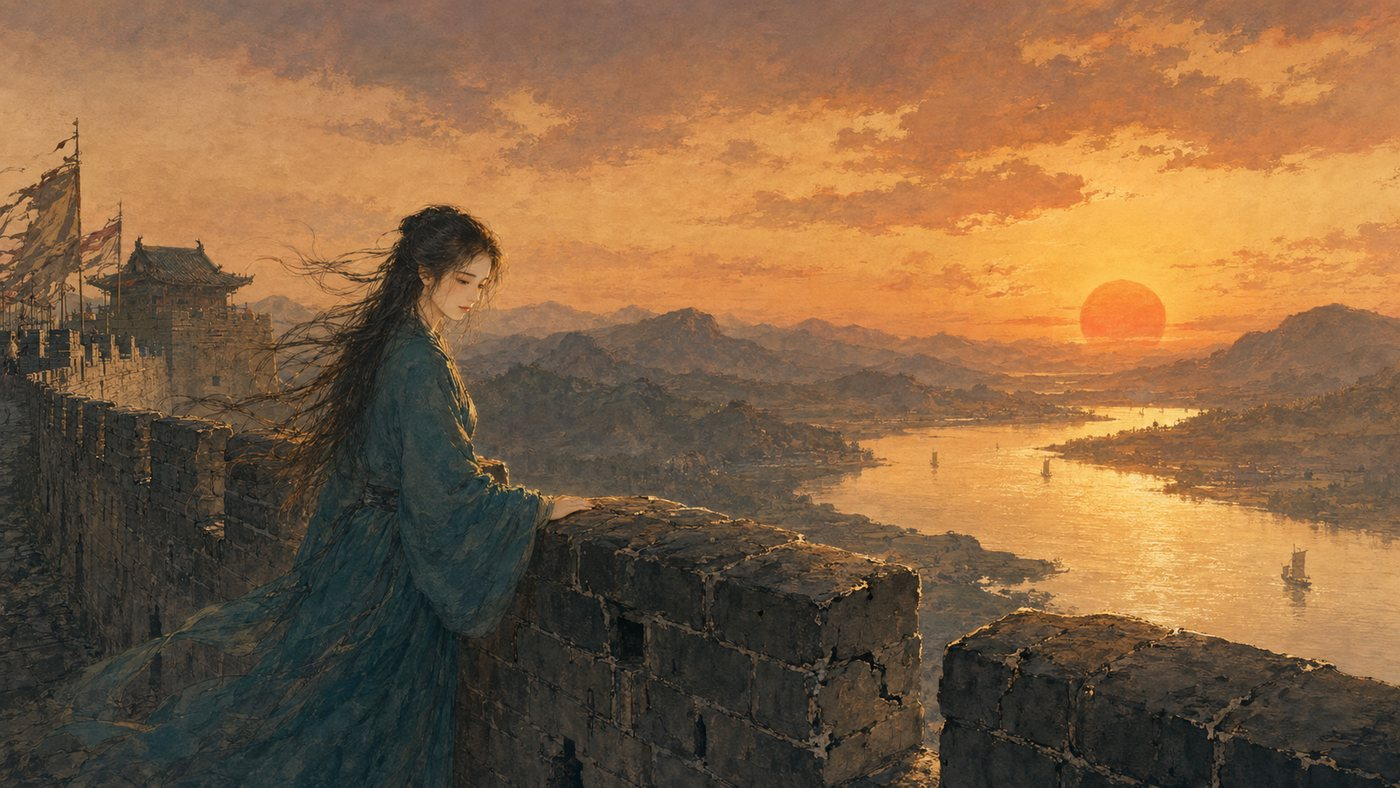
\includegraphics[width=0.92\linewidth,height=0.62\textheight,keepaspectratio]{assets/characters/zhaomin/portrait_13.jpg}
  \caption{赵敏第13拍《蝴蝶谷中》人物图。蝴蝶谷中。草木、药圃与缓和光线将照护置于日常劳动中；绿色层次表现医学知识与自然观察之间的联系。}
  \label{fig:portrait:zhaomin:13}
\end{figure}

\Needspace{0.72\textheight}
\begin{figure}[H]
  \centering
  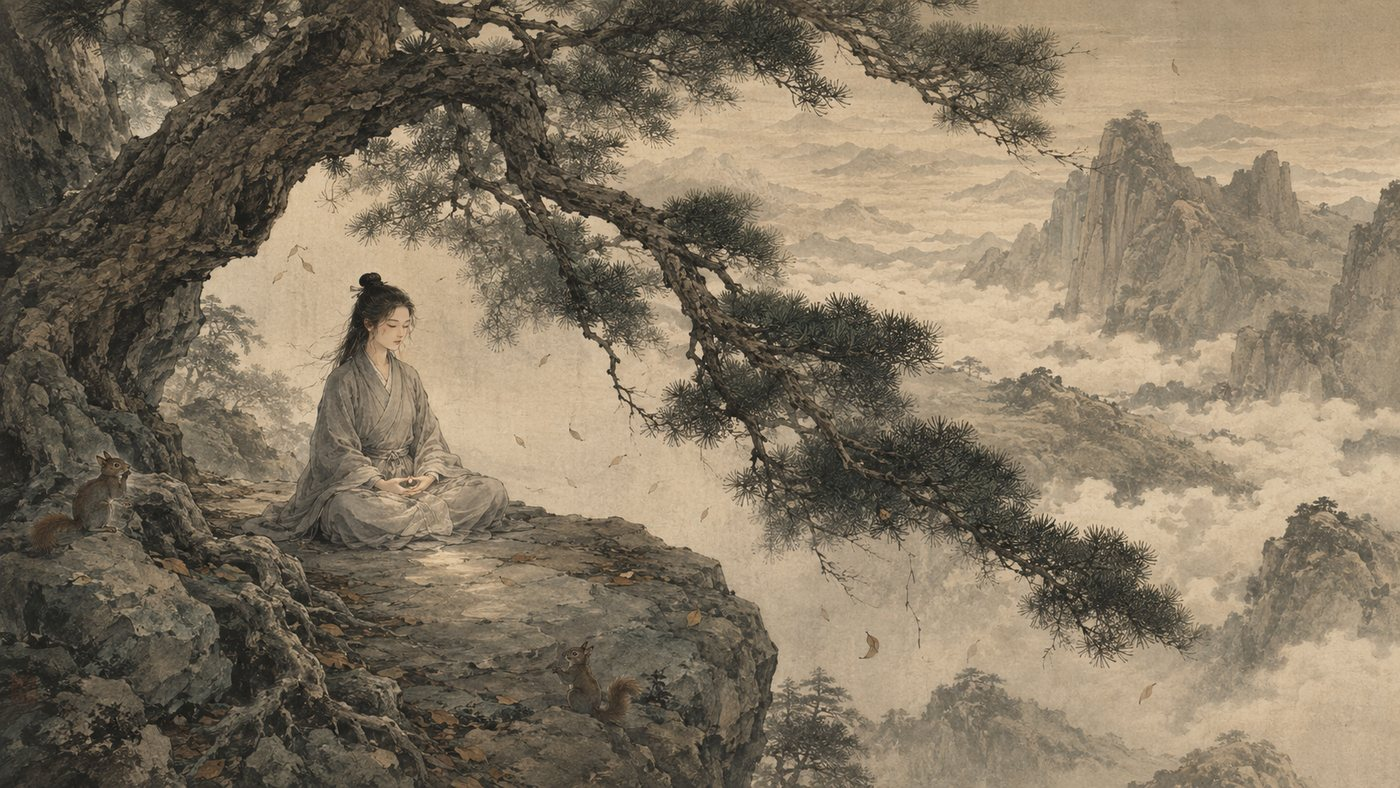
\includegraphics[width=0.92\linewidth,height=0.62\textheight,keepaspectratio]{assets/characters/zhaomin/portrait_14.jpg}
  \caption{赵敏第14拍《光明顶上》人物图。光明顶上。高山风云扩大人物行动的公共尺度，衣袂与云势同向，形成介入历史的动感；留白避免英雄化过度。}
  \label{fig:portrait:zhaomin:14}
\end{figure}

\Needspace{0.72\textheight}
\begin{figure}[H]
  \centering
  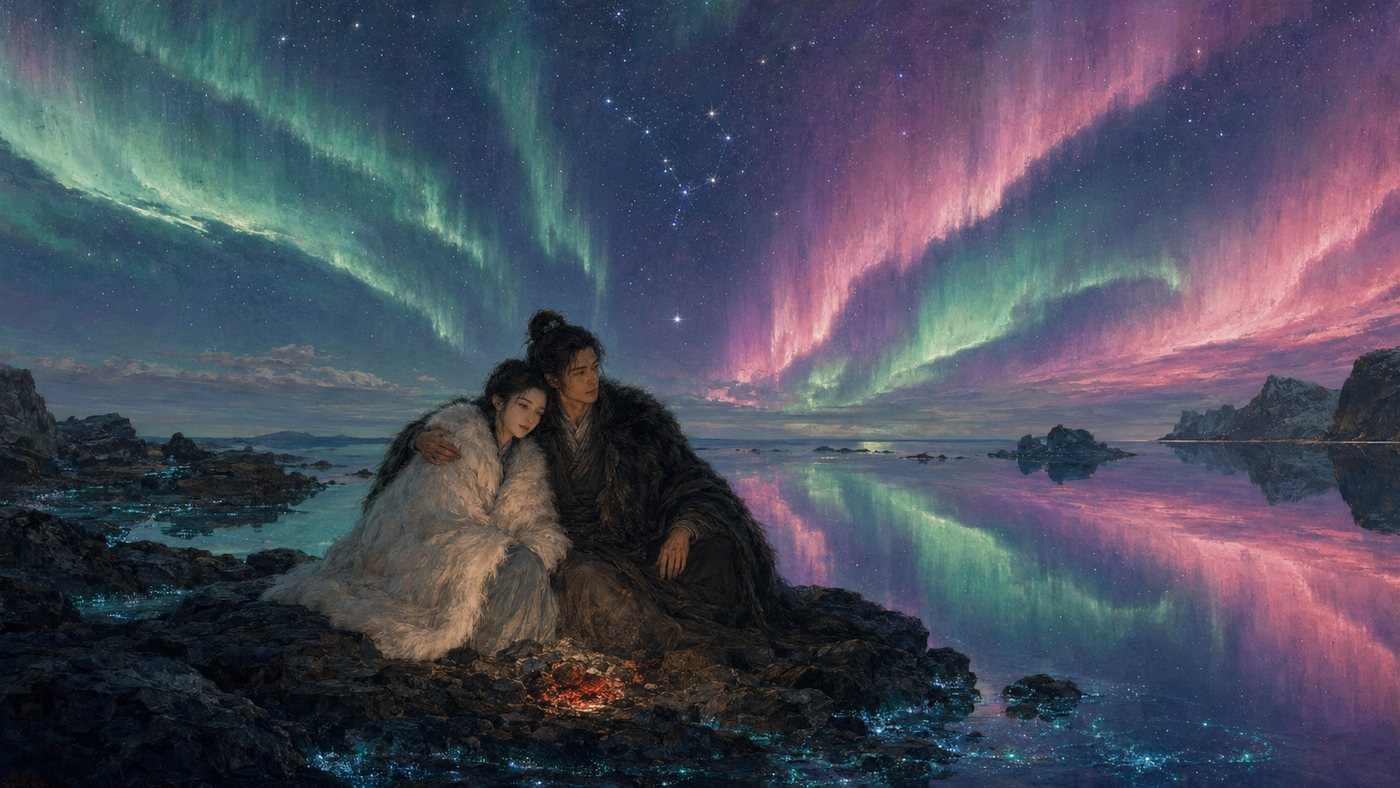
\includegraphics[width=0.92\linewidth,height=0.62\textheight,keepaspectratio]{assets/characters/zhaomin/portrait_15.jpg}
  \caption{赵敏第15拍《波斯异术》人物图。波斯异术。异域纹样与中原服饰并置，表现跨文化知识相遇；色彩差异被组织为互补关系，而非奇观化装饰。}
  \label{fig:portrait:zhaomin:15}
\end{figure}

\Needspace{0.72\textheight}
\begin{figure}[H]
  \centering
  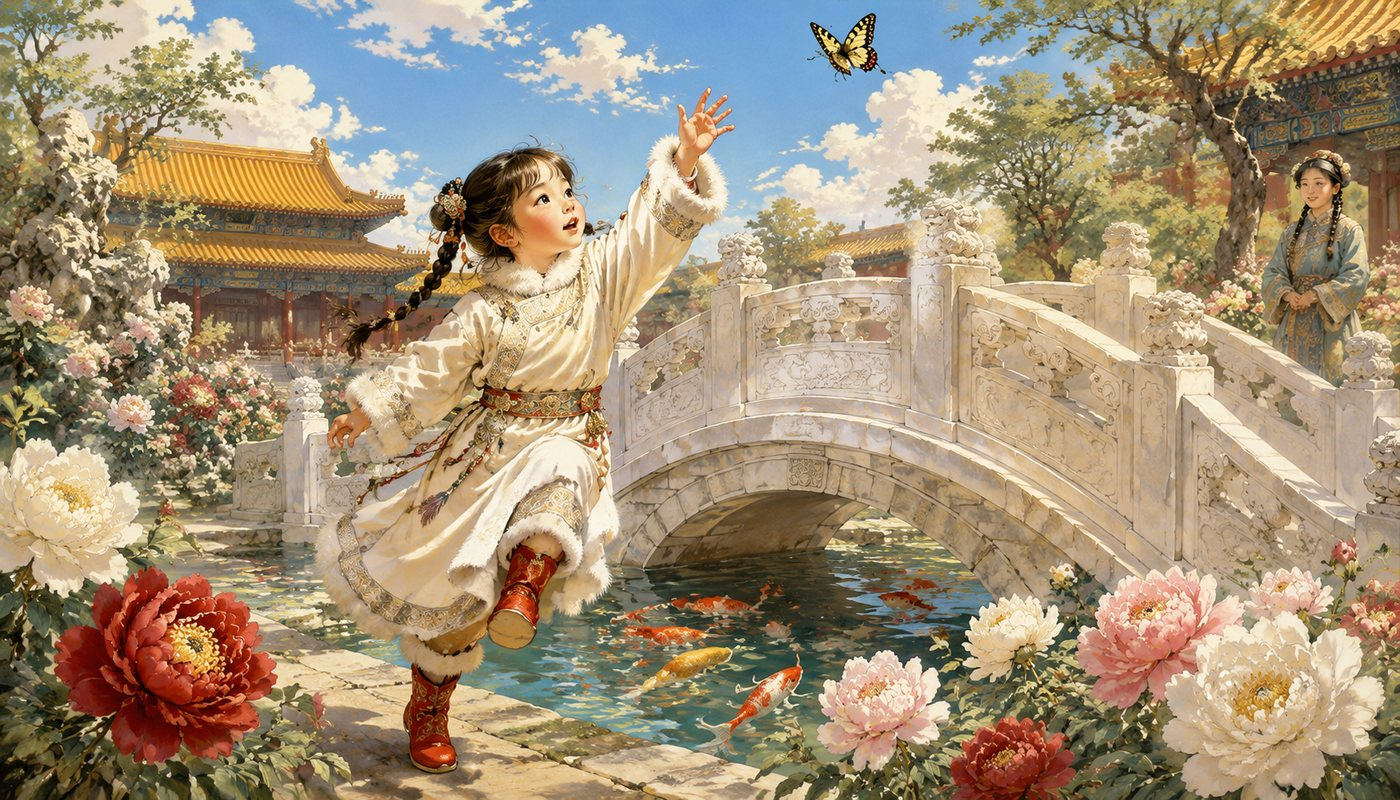
\includegraphics[width=0.92\linewidth,height=0.62\textheight,keepaspectratio]{assets/characters/zhaomin/portrait_16.jpg}
  \caption{赵敏第16拍《襄阳遗梦》人物图。襄阳遗梦。城墙、暮色与远方烽烟构成历史记忆，人物不再处于战斗中心；低饱和色调强调反思多于胜负。}
  \label{fig:portrait:zhaomin:16}
\end{figure}

\Needspace{0.72\textheight}
\begin{figure}[H]
  \centering
  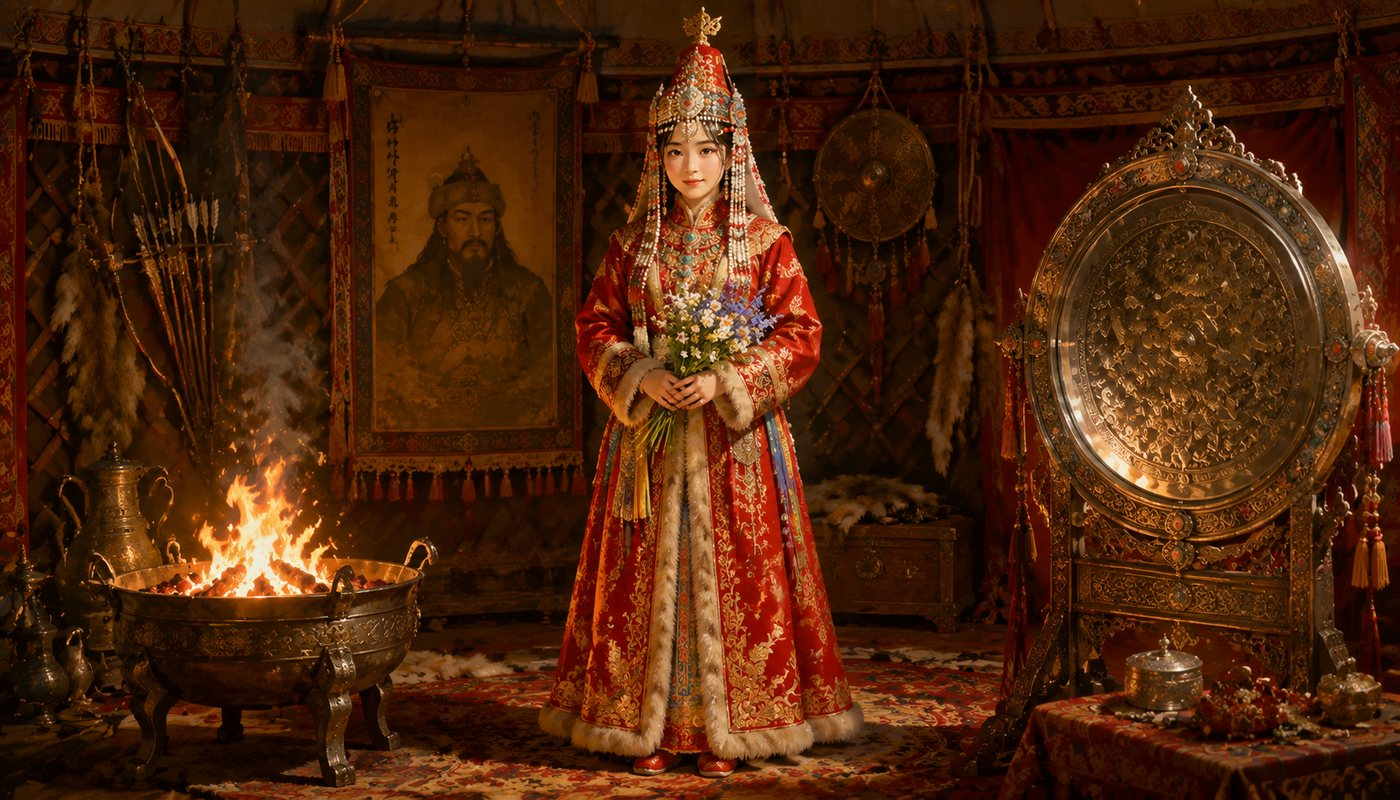
\includegraphics[width=0.92\linewidth,height=0.62\textheight,keepaspectratio]{assets/characters/zhaomin/portrait_17.jpg}
  \caption{赵敏第17拍《终南问道》人物图。终南问道。山径与云雾指向向内的追问，简化服饰和道具，削弱郡主身份；画面以清淡墨色表现精神减负。}
  \label{fig:portrait:zhaomin:17}
\end{figure}

\Needspace{0.72\textheight}
\begin{figure}[H]
  \centering
  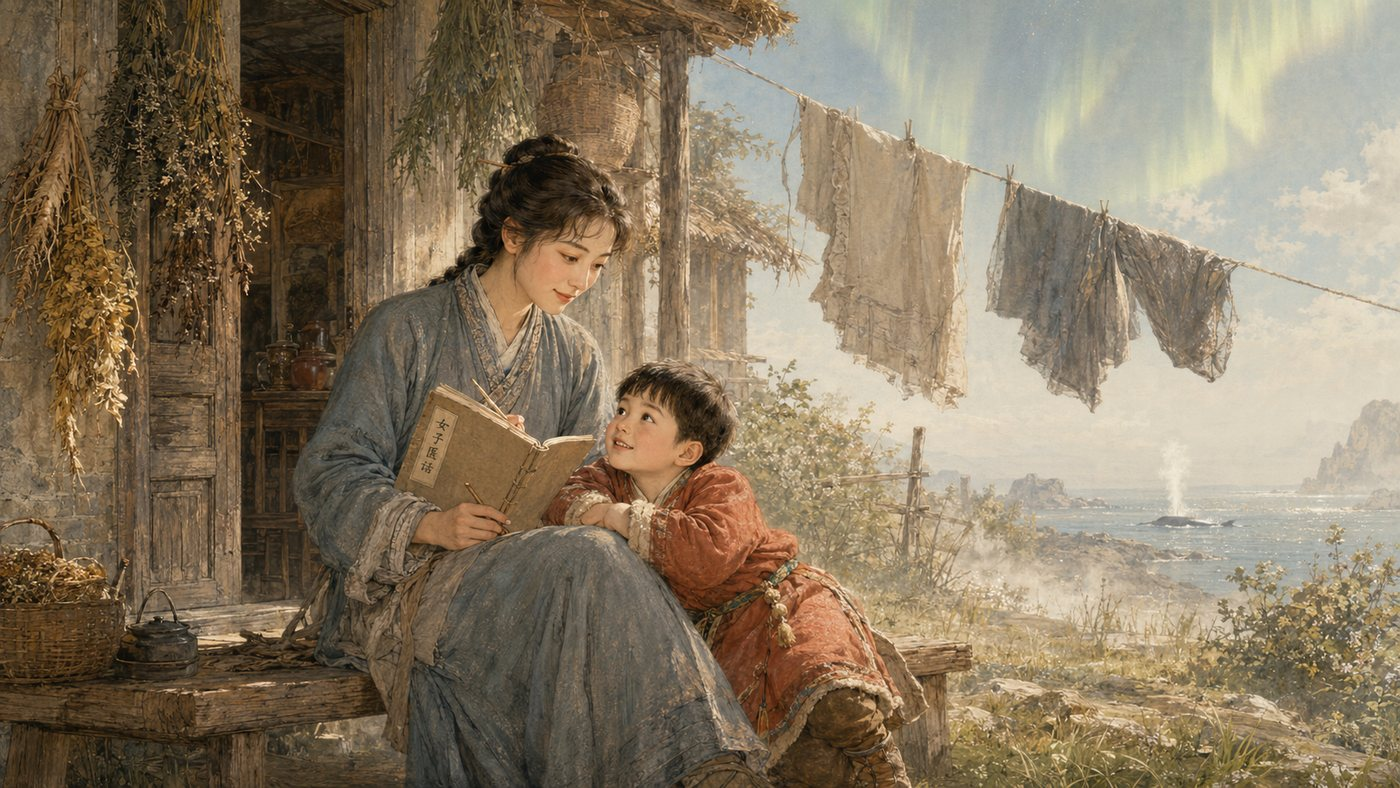
\includegraphics[width=0.92\linewidth,height=0.62\textheight,keepaspectratio]{assets/characters/zhaomin/portrait_18.jpg}
  \caption{赵敏第18拍《天下归心》人物图。天下归心。广阔天际与安定人间取代宫廷权力，人物神态平和；暖金色被控制在边缘光中，表达愿望而非凯旋。}
  \label{fig:portrait:zhaomin:18}
\end{figure}

\subsubsection{周芷若人物图录}

\Needspace{0.72\textheight}
\begin{figure}[H]
  \centering
  
\includegraphics[width=0.92\linewidth,height=0.62\textheight,keepaspectratio]{assets/characters/zhouzhiruo/portrait_01.jpg}
  \caption{周芷若第1拍《汉水初遇》人物图。汉水初遇。水岸、薄雾与少女形象建立生命早期的脆弱和澄明；低视点使人物与江流处于同一命运尺度。}
  \label{fig:portrait:zhouzhiruo:1}
\end{figure}

\Needspace{0.72\textheight}
\begin{figure}[H]
  \centering
  
\includegraphics[width=0.92\linewidth,height=0.62\textheight,keepaspectratio]{assets/characters/zhouzhiruo/portrait_02.jpg}
  \caption{周芷若第2拍《峨眉入门》人物图。峨眉入门。山门与规整石阶表现师门秩序，人物居于纵深入口，暗示成长始于接受也始于约束。}
  \label{fig:portrait:zhouzhiruo:2}
\end{figure}

\Needspace{0.72\textheight}
\begin{figure}[H]
  \centering
  
\includegraphics[width=0.92\linewidth,height=0.62\textheight,keepaspectratio]{assets/characters/zhouzhiruo/portrait_03.jpg}
  \caption{周芷若第3拍《光明一剑》人物图。光明一剑。剑势切开静态构图，表现命令、情感与身体动作之间的冲突；冷光强调决断所带来的创伤。}
  \label{fig:portrait:zhouzhiruo:3}
\end{figure}

\Needspace{0.72\textheight}
\begin{figure}[H]
  \centering
  
\includegraphics[width=0.92\linewidth,height=0.62\textheight,keepaspectratio]{assets/characters/zhouzhiruo/portrait_04.jpg}
  \caption{周芷若第4拍《万安寺誓》人物图。万安寺誓。高塔、夜色与微弱灯火构成封闭环境，人物姿态克制；竖向结构强化誓言的重量和不可退避感。}
  \label{fig:portrait:zhouzhiruo:4}
\end{figure}

\Needspace{0.72\textheight}
\begin{figure}[H]
  \centering
  
\includegraphics[width=0.92\linewidth,height=0.62\textheight,keepaspectratio]{assets/characters/zhouzhiruo/portrait_05.jpg}
  \caption{周芷若第5拍《灵蛇毒计》人物图。灵蛇毒计。海岛雾气遮蔽空间关系，象征猜疑与误认；人物与危险物之间保留距离，使伦理警觉先于戏剧刺激。}
  \label{fig:portrait:zhouzhiruo:5}
\end{figure}

\Needspace{0.72\textheight}
\begin{figure}[H]
  \centering
  
\includegraphics[width=0.92\linewidth,height=0.62\textheight,keepaspectratio]{assets/characters/zhouzhiruo/portrait_06.jpg}
  \caption{周芷若第6拍《裂裳之痛》人物图。裂裳之痛。破损衣料作为创伤痕迹而非猎奇细节，画面压低色彩与动作幅度，维护人物尊严。}
  \label{fig:portrait:zhouzhiruo:6}
\end{figure}

\Needspace{0.72\textheight}
\begin{figure}[H]
  \centering
  
\includegraphics[width=0.92\linewidth,height=0.62\textheight,keepaspectratio]{assets/characters/zhouzhiruo/portrait_07.jpg}
  \caption{周芷若第7拍《九阴白骨》人物图。九阴白骨。强烈墨色和骨白形成近乎失衡的视觉张力，表现力量对主体的反噬；边缘留白保存自我回返的可能。}
  \label{fig:portrait:zhouzhiruo:7}
\end{figure}

\Needspace{0.72\textheight}
\begin{figure}[H]
  \centering
  
\includegraphics[width=0.92\linewidth,height=0.62\textheight,keepaspectratio]{assets/characters/zhouzhiruo/portrait_08.jpg}
  \caption{周芷若第8拍《峨眉掌门》人物图。峨眉掌门。正面构图与门派器物呈现制度身份，人物目光略偏离中轴，提示权威与内心并未完全重合。}
  \label{fig:portrait:zhouzhiruo:8}
\end{figure}

\Needspace{0.72\textheight}
\begin{figure}[H]
  \centering
  
\includegraphics[width=0.92\linewidth,height=0.62\textheight,keepaspectratio]{assets/characters/zhouzhiruo/portrait_09.jpg}
  \caption{周芷若第9拍《屠狮之会》人物图。屠狮之会。群体空间被压缩为围合结构，表现公共审判的压力；人物处于视觉焦点，却不被塑造成单纯胜者。}
  \label{fig:portrait:zhouzhiruo:9}
\end{figure}

\Needspace{0.72\textheight}
\begin{figure}[H]
  \centering
  
\includegraphics[width=0.92\linewidth,height=0.62\textheight,keepaspectratio]{assets/characters/zhouzhiruo/portrait_10.jpg}
  \caption{周芷若第10拍《黄衫女子》人物图。黄衫女子。明黄与素白的相遇形成镜像关系，象征另一种女性力量介入；双主体构图避免把比较化为高下评判。}
  \label{fig:portrait:zhouzhiruo:10}
\end{figure}

\Needspace{0.72\textheight}
\begin{figure}[H]
  \centering
  
\includegraphics[width=0.92\linewidth,height=0.62\textheight,keepaspectratio]{assets/characters/zhouzhiruo/portrait_11.jpg}
  \caption{周芷若第11拍《问心有愧》人物图。问心有愧。空室、灯影与低垂视线将冲突转向内在，画面减少道具，让悔悟成为持续的伦理劳动。}
  \label{fig:portrait:zhouzhiruo:11}
\end{figure}

\Needspace{0.72\textheight}
\begin{figure}[H]
  \centering
  
\includegraphics[width=0.92\linewidth,height=0.62\textheight,keepaspectratio]{assets/characters/zhouzhiruo/portrait_12.jpg}
  \caption{周芷若第12拍《汉水归舟》人物图。汉水归舟。归舟重返最初的水域意象，江面留白承接记忆与宽恕；人物背影弱化身份标签，突出返身自省。}
  \label{fig:portrait:zhouzhiruo:12}
\end{figure}

\Needspace{0.72\textheight}
\begin{figure}[H]
  \centering
  
\includegraphics[width=0.92\linewidth,height=0.62\textheight,keepaspectratio]{assets/characters/zhouzhiruo/portrait_13.jpg}
  \caption{周芷若第13拍《峨眉金顶》人物图。峨眉金顶。云海与金顶构成超越性背景，人物尺度被有意缩小；宏阔空间不再服务权威，而用于重新理解归属。}
  \label{fig:portrait:zhouzhiruo:13}
\end{figure}

\Needspace{0.72\textheight}
\begin{figure}[H]
  \centering
  
\includegraphics[width=0.92\linewidth,height=0.62\textheight,keepaspectratio]{assets/characters/zhouzhiruo/portrait_14.jpg}
  \caption{周芷若第14拍《药王谷中》人物图。药王谷中。药架、草木与书写活动表现知识由秘术转向公共照护；柔和自然光建立可学习、可传承的医学氛围。}
  \label{fig:portrait:zhouzhiruo:14}
\end{figure}

\Needspace{0.72\textheight}
\begin{figure}[H]
  \centering
  
\includegraphics[width=0.92\linewidth,height=0.62\textheight,keepaspectratio]{assets/characters/zhouzhiruo/portrait_15.jpg}
  \caption{周芷若第15拍《襄阳城墙》人物图。襄阳城墙。城垣与远山并置个人创伤和共同历史，人物站姿稳定而不昂扬；沉着色调表达守护而非征服。}
  \label{fig:portrait:zhouzhiruo:15}
\end{figure}

\Needspace{0.72\textheight}
\begin{figure}[H]
  \centering
  
\includegraphics[width=0.92\linewidth,height=0.62\textheight,keepaspectratio]{assets/characters/zhouzhiruo/portrait_16.jpg}
  \caption{周芷若第16拍《终南古墓》人物图。终南古墓。幽暗石室与出口微光形成生命转折，人物向光而行；空间叙事把挣脱执念转译为可见路径。}
  \label{fig:portrait:zhouzhiruo:16}
\end{figure}

\Needspace{0.72\textheight}
\begin{figure}[H]
  \centering
  
\includegraphics[width=0.92\linewidth,height=0.62\textheight,keepaspectratio]{assets/characters/zhouzhiruo/portrait_17.jpg}
  \caption{周芷若第17拍《华山论剑》人物图。华山论剑。高峰风势和开阔远景保留武侠传统，却让人物收剑而立；不出招的姿态象征力量获得节制。}
  \label{fig:portrait:zhouzhiruo:17}
\end{figure}

\Needspace{0.72\textheight}
\begin{figure}[H]
  \centering
  
\includegraphics[width=0.92\linewidth,height=0.62\textheight,keepaspectratio]{assets/characters/zhouzhiruo/portrait_18.jpg}
  \caption{周芷若第18拍《白莲重生》人物图。白莲重生。莲花从含苞、盛放到结蓬呈现完整生命循环，赤足掬水使身体重新接触自然；麻衣、晨光与水纹共同表达朴素的新生。}
  \label{fig:portrait:zhouzhiruo:18}
\end{figure}


\subsection{合规性审查、AI 使用声明与工作流程}\label{sec:ai-compliance}

\subsubsection{合规性审查}

本作在提交前从科学性、素材权属、隐私与信息安全、医疗传播边界四方面进行审查。医学陈述须能够追溯至经典原文、近年指南、系统评价或权威机构资料；传统医学经验与现代医学结论分层表述，不把游戏反馈写成诊断或处方。原著人物与情节仅用于课程学习中的非商业科普改写，不主张原著及相关角色的版权；程序、提示词、叙事改写与版面编排为本项目创作，生成式图像均在项目中标明使用方式。作品不采集真实患者资料，不要求玩家输入姓名、病历或其他身份信息；接口凭据仅在本地环境变量中配置，不进入论文、前端代码或公开仓库。

\subsubsection{AI 使用声明}

情节构思与撰写、人物旁白与对白、关卡题目及答案、医学与原著参考文献的检索和逐条验证，均由作者独立完成，未借助人工智能生成或核验。生成式人工智能参与的工作限于：辅助整理图像提示词并生成角色与场景插图；在简答关卡运行时，根据作者预先写定的角色提示和医学安全规则提供可跳过的多轮回应；协助程序调试、版式实现与非实质性的文字校对。AI 不参与医学事实判定，也不作为参考文献来源。所有固定医学内容、证据选择、图像筛选和作品最终责任均由作者承担；对话模型的即时回复不进入固定答案库，更不能替代专业医务人员的判断。

\subsubsection{完整工作流程}

\begin{enumerate}[leftmargin=*]
  \item 阅读课程要求，确定交互式科普作品的目标受众、健康主题与评价边界。
  \item 作者独立梳理原著人物、事件和时代背景，完成赵敏、周芷若两条十八拍叙事路线及全部旁白、对白。
  \item 作者独立选择各关女性健康议题，检索并逐条核对中医经典、现代指南和近年研究，随后完成题干、干扰项、解析、参考文献与求医边界。
  \item 将剧情拆解为五帧分镜，建立人物连续性表与通用美术规范，撰写提示词、生成图像并检查时代器物、人物肢体和医学动作。
  \item 以 HTML、CSS、JavaScript 实现关卡状态、答题反馈、资料展开与路线结局，并通过服务端代理隔离模型接口配置。
  \item 进行功能测试、医学事实复核、素材与隐私审查，再由生成脚本将关卡图、人物图、脚注和资料总表写入论文。
  \item 使用 XeLaTeX 与 Biber 完成排版，检查章节分页、图号、页脚注、交叉引用、目录和最终 PDF。
\end{enumerate}

\clearpage
\section{情节设计}\label{sec:plots}

\subsection{总体结构与分支逻辑}

游戏采用角色宏分支、答题微分支、固定归流的结构：

\begin{enumerate}[leftmargin=*]
  \item 玩家在角色页选择赵敏或周芷若，进入对应十八关路线。角色一经选定，本轮不会因单题对错跳到另一角色，以免割裂人物弧光。
  \item 每关依次经历五帧画面、旁白与对白、题目和反馈。选择题分别进入肯定与解析、纠错与解析两种反馈，阅读后归流至下一拍。
  \item 简答题进入生成式模型支持的多轮讨论。玩家可随时跳过，也可在至少回答一次后结束并查看人工编写的标准解析与来源。简答不计分，避免把个人经验裁成简单对错。
  \item 第十八拍后进入角色固定文学结局，并汇总选择题正确数、简答完成数与跳过数。分数只用于回顾，不决定人物尊严和结局价值。
\end{enumerate}

换言之，本作没有因答错而坠入惩罚性坏结局的设计。医学科普的目标是使误解获得修正机会，而不是把犯错者驱逐出故事。真正的分支差异在于玩家看见怎样的解释、提出怎样的问题，以及选择陪伴哪位人物走完十八拍。

\subsection{结尾设计}

赵敏结局以大漠、毡房、冰火交界与愿不闻战鼓收束。曾经掌握权力的人，最终把愿望落在普通人的安稳、女性的健康与不同族群共享的太平。周芷若结局以峨眉金顶、云海、钟声和义诊收束。她不再由爱情或师门单独定义，而把痛苦转化为照护他人的能力。

两个结局都不承诺人生从此无病无忧。它们只让人物逐渐拥有不再被战争、权力和执念完全支配的生活。这里的美并非美化苦难，而是在看见苦难之后，仍愿意照料具体的人。

\subsection{全部情节}

情节以广州出版社 2013 年《倚天屠龙记》新修版为主要文学参照\cite{jinyong2013}。原著人物关系、关键事件和经典语句用于建立叙事锚点；医者对白、女性健康事件和结局义诊属于本作的科普改写，不冒充原著情节。以下每关先呈现仓库中对应的五幅场景图，再在各图下列出该帧旁白与对白，不另用文字复述画面。

% 本文件由 paper/generate-content.js 从游戏数据自动生成，请勿手工编辑。

\clearpage
\subsection{赵敏线：朔漠玫瑰}

\subsubsection{第一拍·绿柳初逢}\label{plot:zhaomin:1}
本关以选择判断完成叙事向健康知识的转场，题目见\hyperref[question:zhaomin:1]{第\ref*{question:zhaomin:1}项}。

\plotframe{assets/levels/zhaomin/level_01/frame_01.jpg}
  {赵敏线第一拍《绿柳初逢》第1帧}
  {fig:level:zhaomin:1:1}
  {\scriptsize}
  {\textbf{旁白：}元顺帝至正年间，天下大乱，群雄并起。蒙古汝阳王府郡主赵敏，奉旨南下，欲收服中原武林。这一日，她在绿柳山庄设下机关，引明教教主张无忌入局……\par}

\plotframe{assets/levels/zhaomin/level_01/frame_02.jpg}
  {赵敏线第一拍《绿柳初逢》第2帧}
  {fig:level:zhaomin:1:2}
  {\scriptsize}
  {\textbf{赵敏：}张教主，这地牢之中，你我不如聊些别的。你可知——人的足底，藏着全身的奥秘？\par
\textbf{旁白：}赵敏所问，正是中医学中极为重要的足底穴位——涌泉穴。此穴位于足底前三分之一凹陷处，乃是肾经首穴。传统医籍常以其补肾宁神、引火归元，女子日常按揉可作保健辅助，若有月经、睡眠或腰膝等不适，仍应辨证求医。\par}

\plotframe{assets/levels/zhaomin/level_01/frame_03.jpg}
  {赵敏线第一拍《绿柳初逢》第3帧}
  {fig:level:zhaomin:1:3}
  {\scriptsize}
  {\textbf{张无忌：}郡主这是何意？\par
\textbf{赵敏：}我蒙古萨满常说，足底有穴，通五脏六腑。方才你碰到我这里——（指了指足心）可觉得是什么穴？\par}

\clearpage

\plotframe{assets/levels/zhaomin/level_01/frame_04.jpg}
  {赵敏线第一拍《绿柳初逢》第4帧}
  {fig:level:zhaomin:1:4}
  {\scriptsize}
  {\mbox{}}

\plotframe{assets/levels/zhaomin/level_01/frame_05.jpg}
  {赵敏线第一拍《绿柳初逢》第5帧}
  {fig:level:zhaomin:1:5}
  {\scriptsize}
  {\mbox{}}

\subsubsection{第二拍·黑玉断续}\label{plot:zhaomin:2}
本关以选择判断完成叙事向健康知识的转场，题目见\hyperref[question:zhaomin:2]{第\ref*{question:zhaomin:2}项}。

\plotframe{assets/levels/zhaomin/level_02/frame_01.jpg}
  {赵敏线第二拍《黑玉断续》第1帧}
  {fig:level:zhaomin:2:1}
  {\scriptsize}
  {\textbf{旁白：}武当山上，俞岱岩师叔因二十年前被大力金刚指捏碎全身骨骼，瘫痪至今。赵敏为表诚意，携西域奇药黑玉断续膏而来。\par
\textbf{赵敏：}张真人，此乃黑玉断续膏，以西域秘法炼制，可接续断骨。但敷用之时，需以深厚内功催动药力入骨，辅以正骨手法。\par}

\clearpage

\plotframe{assets/levels/zhaomin/level_02/frame_02.jpg}
  {赵敏线第二拍《黑玉断续》第2帧}
  {fig:level:zhaomin:2:2}
  {\scriptsize}
  {\textbf{张三丰：}老道行医数十载，知接骨之要，在于骨正筋柔，气血以流。郡主此药，可含自然铜、骨碎补之类？\par
\textbf{赵敏：}真人明鉴。我虽不懂医道，但也听王府医官说过——女子年过七七（四十九岁），天癸竭，地道不通。以今日医理观之，绝经后骨量流失会加快；俞三侠虽非年迈，但卧床二十年，骨量下降风险甚高，需格外小心才是。\par}

\plotframe{assets/levels/zhaomin/level_02/frame_03.jpg}
  {赵敏线第二拍《黑玉断续》第3帧}
  {fig:level:zhaomin:2:3}
  {\scriptsize}
  {\textbf{旁白：}赵敏提及的骨质疏松，正是当代女性健康的重要议题。中医以肾主骨为理论核心，认为肾精充足则骨骼强健；西医则强调雌激素对骨密度的保护作用。绝经后女性因雌激素水平下降，骨质疏松风险显著上升。\par}

\plotframe{assets/levels/zhaomin/level_02/frame_04.jpg}
  {赵敏线第二拍《黑玉断续》第4帧}
  {fig:level:zhaomin:2:4}
  {\scriptsize}
  {\mbox{}}

\clearpage

\plotframe{assets/levels/zhaomin/level_02/frame_05.jpg}
  {赵敏线第二拍《黑玉断续》第5帧}
  {fig:level:zhaomin:2:5}
  {\scriptsize}
  {\mbox{}}

\subsubsection{第三拍·万安寺火}\label{plot:zhaomin:3}
本关以选择判断完成叙事向健康知识的转场，题目见\hyperref[question:zhaomin:3]{第\ref*{question:zhaomin:3}项}。

\plotframe{assets/levels/zhaomin/level_03/frame_01.jpg}
  {赵敏线第三拍《万安寺火》第1帧}
  {fig:level:zhaomin:3:1}
  {\scriptsize}
  {\textbf{旁白：}万安寺大火，六大派高手被困塔顶。火焰自下而上燃烧，浓烟弥漫。这场大火不仅烧毁了一座名刹，更让赵敏第一次直面生死。\par
\textbf{赵敏：}（望着火光，喃喃自语）父王要我收服武林……可若人都烧死了，收服又有何用？\par}

\plotframe{assets/levels/zhaomin/level_03/frame_02.jpg}
  {赵敏线第三拍《万安寺火》第2帧}
  {fig:level:zhaomin:3:2}
  {\scriptsize}
  {\textbf{旁白：}大火之中，多人被烧伤。烧伤急救——这一在现代医学中至关重要的课题，在这元末乱世之中，却少有人精通。\par
\textbf{赵敏：}张无忌！接着——（抛出一个药囊）这是王府的金创药，对烧伤有奇效！记住——先用清水冲洗伤口，再敷此药！\par}

\clearpage

\plotframe{assets/levels/zhaomin/level_03/frame_03.jpg}
  {赵敏线第三拍《万安寺火》第3帧}
  {fig:level:zhaomin:3:3}
  {\scriptsize}
  {\mbox{}}

\plotframe{assets/levels/zhaomin/level_03/frame_04.jpg}
  {赵敏线第三拍《万安寺火》第4帧}
  {fig:level:zhaomin:3:4}
  {\scriptsize}
  {\mbox{}}

\plotframe{assets/levels/zhaomin/level_03/frame_05.jpg}
  {赵敏线第三拍《万安寺火》第5帧}
  {fig:level:zhaomin:3:5}
  {\scriptsize}
  {\mbox{}}

\clearpage

\subsubsection{第四拍·灵蛇海上}\label{plot:zhaomin:4}
本关以多轮简答完成叙事向健康知识的转场，题目见\hyperref[question:zhaomin:4]{第\ref*{question:zhaomin:4}项}。

\plotframe{assets/levels/zhaomin/level_04/frame_01.jpg}
  {赵敏线第四拍《灵蛇海上》第1帧}
  {fig:level:zhaomin:4:1}
  {\scriptsize}
  {\textbf{旁白：}灵蛇岛之行，海路迢迢。赵敏自幼生长于蒙古草原，不惯乘船。海上颠簸数日，终感身体不适……\par}

\plotframe{assets/levels/zhaomin/level_04/frame_02.jpg}
  {赵敏线第四拍《灵蛇海上》第2帧}
  {fig:level:zhaomin:4:2}
  {\scriptsize}
  {\textbf{小昭：}赵姑娘，你这几日食欲不振，又常恶心呕吐……莫非是——\par
\textbf{赵敏：}（面色苍白，勉强一笑）莫要瞎说。我只是晕船罢了。小昭，你可知道治晕船的法子？\par
\textbf{小昭：}波斯医者常以生姜、薄荷止呕。我煮了姜汤，你且喝下。不过……赵姑娘，你当真只是晕船么？女子若有身孕，早期症状与晕船颇为相似——\par}

\plotframe{assets/levels/zhaomin/level_04/frame_03.jpg}
  {赵敏线第四拍《灵蛇海上》第3帧}
  {fig:level:zhaomin:4:3}
  {\scriptsize}
  {\mbox{}}

\clearpage

\plotframe{assets/levels/zhaomin/level_04/frame_04.jpg}
  {赵敏线第四拍《灵蛇海上》第4帧}
  {fig:level:zhaomin:4:4}
  {\scriptsize}
  {\mbox{}}

\plotframe{assets/levels/zhaomin/level_04/frame_05.jpg}
  {赵敏线第四拍《灵蛇海上》第5帧}
  {fig:level:zhaomin:4:5}
  {\scriptsize}
  {\mbox{}}

\subsubsection{第五拍·弥勒佛庙}\label{plot:zhaomin:5}
本关以选择判断完成叙事向健康知识的转场，题目见\hyperref[question:zhaomin:5]{第\ref*{question:zhaomin:5}项}。

\plotframe{assets/levels/zhaomin/level_05/frame_01.jpg}
  {赵敏线第五拍《弥勒佛庙》第1帧}
  {fig:level:zhaomin:5:1}
  {\scriptsize}
  {\textbf{旁白：}离开灵蛇岛后，赵敏为救张无忌，与父兄决裂。二人在弥勒佛庙中躲避追兵。张无忌身受刀伤，失血不止……\par}

\clearpage

\plotframe{assets/levels/zhaomin/level_05/frame_02.jpg}
  {赵敏线第五拍《弥勒佛庙》第2帧}
  {fig:level:zhaomin:5:2}
  {\scriptsize}
  {\textbf{赵敏：}无忌，你这伤口颇深，需先止血。我随身带有金创药——但需先清洗伤口，确认无异物残留，方可敷药。你可记得蝴蝶谷胡青牛教你的外伤治法？\par
\textbf{张无忌：}（虚弱地）外伤处理……先以清水或酒冲洗……若伤口深，需缝合……止血可用按压法，或在伤口近心端加压……金创药中，以三七、白及止血最佳……\par}

\plotframe{assets/levels/zhaomin/level_05/frame_03.jpg}
  {赵敏线第五拍《弥勒佛庙》第3帧}
  {fig:level:zhaomin:5:3}
  {\scriptsize}
  {\textbf{赵敏：}好。我先以洁净清水洗去污物，再用干净布巾持续按压止血；若伤口深、污染重，仍须尽快寻医。只是——你可知女子月经过多，亦会造成失血？我蒙古女子常谈当归、艾叶之类，你们中原医家又如何辨证？\par}

\plotframe{assets/levels/zhaomin/level_05/frame_04.jpg}
  {赵敏线第五拍《弥勒佛庙》第4帧}
  {fig:level:zhaomin:5:4}
  {\scriptsize}
  {\mbox{}}

\clearpage

\plotframe{assets/levels/zhaomin/level_05/frame_05.jpg}
  {赵敏线第五拍《弥勒佛庙》第5帧}
  {fig:level:zhaomin:5:5}
  {\scriptsize}
  {\mbox{}}

\subsubsection{第六拍·濠州夺婚}\label{plot:zhaomin:6}
本关以选择判断完成叙事向健康知识的转场，题目见\hyperref[question:zhaomin:6]{第\ref*{question:zhaomin:6}项}。

\plotframe{assets/levels/zhaomin/level_06/frame_01.jpg}
  {赵敏线第六拍《濠州夺婚》第1帧}
  {fig:level:zhaomin:6:1}
  {\scriptsize}
  {\textbf{旁白：}濠州城中，张无忌与周芷若大婚。喜堂之上，红绸高挂，宾客满座。范遥却见赵敏只身而来，他劝道：世上不如意事十居八九，既已如此，也是勉强不来了。\par}

\plotframe{assets/levels/zhaomin/level_06/frame_02.jpg}
  {赵敏线第六拍《濠州夺婚》第2帧}
  {fig:level:zhaomin:6:2}
  {\scriptsize}
  {\textbf{赵敏：}（微微一笑）我偏要勉强。\par
\textbf{旁白：}赵敏携金毛狮王谢逊的头发而来——张无忌的义父落在成昆手中，唯有她知道下落。这一声偏要勉强，成为金庸武侠中最动人的宣言。\par}

\clearpage

\plotframe{assets/levels/zhaomin/level_06/frame_03.jpg}
  {赵敏线第六拍《濠州夺婚》第3帧}
  {fig:level:zhaomin:6:3}
  {\scriptsize}
  {\textbf{周芷若：}（素手裂红裳，声音颤抖）张无忌！你若随她去了，我周芷若……此生……与你恩断义绝！\par}

\plotframe{assets/levels/zhaomin/level_06/frame_04.jpg}
  {赵敏线第六拍《濠州夺婚》第4帧}
  {fig:level:zhaomin:6:4}
  {\scriptsize}
  {\textbf{旁白：}婚礼变局，众人错愕。而张无忌最终还是随着赵敏走了。周芷若承受的打击，不仅是感情上的失落，更是精神上的重创。大喜大悲之间，最伤女子身心。\par}

\plotframe{assets/levels/zhaomin/level_06/frame_05.jpg}
  {赵敏线第六拍《濠州夺婚》第5帧}
  {fig:level:zhaomin:6:5}
  {\scriptsize}
  {\mbox{}}

\clearpage

\subsubsection{第七拍·少室山下}\label{plot:zhaomin:7}
本关以选择判断完成叙事向健康知识的转场，题目见\hyperref[question:zhaomin:7]{第\ref*{question:zhaomin:7}项}。

\plotframe{assets/levels/zhaomin/level_07/frame_01.jpg}
  {赵敏线第七拍《少室山下》第1帧}
  {fig:level:zhaomin:7:1}
  {\scriptsize}
  {\textbf{旁白：}少林屠狮大会在即，天下英雄齐聚少室山。赵敏随张无忌一路奔波，体力消耗巨大。这日，少林斋堂之中……\par}

\plotframe{assets/levels/zhaomin/level_07/frame_02.jpg}
  {赵敏线第七拍《少室山下》第2帧}
  {fig:level:zhaomin:7:2}
  {\scriptsize}
  {\textbf{张无忌：}我在蝴蝶谷学医时，胡青牛曾言：女子以血为本，补血先须健脾胃。脾胃为气血生化之源，若脾胃虚弱，纵食山珍海味亦难化生气血。\par}

\plotframe{assets/levels/zhaomin/level_07/frame_03.jpg}
  {赵敏线第七拍《少室山下》第3帧}
  {fig:level:zhaomin:7:3}
  {\scriptsize}
  {\textbf{赵敏：}无忌，连日赶路，我觉着浑身乏力。这些时日饮食不周，恐是气血两虚了。你可有什么食补之法？\par}

\clearpage

\plotframe{assets/levels/zhaomin/level_07/frame_04.jpg}
  {赵敏线第七拍《少室山下》第4帧}
  {fig:level:zhaomin:7:4}
  {\scriptsize}
  {\mbox{}}

\plotframe{assets/levels/zhaomin/level_07/frame_05.jpg}
  {赵敏线第七拍《少室山下》第5帧}
  {fig:level:zhaomin:7:5}
  {\scriptsize}
  {\mbox{}}

\subsubsection{第八拍·朔漠风霜}\label{plot:zhaomin:8}
本关以选择判断完成叙事向健康知识的转场，题目见\hyperref[question:zhaomin:8]{第\ref*{question:zhaomin:8}项}。

\plotframe{assets/levels/zhaomin/level_08/frame_01.jpg}
  {赵敏线第八拍《朔漠风霜》第1帧}
  {fig:level:zhaomin:8:1}
  {\scriptsize}
  {\textbf{旁白：}赵敏带张无忌回到蒙古草原。朔风如刀，大漠烈日照晒。赵敏虽是蒙古人，但多年在江南生活后重返朔漠，肌肤也需重新适应。\par}

\clearpage

\plotframe{assets/levels/zhaomin/level_08/frame_02.jpg}
  {赵敏线第八拍《朔漠风霜》第2帧}
  {fig:level:zhaomin:8:2}
  {\scriptsize}
  {\textbf{张无忌：}敏敏，这朔漠的风沙可比江南的烟雨厉害得多。你脸上都吹红了。\par}

\plotframe{assets/levels/zhaomin/level_08/frame_03.jpg}
  {赵敏线第八拍《朔漠风霜》第3帧}
  {fig:level:zhaomin:8:3}
  {\scriptsize}
  {\textbf{赵敏：}这有什么。我蒙古女子自有护肤之法——羊脂混沙棘油，再加些红花，涂于面上，可防风防晒。倒是你们中原女子，整日以轻纱遮面，以铅粉敷脸——我听说那铅粉有毒，可是真的？\par}

\plotframe{assets/levels/zhaomin/level_08/frame_04.jpg}
  {赵敏线第八拍《朔漠风霜》第4帧}
  {fig:level:zhaomin:8:4}
  {\scriptsize}
  {\mbox{}}

\clearpage

\plotframe{assets/levels/zhaomin/level_08/frame_05.jpg}
  {赵敏线第八拍《朔漠风霜》第5帧}
  {fig:level:zhaomin:8:5}
  {\scriptsize}
  {\mbox{}}

\subsubsection{第九拍·冰火之岛}\label{plot:zhaomin:9}
本关以多轮简答完成叙事向健康知识的转场，题目见\hyperref[question:zhaomin:9]{第\ref*{question:zhaomin:9}项}。

\plotframe{assets/levels/zhaomin/level_09/frame_01.jpg}
  {赵敏线第九拍《冰火之岛》第1帧}
  {fig:level:zhaomin:9:1}
  {\scriptsize}
  {\textbf{旁白：}赵敏与张无忌决定寻找他出生的地方——冰火岛。这极北之地，寒冷与炎热并存，对人的身体是极大考验。\par}

\plotframe{assets/levels/zhaomin/level_09/frame_02.jpg}
  {赵敏线第九拍《冰火之岛》第2帧}
  {fig:level:zhaomin:9:2}
  {\scriptsize}
  {\textbf{张无忌：}《黄帝内经》有云：人与天地相参也，与日月相应也。环境之寒热燥湿，皆可影响人体阴阳平衡。女子体质本偏阴柔，更需注意适应环境变迁。\par}

\clearpage

\plotframe{assets/levels/zhaomin/level_09/frame_03.jpg}
  {赵敏线第九拍《冰火之岛》第3帧}
  {fig:level:zhaomin:9:3}
  {\scriptsize}
  {\textbf{赵敏：}无忌，此处气候如此极端——冰山与温泉共存。人在此等环境中生活，体内阴阳必然大乱。你可知中医如何理解环境致病？\par}

\plotframe{assets/levels/zhaomin/level_09/frame_04.jpg}
  {赵敏线第九拍《冰火之岛》第4帧}
  {fig:level:zhaomin:9:4}
  {\scriptsize}
  {\mbox{}}

\plotframe{assets/levels/zhaomin/level_09/frame_05.jpg}
  {赵敏线第九拍《冰火之岛》第5帧}
  {fig:level:zhaomin:9:5}
  {\scriptsize}
  {\mbox{}}

\clearpage

\subsubsection{第十拍·父女恩仇}\label{plot:zhaomin:10}
本关以选择判断完成叙事向健康知识的转场，题目见\hyperref[question:zhaomin:10]{第\ref*{question:zhaomin:10}项}。

\plotframe{assets/levels/zhaomin/level_10/frame_01.jpg}
  {赵敏线第十拍《父女恩仇》第1帧}
  {fig:level:zhaomin:10:1}
  {\tiny}
  {\textbf{旁白：}赵敏带张无忌回蒙古见父王。她本以为血浓于水，却不想父兄早已知晓她与明教中人来往，雷霆大怒。\par
\textbf{汝阳王：}敏敏！你可知罪？身为郡主，竟与叛逆为伍！你若执意跟他走——便是与我大元为敌！与我汝阳王府恩断义绝！\par
\textbf{旁白：}赵敏此言，触及了中老年健康的重要议题。女性会经历围绝经期；男性若出现迟发性性腺功能减退，则需结合症状与实验室检查诊断，不能笼统称为人人都会经历的男性更年期。中年男女也都需要重视睡眠、运动、慢病筛查与压力管理。\par}

\plotframe{assets/levels/zhaomin/level_10/frame_02.jpg}
  {赵敏线第十拍《父女恩仇》第2帧}
  {fig:level:zhaomin:10:2}
  {\scriptsize}
  {\textbf{赵敏：}父王……女儿不孝。但女儿心意已决。只是——父王，您鬓边的白发又多了一些。女儿虽走，仍挂念父王身体。父王年事渐高，肝火易旺，少饮酒，少动怒才是……\par}

\plotframe{assets/levels/zhaomin/level_10/frame_03.jpg}
  {赵敏线第十拍《父女恩仇》第3帧}
  {fig:level:zhaomin:10:3}
  {\scriptsize}
  {\mbox{}}

\clearpage

\plotframe{assets/levels/zhaomin/level_10/frame_04.jpg}
  {赵敏线第十拍《父女恩仇》第4帧}
  {fig:level:zhaomin:10:4}
  {\scriptsize}
  {\mbox{}}

\plotframe{assets/levels/zhaomin/level_10/frame_05.jpg}
  {赵敏线第十拍《父女恩仇》第5帧}
  {fig:level:zhaomin:10:5}
  {\scriptsize}
  {\mbox{}}

\subsubsection{第十一拍·玄冥寒掌}\label{plot:zhaomin:11}
本关以选择判断完成叙事向健康知识的转场，题目见\hyperref[question:zhaomin:11]{第\ref*{question:zhaomin:11}项}。

\plotframe{assets/levels/zhaomin/level_11/frame_01.jpg}
  {赵敏线第十一拍《玄冥寒掌》第1帧}
  {fig:level:zhaomin:11:1}
  {\scriptsize}
  {\mbox{}}

\clearpage

\plotframe{assets/levels/zhaomin/level_11/frame_02.jpg}
  {赵敏线第十一拍《玄冥寒掌》第2帧}
  {fig:level:zhaomin:11:2}
  {\scriptsize}
  {\textbf{旁白：}张无忌幼年身中玄冥神掌，寒毒入体，命悬一线。胡青牛以毕生所学为他续命——这寒热辨证，正是中医八纲辨证的核心内容。\par}

\plotframe{assets/levels/zhaomin/level_11/frame_03.jpg}
  {赵敏线第十一拍《玄冥寒掌》第3帧}
  {fig:level:zhaomin:11:3}
  {\scriptsize}
  {\mbox{}}

\plotframe{assets/levels/zhaomin/level_11/frame_04.jpg}
  {赵敏线第十一拍《玄冥寒掌》第4帧}
  {fig:level:zhaomin:11:4}
  {\scriptsize}
  {\mbox{}}

\clearpage

\plotframe{assets/levels/zhaomin/level_11/frame_05.jpg}
  {赵敏线第十一拍《玄冥寒掌》第5帧}
  {fig:level:zhaomin:11:5}
  {\scriptsize}
  {\textbf{赵敏：}无忌曾说——玄冥寒掌之毒，发作时如坠冰窖，四肢百骸无不寒冷彻骨。我虽不懂武功，但知中医有寒者热之之法。他用九阳神功御寒，是不是便是此理？\par}

\subsubsection{第十二拍·大都宫闱}\label{plot:zhaomin:12}
本关以选择判断完成叙事向健康知识的转场，题目见\hyperref[question:zhaomin:12]{第\ref*{question:zhaomin:12}项}。

\plotframe{assets/levels/zhaomin/level_12/frame_01.jpg}
  {赵敏线第十二拍《大都宫闱》第1帧}
  {fig:level:zhaomin:12:1}
  {\scriptsize}
  {\textbf{旁白：}大都皇宫中，赵敏自幼耳濡目染——蒙古贵族争权夺利，毒药暗杀时有发生。她虽不愿参与，却也学会了辨识各种毒物。\par}

\plotframe{assets/levels/zhaomin/level_12/frame_02.jpg}
  {赵敏线第十二拍《大都宫闱》第2帧}
  {fig:level:zhaomin:12:2}
  {\scriptsize}
  {\textbf{御医：}郡主问得好。乌头大热，有剧毒，然炮制得法、配伍得当，却是治疗风寒湿痹之要药。正如《神农本草经》所言——药有酸咸甘苦辛五味，又有寒热温凉四气，及有毒无毒。世间万物，用之得当即为良药，用之失当即为毒药。\par}

\clearpage

\plotframe{assets/levels/zhaomin/level_12/frame_03.jpg}
  {赵敏线第十二拍《大都宫闱》第3帧}
  {fig:level:zhaomin:12:3}
  {\scriptsize}
  {\mbox{}}

\plotframe{assets/levels/zhaomin/level_12/frame_04.jpg}
  {赵敏线第十二拍《大都宫闱》第4帧}
  {fig:level:zhaomin:12:4}
  {\scriptsize}
  {\textbf{赵敏：}（对医师）先生，我父王府中有味药唤作乌头——据说治风湿有奇效，然用量稍过便能致命。此药究竟有毒无毒？\par}

\plotframe{assets/levels/zhaomin/level_12/frame_05.jpg}
  {赵敏线第十二拍《大都宫闱》第5帧}
  {fig:level:zhaomin:12:5}
  {\scriptsize}
  {\mbox{}}

\clearpage

\subsubsection{第十三拍·蝴蝶谷中}\label{plot:zhaomin:13}
本关以多轮简答完成叙事向健康知识的转场，题目见\hyperref[question:zhaomin:13]{第\ref*{question:zhaomin:13}项}。

\plotframe{assets/levels/zhaomin/level_13/frame_01.jpg}
  {赵敏线第十三拍《蝴蝶谷中》第1帧}
  {fig:level:zhaomin:13:1}
  {\scriptsize}
  {\textbf{旁白：}蝴蝶谷——蝶谷医仙胡青牛隐居之所。当年他曾在此救治张无忌，今日赵敏踏访遗址，探寻医道真谛。\par}

\plotframe{assets/levels/zhaomin/level_13/frame_02.jpg}
  {赵敏线第十三拍《蝴蝶谷中》第2帧}
  {fig:level:zhaomin:13:2}
  {\scriptsize}
  {\textbf{赵敏：}（抚摸着褪色的医书）胡先生当年教无忌——望闻问切四诊合参。我虽不学医，却也好奇：这望字，究竟能看出什么门道？\par}

\plotframe{assets/levels/zhaomin/level_13/frame_03.jpg}
  {赵敏线第十三拍《蝴蝶谷中》第3帧}
  {fig:level:zhaomin:13:3}
  {\scriptsize}
  {\textbf{张无忌：}胡师教我，望诊可察面色与舌象，但须四诊合参。唇甲苍白、面色异常或舌象变化，只能算线索，不能凭一眼便断病；若伴头晕、气促、发热或持续不适，还须验血与求医。望而知之虽称神，妄下断语却非医道。\par}

\clearpage

\plotframe{assets/levels/zhaomin/level_13/frame_04.jpg}
  {赵敏线第十三拍《蝴蝶谷中》第4帧}
  {fig:level:zhaomin:13:4}
  {\scriptsize}
  {\mbox{}}

\plotframe{assets/levels/zhaomin/level_13/frame_05.jpg}
  {赵敏线第十三拍《蝴蝶谷中》第5帧}
  {fig:level:zhaomin:13:5}
  {\scriptsize}
  {\mbox{}}

\subsubsection{第十四拍·光明顶上}\label{plot:zhaomin:14}
本关以选择判断完成叙事向健康知识的转场，题目见\hyperref[question:zhaomin:14]{第\ref*{question:zhaomin:14}项}。

\plotframe{assets/levels/zhaomin/level_14/frame_01.jpg}
  {赵敏线第十四拍《光明顶上》第1帧}
  {fig:level:zhaomin:14:1}
  {\scriptsize}
  {\textbf{旁白：}光明顶大战——张无忌以一己之力独战六大门派。乾坤大挪移虽威力无穷，但对身体消耗极大。\par}

\clearpage

\plotframe{assets/levels/zhaomin/level_14/frame_02.jpg}
  {赵敏线第十四拍《光明顶上》第2帧}
  {fig:level:zhaomin:14:2}
  {\scriptsize}
  {\mbox{}}

\plotframe{assets/levels/zhaomin/level_14/frame_03.jpg}
  {赵敏线第十四拍《光明顶上》第3帧}
  {fig:level:zhaomin:14:3}
  {\scriptsize}
  {\mbox{}}

\plotframe{assets/levels/zhaomin/level_14/frame_04.jpg}
  {赵敏线第十四拍《光明顶上》第4帧}
  {fig:level:zhaomin:14:4}
  {\scriptsize}
  {\textbf{张无忌：}你倒会比喻。不过确有相似之处——都是体力极度消耗，气血大亏。练武之人，尤其女子习武，更需注意运动适度，防止损伤经络筋骨。\par}

\clearpage

\plotframe{assets/levels/zhaomin/level_14/frame_05.jpg}
  {赵敏线第十四拍《光明顶上》第5帧}
  {fig:level:zhaomin:14:5}
  {\scriptsize}
  {\textbf{赵敏：}无忌，你这乾坤大挪移虽厉害，但每用一次都大汗淋漓、精疲力尽——这岂非与女子产后大伤元气相似？\par}

\subsubsection{第十五拍·波斯异术}\label{plot:zhaomin:15}
本关以选择判断完成叙事向健康知识的转场，题目见\hyperref[question:zhaomin:15]{第\ref*{question:zhaomin:15}项}。

\plotframe{assets/levels/zhaomin/level_15/frame_01.jpg}
  {赵敏线第十五拍《波斯异术》第1帧}
  {fig:level:zhaomin:15:1}
  {\scriptsize}
  {\textbf{旁白：}小昭远赴波斯继任明教教主。赵敏与张无忌收到她托商队带来的书信和异域药材……\par}

\plotframe{assets/levels/zhaomin/level_15/frame_02.jpg}
  {赵敏线第十五拍《波斯异术》第2帧}
  {fig:level:zhaomin:15:2}
  {\scriptsize}
  {\textbf{赵敏：}（拆开信）小昭说波斯医术与中原不同——他们以四液（血液、黏液、黄胆汁、黑胆汁）解释人体，倒是与我蒙古萨满的三体液之说有几分契合……还有一味唤作番红花的药材，说对女子经期颇有裨益。\par}

\clearpage

\plotframe{assets/levels/zhaomin/level_15/frame_03.jpg}
  {赵敏线第十五拍《波斯异术》第3帧}
  {fig:level:zhaomin:15:3}
  {\scriptsize}
  {\mbox{}}

\plotframe{assets/levels/zhaomin/level_15/frame_04.jpg}
  {赵敏线第十五拍《波斯异术》第4帧}
  {fig:level:zhaomin:15:4}
  {\scriptsize}
  {\mbox{}}

\plotframe{assets/levels/zhaomin/level_15/frame_05.jpg}
  {赵敏线第十五拍《波斯异术》第5帧}
  {fig:level:zhaomin:15:5}
  {\scriptsize}
  {\mbox{}}

\clearpage

\subsubsection{第十六拍·襄阳遗梦}\label{plot:zhaomin:16}
本关以选择判断完成叙事向健康知识的转场，题目见\hyperref[question:zhaomin:16]{第\ref*{question:zhaomin:16}项}。

\plotframe{assets/levels/zhaomin/level_16/frame_01.jpg}
  {赵敏线第十六拍《襄阳遗梦》第1帧}
  {fig:level:zhaomin:16:1}
  {\scriptsize}
  {\textbf{旁白：}途经襄阳——这座曾由大侠郭靖、黄蓉镇守数十年的城池，见证了宋元交替的血雨腥风。赵敏身为蒙古郡主，面对这座被蒙古大军攻陷的城池，心绪复杂。\par}

\plotframe{assets/levels/zhaomin/level_16/frame_02.jpg}
  {赵敏线第十六拍《襄阳遗梦》第2帧}
  {fig:level:zhaomin:16:2}
  {\scriptsize}
  {\mbox{}}

\plotframe{assets/levels/zhaomin/level_16/frame_03.jpg}
  {赵敏线第十六拍《襄阳遗梦》第3帧}
  {fig:level:zhaomin:16:3}
  {\scriptsize}
  {\mbox{}}

\clearpage

\plotframe{assets/levels/zhaomin/level_16/frame_04.jpg}
  {赵敏线第十六拍《襄阳遗梦》第4帧}
  {fig:level:zhaomin:16:4}
  {\scriptsize}
  {\textbf{赵敏：}（抚着城砖，叹息道）郭大侠、黄女侠以死守城……乱世之中，女子在战火中最是受难。无忌，若有一日天下大乱，你教我的急救之法——止血、包扎、正骨——或许能救下几条人命。\par}

\plotframe{assets/levels/zhaomin/level_16/frame_05.jpg}
  {赵敏线第十六拍《襄阳遗梦》第5帧}
  {fig:level:zhaomin:16:5}
  {\scriptsize}
  {\mbox{}}

\subsubsection{第十七拍·终南问道}\label{plot:zhaomin:17}
本关以多轮简答完成叙事向健康知识的转场，题目见\hyperref[question:zhaomin:17]{第\ref*{question:zhaomin:17}项}。

\plotframe{assets/levels/zhaomin/level_17/frame_01.jpg}
  {赵敏线第十七拍《终南问道》第1帧}
  {fig:level:zhaomin:17:1}
  {\scriptsize}
  {\textbf{旁白：}终南山——当年杨过与小龙女隐居之地。赵敏寻访古墓遗址，问道于山中隐士。\par}

\clearpage

\plotframe{assets/levels/zhaomin/level_17/frame_02.jpg}
  {赵敏线第十七拍《终南问道》第2帧}
  {fig:level:zhaomin:17:2}
  {\scriptsize}
  {\mbox{}}

\plotframe{assets/levels/zhaomin/level_17/frame_03.jpg}
  {赵敏线第十七拍《终南问道》第3帧}
  {fig:level:zhaomin:17:3}
  {\scriptsize}
  {\textbf{隐士：}郡主好问。古人谈养阴血、疏肝气、固肾精，落到日用，不过是饮食有节、起居有常、劳逸相济、情志有托。药膳与针灸皆有适应证和禁忌，不可见方就补、见穴就灸；若月事异常、久痛不愈，仍当求医。\par}

\plotframe{assets/levels/zhaomin/level_17/frame_04.jpg}
  {赵敏线第十七拍《终南问道》第4帧}
  {fig:level:zhaomin:17:4}
  {\scriptsize}
  {\textbf{赵敏：}道长远在终南修行，可知女子养生最重什么？我读了些医书，说是女子以血为本，以肝为先天——可这与养生有何关联？\par}

\clearpage

\plotframe{assets/levels/zhaomin/level_17/frame_05.jpg}
  {赵敏线第十七拍《终南问道》第5帧}
  {fig:level:zhaomin:17:5}
  {\scriptsize}
  {\mbox{}}

\subsubsection{第十八拍·天下归心}\label{plot:zhaomin:18}
本关以选择判断完成叙事向健康知识的转场，题目见\hyperref[question:zhaomin:18]{第\ref*{question:zhaomin:18}项}。

\plotframe{assets/levels/zhaomin/level_18/frame_01.jpg}
  {赵敏线第十八拍《天下归心》第1帧}
  {fig:level:zhaomin:18:1}
  {\scriptsize}
  {\textbf{旁白：}十八道关卡，十八次考验。赵敏从蒙古郡主，到明教教主夫人，再到冰火岛的归隐者——她的每一步，都走在自己选择的路上。\par
\textbf{赵敏：}（微微一笑）你倒提醒了我。我虽生在王侯之家，却见过太多民间女子的苦楚——经期无人关照、产后无人照料、老来孤苦伶仃……若有此书，愿她们能多爱惜自己一些。\par}

\plotframe{assets/levels/zhaomin/level_18/frame_02.jpg}
  {赵敏线第十八拍《天下归心》第2帧}
  {fig:level:zhaomin:18:2}
  {\scriptsize}
  {\textbf{张无忌：}敏敏，你从不会医术，到如今通晓女子养生之道——若有一日，能将这十八关中所学的医道整理成书，传给天下女子，何尝不是一件功德？\par}

\clearpage

\plotframe{assets/levels/zhaomin/level_18/frame_03.jpg}
  {赵敏线第十八拍《天下归心》第3帧}
  {fig:level:zhaomin:18:3}
  {\scriptsize}
  {\mbox{}}

\plotframe{assets/levels/zhaomin/level_18/frame_04.jpg}
  {赵敏线第十八拍《天下归心》第4帧}
  {fig:level:zhaomin:18:4}
  {\scriptsize}
  {\textbf{赵敏：}（望着大漠夕阳，轻声道）无忌，我这一生，最庆幸的——便是当年在绿柳山庄地牢中遇见了你。那些江湖恩怨、家国纷争，都已成了前尘往事。如今只愿——天下太平，人间无病。\par}

\plotframe{assets/levels/zhaomin/level_18/frame_05.jpg}
  {赵敏线第十八拍《天下归心》第5帧}
  {fig:level:zhaomin:18:5}
  {\scriptsize}
  {\mbox{}}

\clearpage
\subsubsection{路线结局：第十八拍 · 天下归心}
\textbf{结尾诗}\begin{quote}朔漠风烟散，天涯共月明。\par 胡笳声渐远，人间无病声。\par 冰火同归处，牛羊自在行。\par 愿得四海平，不闻战鼓鸣。\end{quote}
\textbf{结局文本}\begin{quote}赵敏与张无忌归隐冰火岛。她曾是大元郡主，执掌天下兵马；如今只愿在冰与火的交界处，牧羊养马，与心爱之人共度余生。\par \par 毡房外，大漠夕阳如血。她常想起父兄——愿蒙古草原风调雨顺，愿中原大地国泰民安，愿天下女子皆得健康，愿世间再无战乱与病痛。\par \par 蔡文姬作《胡笳十八拍》，叹乱世流离、母子永诀。千年之后，赵敏已不需经历那般悲苦——但那份对家国天下的关怀，对人间太平的祈愿，古今一同。\end{quote}

\clearpage
\subsection{周芷若线：汉水白莲}

\subsubsection{第一拍·汉水初遇}\label{plot:zhouzhiruo:1}
本关以选择判断完成叙事向健康知识的转场，题目见\hyperref[question:zhouzhiruo:1]{第\ref*{question:zhouzhiruo:1}项}。

\plotframe{assets/levels/zhouzhiruo/level_01/frame_01.jpg}
  {周芷若线第一拍《汉水初遇》第1帧}
  {fig:level:zhouzhiruo:1:1}
  {\scriptsize}
  {\textbf{旁白：}元末。汉水之上，一叶扁舟。渔家女周芷若的父亲病重垂危，张三丰携张无忌路过，见者心酸。\par
\textbf{旁白：}周芷若的父亲死于长期营养不良与感染。在元末战乱年代，百姓流离失所，饥饿是最常见的疾病。对女性而言，营养不良导致的贫血尤为普遍——面色苍白、头晕乏力、月经量少甚至闭经。\par}

\plotframe{assets/levels/zhouzhiruo/level_01/frame_02.jpg}
  {周芷若线第一拍《汉水初遇》第2帧}
  {fig:level:zhouzhiruo:1:2}
  {\scriptsize}
  {\textbf{周芷若：}（跪在父亲身旁，泪如雨下）爹爹……你不要走……芷若只有你了……\par}

\plotframe{assets/levels/zhouzhiruo/level_01/frame_03.jpg}
  {周芷若线第一拍《汉水初遇》第3帧}
  {fig:level:zhouzhiruo:1:3}
  {\scriptsize}
  {\mbox{}}

\clearpage

\plotframe{assets/levels/zhouzhiruo/level_01/frame_04.jpg}
  {周芷若线第一拍《汉水初遇》第4帧}
  {fig:level:zhouzhiruo:1:4}
  {\scriptsize}
  {\textbf{张三丰：}（诊脉后，叹息一声）小姑娘，你父亲是长期饥饿劳苦、气血两亏，又感染风寒，肺气已绝——贫道也无能为力了。\par}

\plotframe{assets/levels/zhouzhiruo/level_01/frame_05.jpg}
  {周芷若线第一拍《汉水初遇》第5帧}
  {fig:level:zhouzhiruo:1:5}
  {\scriptsize}
  {\mbox{}}

\subsubsection{第二拍·峨眉入门}\label{plot:zhouzhiruo:2}
本关以选择判断完成叙事向健康知识的转场，题目见\hyperref[question:zhouzhiruo:2]{第\ref*{question:zhouzhiruo:2}项}。

\plotframe{assets/levels/zhouzhiruo/level_02/frame_01.jpg}
  {周芷若线第二拍《峨眉入门》第1帧}
  {fig:level:zhouzhiruo:2:1}
  {\scriptsize}
  {\textbf{旁白：}周芷若被张三丰送至峨眉山，拜入灭绝师太门下。从垂髫少女到亭亭玉立，她在峨眉山度过了整个青春期。\par
\textbf{周芷若：}（恭敬地）徒儿不知，请师父明示。\par}

\clearpage

\plotframe{assets/levels/zhouzhiruo/level_02/frame_02.jpg}
  {周芷若线第二拍《峨眉入门》第2帧}
  {fig:level:zhouzhiruo:2:2}
  {\scriptsize}
  {\mbox{}}

\plotframe{assets/levels/zhouzhiruo/level_02/frame_03.jpg}
  {周芷若线第二拍《峨眉入门》第3帧}
  {fig:level:zhouzhiruo:2:3}
  {\tiny}
  {\textbf{灭绝师太：}芷若，你既入我峨眉门下，当知女子习武与男子不同。女子有经、带、胎、产之生理，练功需顺应天时，不可妄自逞强。你可知何为天癸？\par
\textbf{灭绝师太：}《黄帝内经》曰：女子二七而天癸至，任脉通，太冲脉盛，月事以时下。天癸者，乃肾中精气所化，主生殖发育。你来峨眉时方才十岁，如今十四，天癸将至——此后炼功，经期须减量，忌寒凉、忌过劳。此为女子养身之本，万不可轻忽！\par}

\plotframe{assets/levels/zhouzhiruo/level_02/frame_04.jpg}
  {周芷若线第二拍《峨眉入门》第4帧}
  {fig:level:zhouzhiruo:2:4}
  {\scriptsize}
  {\mbox{}}

\clearpage

\plotframe{assets/levels/zhouzhiruo/level_02/frame_05.jpg}
  {周芷若线第二拍《峨眉入门》第5帧}
  {fig:level:zhouzhiruo:2:5}
  {\scriptsize}
  {\mbox{}}

\subsubsection{第三拍·光明一剑}\label{plot:zhouzhiruo:3}
本关以选择判断完成叙事向健康知识的转场，题目见\hyperref[question:zhouzhiruo:3]{第\ref*{question:zhouzhiruo:3}项}。

\plotframe{assets/levels/zhouzhiruo/level_03/frame_01.jpg}
  {周芷若线第三拍《光明一剑》第1帧}
  {fig:level:zhouzhiruo:3:1}
  {\scriptsize}
  {\textbf{旁白：}光明顶上，六大门派围攻明教。灭绝师太命周芷若用倚天剑刺杀张无忌——那个曾在汉水之上对她有一饭之恩的少年。\par}

\plotframe{assets/levels/zhouzhiruo/level_03/frame_02.jpg}
  {周芷若线第三拍《光明一剑》第2帧}
  {fig:level:zhouzhiruo:3:2}
  {\scriptsize}
  {\textbf{周芷若：}（手颤抖，泪流满面）师父……我……\par}

\clearpage

\plotframe{assets/levels/zhouzhiruo/level_03/frame_03.jpg}
  {周芷若线第三拍《光明一剑》第3帧}
  {fig:level:zhouzhiruo:3:3}
  {\scriptsize}
  {\textbf{灭绝师太：}芷若！刺下去！此人是魔教教主，人人得而诛之！你若违抗师命，便不是我峨眉弟子！\par}

\plotframe{assets/levels/zhouzhiruo/level_03/frame_04.jpg}
  {周芷若线第三拍《光明一剑》第4帧}
  {fig:level:zhouzhiruo:3:4}
  {\scriptsize}
  {\textbf{旁白：}周芷若一剑刺出——刺入了张无忌的胸膛。这一剑，也在她自己心上留下了永久的伤口。在极度压力下做出的行为，往往会在日后造成创伤后应激——那些在巨大压力下被逼迫做出违背本心之事的女性，尤需关注心理健康。\par}

\plotframe{assets/levels/zhouzhiruo/level_03/frame_05.jpg}
  {周芷若线第三拍《光明一剑》第5帧}
  {fig:level:zhouzhiruo:3:5}
  {\scriptsize}
  {\mbox{}}

\clearpage

\subsubsection{第四拍·万安寺誓}\label{plot:zhouzhiruo:4}
本关以多轮简答完成叙事向健康知识的转场，题目见\hyperref[question:zhouzhiruo:4]{第\ref*{question:zhouzhiruo:4}项}。

\plotframe{assets/levels/zhouzhiruo/level_04/frame_01.jpg}
  {周芷若线第四拍《万安寺誓》第1帧}
  {fig:level:zhouzhiruo:4:1}
  {\scriptsize}
  {\textbf{旁白：}万安寺大火。灭绝师太在临终前将周芷若叫到身边，逼她立下毒誓——\par}

\plotframe{assets/levels/zhouzhiruo/level_04/frame_02.jpg}
  {周芷若线第四拍《万安寺誓》第2帧}
  {fig:level:zhouzhiruo:4:2}
  {\scriptsize}
  {\textbf{灭绝师太：}芷若，你跪下！对为师发誓——第一，夺回倚天剑与屠龙刀，光复我峨眉派！第二，不得嫁给张无忌那个魔教妖人！若有违誓……\par}

\plotframe{assets/levels/zhouzhiruo/level_04/frame_03.jpg}
  {周芷若线第四拍《万安寺誓》第3帧}
  {fig:level:zhouzhiruo:4:3}
  {\scriptsize}
  {\textbf{周芷若：}（浑身发抖，声音嘶哑）徒儿……发誓……若有违誓……天诛地灭，不得好死……\par}

\clearpage

\plotframe{assets/levels/zhouzhiruo/level_04/frame_04.jpg}
  {周芷若线第四拍《万安寺誓》第4帧}
  {fig:level:zhouzhiruo:4:4}
  {\scriptsize}
  {\textbf{旁白：}在巨大精神压力下被迫立下的毒誓，如同梦魇一般缠绕周芷若。长期的精神压力可导致月经不调甚至闭经——中医称气滞血瘀，冲任不通。现代医学证实，下丘脑性闭经（FHA）与精神压力密切相关。\par}

\plotframe{assets/levels/zhouzhiruo/level_04/frame_05.jpg}
  {周芷若线第四拍《万安寺誓》第5帧}
  {fig:level:zhouzhiruo:4:5}
  {\scriptsize}
  {\mbox{}}

\subsubsection{第五拍·灵蛇毒计}\label{plot:zhouzhiruo:5}
本关以选择判断完成叙事向健康知识的转场，题目见\hyperref[question:zhouzhiruo:5]{第\ref*{question:zhouzhiruo:5}项}。

\plotframe{assets/levels/zhouzhiruo/level_05/frame_01.jpg}
  {周芷若线第五拍《灵蛇毒计》第1帧}
  {fig:level:zhouzhiruo:5:1}
  {\scriptsize}
  {\textbf{旁白：}灵蛇岛上，倚天剑与屠龙刀首次聚齐。周芷若趁众人熟睡之际，以十香软筋散迷倒众人，划伤殷离的面容，嫁祸赵敏……\par}

\clearpage

\plotframe{assets/levels/zhouzhiruo/level_05/frame_02.jpg}
  {周芷若线第五拍《灵蛇毒计》第2帧}
  {fig:level:zhouzhiruo:5:2}
  {\scriptsize}
  {\textbf{旁白：}十香软筋散——虽为小说中的虚构毒药，但软筋之意与现实中能导致肌肉松弛、呼吸抑制的神经毒素有相似之处。古今中外，毒物辨识始终是医学的重要分支。\par}

\plotframe{assets/levels/zhouzhiruo/level_05/frame_03.jpg}
  {周芷若线第五拍《灵蛇毒计》第3帧}
  {fig:level:zhouzhiruo:5:3}
  {\scriptsize}
  {\mbox{}}

\plotframe{assets/levels/zhouzhiruo/level_05/frame_04.jpg}
  {周芷若线第五拍《灵蛇毒计》第4帧}
  {fig:level:zhouzhiruo:5:4}
  {\scriptsize}
  {\mbox{}}

\clearpage

\plotframe{assets/levels/zhouzhiruo/level_05/frame_05.jpg}
  {周芷若线第五拍《灵蛇毒计》第5帧}
  {fig:level:zhouzhiruo:5:5}
  {\scriptsize}
  {\mbox{}}

\subsubsection{第六拍·裂裳之痛}\label{plot:zhouzhiruo:6}
本关以选择判断完成叙事向健康知识的转场，题目见\hyperref[question:zhouzhiruo:6]{第\ref*{question:zhouzhiruo:6}项}。

\plotframe{assets/levels/zhouzhiruo/level_06/frame_01.jpg}
  {周芷若线第六拍《裂裳之痛》第1帧}
  {fig:level:zhouzhiruo:6:1}
  {\scriptsize}
  {\textbf{旁白：}濠州城。张无忌与周芷若的婚礼。满堂宾客，红绸高挂。就在第三拜即将完成之时——赵敏出现了。\par
\textbf{张无忌：}（神色大变）义父……\par}

\plotframe{assets/levels/zhouzhiruo/level_06/frame_02.jpg}
  {周芷若线第六拍《裂裳之痛》第2帧}
  {fig:level:zhouzhiruo:6:2}
  {\scriptsize}
  {\textbf{赵敏：}张无忌！你义父谢逊的下落——只有我知道。你若今日拜了堂，今生休想再见他一面！\par}

\clearpage

\plotframe{assets/levels/zhouzhiruo/level_06/frame_03.jpg}
  {周芷若线第六拍《裂裳之痛》第3帧}
  {fig:level:zhouzhiruo:6:3}
  {\scriptsize}
  {\textbf{周芷若：}（凄然一笑，双手抓住嫁衣前襟，用力一撕——）既然如此——这婚，不成也罢！\par}

\plotframe{assets/levels/zhouzhiruo/level_06/frame_04.jpg}
  {周芷若线第六拍《裂裳之痛》第4帧}
  {fig:level:zhouzhiruo:6:4}
  {\scriptsize}
  {\textbf{旁白：}新妇素手裂红裳——这一撕，撕裂的不只是嫁衣，还有周芷若对爱情的最后一丝幻想。大喜变大悲，对女性身心的打击，不亚于一场重病。\par}

\plotframe{assets/levels/zhouzhiruo/level_06/frame_05.jpg}
  {周芷若线第六拍《裂裳之痛》第5帧}
  {fig:level:zhouzhiruo:6:5}
  {\scriptsize}
  {\mbox{}}

\clearpage

\subsubsection{第七拍·九阴白骨}\label{plot:zhouzhiruo:7}
本关以选择判断完成叙事向健康知识的转场，题目见\hyperref[question:zhouzhiruo:7]{第\ref*{question:zhouzhiruo:7}项}。

\plotframe{assets/levels/zhouzhiruo/level_07/frame_01.jpg}
  {周芷若线第七拍《九阴白骨》第1帧}
  {fig:level:zhouzhiruo:7:1}
  {\scriptsize}
  {\textbf{旁白：}失去爱情后的周芷若，将全部精力投入九阴白骨爪的修炼。但她不知道，过度训练正在摧毁她的双手——正如执念正在摧毁她的内心。\par}

\plotframe{assets/levels/zhouzhiruo/level_07/frame_02.jpg}
  {周芷若线第七拍《九阴白骨》第2帧}
  {fig:level:zhouzhiruo:7:2}
  {\scriptsize}
  {\mbox{}}

\plotframe{assets/levels/zhouzhiruo/level_07/frame_03.jpg}
  {周芷若线第七拍《九阴白骨》第3帧}
  {fig:level:zhouzhiruo:7:3}
  {\scriptsize}
  {\textbf{周芷若：}（揉着剧痛的指关节）这九阴白骨爪……每练一日，手指便痛上三分。可若不练，如何胜过赵敏？如何在武林中立足？\par}

\clearpage

\plotframe{assets/levels/zhouzhiruo/level_07/frame_04.jpg}
  {周芷若线第七拍《九阴白骨》第4帧}
  {fig:level:zhouzhiruo:7:4}
  {\scriptsize}
  {\mbox{}}

\plotframe{assets/levels/zhouzhiruo/level_07/frame_05.jpg}
  {周芷若线第七拍《九阴白骨》第5帧}
  {fig:level:zhouzhiruo:7:5}
  {\scriptsize}
  {\mbox{}}

\subsubsection{第八拍·峨眉掌门}\label{plot:zhouzhiruo:8}
本关以选择判断完成叙事向健康知识的转场，题目见\hyperref[question:zhouzhiruo:8]{第\ref*{question:zhouzhiruo:8}项}。

\plotframe{assets/levels/zhouzhiruo/level_08/frame_01.jpg}
  {周芷若线第八拍《峨眉掌门》第1帧}
  {fig:level:zhouzhiruo:8:1}
  {\scriptsize}
  {\textbf{周芷若：}（对镜自照，看到眼角的细纹）不过数月光景，却仿佛老了十年。掌门之职——比练九阴白骨爪更消磨人啊。\par}

\clearpage

\plotframe{assets/levels/zhouzhiruo/level_08/frame_02.jpg}
  {周芷若线第八拍《峨眉掌门》第2帧}
  {fig:level:zhouzhiruo:8:2}
  {\scriptsize}
  {\textbf{旁白：}周芷若成为峨眉掌门后，日夜操劳——既要处理派务，又要修炼武功，还要应对江湖风波。她常常半夜还在批阅文书，日渐憔悴。\par}

\plotframe{assets/levels/zhouzhiruo/level_08/frame_03.jpg}
  {周芷若线第八拍《峨眉掌门》第3帧}
  {fig:level:zhouzhiruo:8:3}
  {\scriptsize}
  {\mbox{}}

\plotframe{assets/levels/zhouzhiruo/level_08/frame_04.jpg}
  {周芷若线第八拍《峨眉掌门》第4帧}
  {fig:level:zhouzhiruo:8:4}
  {\scriptsize}
  {\mbox{}}

\clearpage

\plotframe{assets/levels/zhouzhiruo/level_08/frame_05.jpg}
  {周芷若线第八拍《峨眉掌门》第5帧}
  {fig:level:zhouzhiruo:8:5}
  {\scriptsize}
  {\mbox{}}

\subsubsection{第九拍·屠狮之会}\label{plot:zhouzhiruo:9}
本关以多轮简答完成叙事向健康知识的转场，题目见\hyperref[question:zhouzhiruo:9]{第\ref*{question:zhouzhiruo:9}项}。

\plotframe{assets/levels/zhouzhiruo/level_09/frame_01.jpg}
  {周芷若线第九拍《屠狮之会》第1帧}
  {fig:level:zhouzhiruo:9:1}
  {\scriptsize}
  {\textbf{旁白：}屠狮大会上，周芷若以九阴白骨爪横扫群雄。然而白天越是强大，夜晚越是恐惧——她已连续多日失眠，噩梦不断。\par}

\plotframe{assets/levels/zhouzhiruo/level_09/frame_02.jpg}
  {周芷若线第九拍《屠狮之会》第2帧}
  {fig:level:zhouzhiruo:9:2}
  {\scriptsize}
  {\mbox{}}

\clearpage

\plotframe{assets/levels/zhouzhiruo/level_09/frame_03.jpg}
  {周芷若线第九拍《屠狮之会》第3帧}
  {fig:level:zhouzhiruo:9:3}
  {\scriptsize}
  {\textbf{周芷若：}（深夜独白）每一个夜晚，我都会梦到师父……梦到灵蛇岛上殷离的脸……梦到濠州喜堂上那一幕……我何尝不想安睡？可一闭眼，便是这些……\par}

\plotframe{assets/levels/zhouzhiruo/level_09/frame_04.jpg}
  {周芷若线第九拍《屠狮之会》第4帧}
  {fig:level:zhouzhiruo:9:4}
  {\scriptsize}
  {\mbox{}}

\plotframe{assets/levels/zhouzhiruo/level_09/frame_05.jpg}
  {周芷若线第九拍《屠狮之会》第5帧}
  {fig:level:zhouzhiruo:9:5}
  {\scriptsize}
  {\mbox{}}

\clearpage

\subsubsection{第十拍·黄衫女子}\label{plot:zhouzhiruo:10}
本关以选择判断完成叙事向健康知识的转场，题目见\hyperref[question:zhouzhiruo:10]{第\ref*{question:zhouzhiruo:10}项}。

\plotframe{assets/levels/zhouzhiruo/level_10/frame_01.jpg}
  {周芷若线第十拍《黄衫女子》第1帧}
  {fig:level:zhouzhiruo:10:1}
  {\scriptsize}
  {\textbf{旁白：}黄衫女子出现——她以正宗九阴真经武功轻易击败周芷若的九阴白骨爪。她不仅是武功上的胜者，更是一种女性力量的象征——强大而慈悲，独立而从容。\par}

\plotframe{assets/levels/zhouzhiruo/level_10/frame_02.jpg}
  {周芷若线第十拍《黄衫女子》第2帧}
  {fig:level:zhouzhiruo:10:2}
  {\scriptsize}
  {\mbox{}}

\plotframe{assets/levels/zhouzhiruo/level_10/frame_03.jpg}
  {周芷若线第十拍《黄衫女子》第3帧}
  {fig:level:zhouzhiruo:10:3}
  {\scriptsize}
  {\textbf{黄衫女子：}周姑娘，你天赋极高，奈何心术不正。女子一生，不必依附于任何人——你执着于一个男子，可曾问过自己：没有他，你便不完整了吗？\par}

\clearpage

\plotframe{assets/levels/zhouzhiruo/level_10/frame_04.jpg}
  {周芷若线第十拍《黄衫女子》第4帧}
  {fig:level:zhouzhiruo:10:4}
  {\scriptsize}
  {\mbox{}}

\plotframe{assets/levels/zhouzhiruo/level_10/frame_05.jpg}
  {周芷若线第十拍《黄衫女子》第5帧}
  {fig:level:zhouzhiruo:10:5}
  {\scriptsize}
  {\mbox{}}

\subsubsection{第十一拍·问心有愧}\label{plot:zhouzhiruo:11}
本关以选择判断完成叙事向健康知识的转场，题目见\hyperref[question:zhouzhiruo:11]{第\ref*{question:zhouzhiruo:11}项}。

\plotframe{assets/levels/zhouzhiruo/level_11/frame_01.jpg}
  {周芷若线第十一拍《问心有愧》第1帧}
  {fig:level:zhouzhiruo:11:1}
  {\scriptsize}
  {\textbf{旁白：}当张无忌问周芷若是否还恨他时，她答了一句——这句话成为金庸武侠中最令人心碎的台词之一。\par}

\clearpage

\plotframe{assets/levels/zhouzhiruo/level_11/frame_02.jpg}
  {周芷若线第十一拍《问心有愧》第2帧}
  {fig:level:zhouzhiruo:11:2}
  {\scriptsize}
  {\textbf{周芷若：}（低声道）倘若我问心有愧呢？\par}

\plotframe{assets/levels/zhouzhiruo/level_11/frame_03.jpg}
  {周芷若线第十一拍《问心有愧》第3帧}
  {fig:level:zhouzhiruo:11:3}
  {\scriptsize}
  {\mbox{}}

\plotframe{assets/levels/zhouzhiruo/level_11/frame_04.jpg}
  {周芷若线第十一拍《问心有愧》第4帧}
  {fig:level:zhouzhiruo:11:4}
  {\scriptsize}
  {\textbf{旁白：}这句话里有多少执念、多少不甘、多少对自己的失望？《金匮要略》中有一方剂名甘麦大枣汤，专治妇人脏躁，悲伤欲哭，象如神灵所作——周芷若之症，与此何其相似。\par}

\clearpage

\plotframe{assets/levels/zhouzhiruo/level_11/frame_05.jpg}
  {周芷若线第十一拍《问心有愧》第5帧}
  {fig:level:zhouzhiruo:11:5}
  {\scriptsize}
  {\mbox{}}

\subsubsection{第十二拍·汉水归舟}\label{plot:zhouzhiruo:12}
本关以选择判断完成叙事向健康知识的转场，题目见\hyperref[question:zhouzhiruo:12]{第\ref*{question:zhouzhiruo:12}项}。

\plotframe{assets/levels/zhouzhiruo/level_12/frame_01.jpg}
  {周芷若线第十二拍《汉水归舟》第1帧}
  {fig:level:zhouzhiruo:12:1}
  {\scriptsize}
  {\textbf{旁白：}周芷若回到汉水——她的故乡。渔村中，有妇人正在坐月子，有新生儿在啼哭——这些最平常的生命场景，触动了她内心最柔软的地方。\par}

\plotframe{assets/levels/zhouzhiruo/level_12/frame_02.jpg}
  {周芷若线第十二拍《汉水归舟》第2帧}
  {fig:level:zhouzhiruo:12:2}
  {\scriptsize}
  {\textbf{周芷若：}（望着那产妇，轻声道）我母亲生我时，难产而死。我从未见过她……若当年有人懂些产科之术，或许——\par}

\clearpage

\plotframe{assets/levels/zhouzhiruo/level_12/frame_03.jpg}
  {周芷若线第十二拍《汉水归舟》第3帧}
  {fig:level:zhouzhiruo:12:3}
  {\scriptsize}
  {\mbox{}}

\plotframe{assets/levels/zhouzhiruo/level_12/frame_04.jpg}
  {周芷若线第十二拍《汉水归舟》第4帧}
  {fig:level:zhouzhiruo:12:4}
  {\scriptsize}
  {\mbox{}}

\plotframe{assets/levels/zhouzhiruo/level_12/frame_05.jpg}
  {周芷若线第十二拍《汉水归舟》第5帧}
  {fig:level:zhouzhiruo:12:5}
  {\scriptsize}
  {\mbox{}}

\clearpage

\subsubsection{第十三拍·峨眉金顶}\label{plot:zhouzhiruo:13}
本关以选择判断完成叙事向健康知识的转场，题目见\hyperref[question:zhouzhiruo:13]{第\ref*{question:zhouzhiruo:13}项}。

\plotframe{assets/levels/zhouzhiruo/level_13/frame_01.jpg}
  {周芷若线第十三拍《峨眉金顶》第1帧}
  {fig:level:zhouzhiruo:13:1}
  {\scriptsize}
  {\textbf{旁白：}峨眉金顶，周芷若遇到一位老居士——她弯腰驼背，每走一步都小心翼翼。骨质疏松，已悄悄夺走了她的身高和行动能力。\par}

\plotframe{assets/levels/zhouzhiruo/level_13/frame_02.jpg}
  {周芷若线第十三拍《峨眉金顶》第2帧}
  {fig:level:zhouzhiruo:13:2}
  {\scriptsize}
  {\textbf{老居士：}周掌门，老身年轻时也曾健步如飞。如今年过六十，背也弯了，膝盖也疼了，连抱个孙子都难……大夫说是骨质疏松。老身年轻时若有今日的见识，早些补钙、多晒太阳，也不至于此。\par}

\plotframe{assets/levels/zhouzhiruo/level_13/frame_03.jpg}
  {周芷若线第十三拍《峨眉金顶》第3帧}
  {fig:level:zhouzhiruo:13:3}
  {\scriptsize}
  {\mbox{}}

\clearpage

\plotframe{assets/levels/zhouzhiruo/level_13/frame_04.jpg}
  {周芷若线第十三拍《峨眉金顶》第4帧}
  {fig:level:zhouzhiruo:13:4}
  {\scriptsize}
  {\mbox{}}

\plotframe{assets/levels/zhouzhiruo/level_13/frame_05.jpg}
  {周芷若线第十三拍《峨眉金顶》第5帧}
  {fig:level:zhouzhiruo:13:5}
  {\scriptsize}
  {\mbox{}}

\subsubsection{第十四拍·药王谷中}\label{plot:zhouzhiruo:14}
本关以选择判断完成叙事向健康知识的转场，题目见\hyperref[question:zhouzhiruo:14]{第\ref*{question:zhouzhiruo:14}项}。

\plotframe{assets/levels/zhouzhiruo/level_14/frame_01.jpg}
  {周芷若线第十四拍《药王谷中》第1帧}
  {fig:level:zhouzhiruo:14:1}
  {\scriptsize}
  {\textbf{旁白：}周芷若行至传说中的药王谷——此处为唐代药王孙思邈晚年隐居采药之地（一说）。谷中药圃繁茂，本草典籍浩如烟海。\par}

\clearpage

\plotframe{assets/levels/zhouzhiruo/level_14/frame_02.jpg}
  {周芷若线第十四拍《药王谷中》第2帧}
  {fig:level:zhouzhiruo:14:2}
  {\scriptsize}
  {\textbf{药王谷老者：}周掌门既来求教，老夫便先从这四味药讲起——当归、白芍、熟地、川芎。此四味便是四物汤——妇科第一方。你可知道它们各自的作用？\par}

\plotframe{assets/levels/zhouzhiruo/level_14/frame_03.jpg}
  {周芷若线第十四拍《药王谷中》第3帧}
  {fig:level:zhouzhiruo:14:3}
  {\scriptsize}
  {\mbox{}}

\plotframe{assets/levels/zhouzhiruo/level_14/frame_04.jpg}
  {周芷若线第十四拍《药王谷中》第4帧}
  {fig:level:zhouzhiruo:14:4}
  {\scriptsize}
  {\mbox{}}

\clearpage

\plotframe{assets/levels/zhouzhiruo/level_14/frame_05.jpg}
  {周芷若线第十四拍《药王谷中》第5帧}
  {fig:level:zhouzhiruo:14:5}
  {\scriptsize}
  {\mbox{}}

\subsubsection{第十五拍·襄阳城墙}\label{plot:zhouzhiruo:15}
本关以多轮简答完成叙事向健康知识的转场，题目见\hyperref[question:zhouzhiruo:15]{第\ref*{question:zhouzhiruo:15}项}。

\plotframe{assets/levels/zhouzhiruo/level_15/frame_01.jpg}
  {周芷若线第十五拍《襄阳城墙》第1帧}
  {fig:level:zhouzhiruo:15:1}
  {\scriptsize}
  {\textbf{旁白：}襄阳城下，桃花盛开。周芷若在此偶遇一位正在求医的妇人——她乳房扪之有肿块，心中惶恐不安。\par}

\plotframe{assets/levels/zhouzhiruo/level_15/frame_02.jpg}
  {周芷若线第十五拍《襄阳城墙》第2帧}
  {fig:level:zhouzhiruo:15:2}
  {\scriptsize}
  {\mbox{}}

\clearpage

\plotframe{assets/levels/zhouzhiruo/level_15/frame_03.jpg}
  {周芷若线第十五拍《襄阳城墙》第3帧}
  {fig:level:zhouzhiruo:15:3}
  {\scriptsize}
  {\textbf{妇人：}周掌门……我这胸口有个硬块，不痛不痒的……我听说乳岩（乳腺癌）便是如此，心中日夜不安……\par
\textbf{周芷若：}（为妇人诊脉后，神色郑重）大姐莫慌。乳房肿块未必便是恶疾——有些是良性的乳癖（乳腺增生），有些需进一步检查方能断定。中医认为此与肝气郁结有关——你可知女子情志不畅，最易伤乳？\par}

\plotframe{assets/levels/zhouzhiruo/level_15/frame_04.jpg}
  {周芷若线第十五拍《襄阳城墙》第4帧}
  {fig:level:zhouzhiruo:15:4}
  {\scriptsize}
  {\mbox{}}

\plotframe{assets/levels/zhouzhiruo/level_15/frame_05.jpg}
  {周芷若线第十五拍《襄阳城墙》第5帧}
  {fig:level:zhouzhiruo:15:5}
  {\scriptsize}
  {\mbox{}}

\clearpage

\subsubsection{第十六拍·终南古墓}\label{plot:zhouzhiruo:16}
本关以选择判断完成叙事向健康知识的转场，题目见\hyperref[question:zhouzhiruo:16]{第\ref*{question:zhouzhiruo:16}项}。

\plotframe{assets/levels/zhouzhiruo/level_16/frame_01.jpg}
  {周芷若线第十六拍《终南古墓》第1帧}
  {fig:level:zhouzhiruo:16:1}
  {\scriptsize}
  {\textbf{旁白：}周芷若寻至终南山活死人墓——当年小龙女在古墓中独居数十年，却容颜不老，传说与她睡的寒玉床和修炼的古墓派内功有关。\par}

\plotframe{assets/levels/zhouzhiruo/level_16/frame_02.jpg}
  {周芷若线第十六拍《终南古墓》第2帧}
  {fig:level:zhouzhiruo:16:2}
  {\scriptsize}
  {\textbf{隐士：}周掌门，世人皆道古墓派驻颜有术——其实不在玉石，而在心静。小龙女之所以容颜不老，是因她心如止水、不染尘俗。女子养颜，五分在养身，五分在养心。心若焦躁，面便枯槁。\par}

\plotframe{assets/levels/zhouzhiruo/level_16/frame_03.jpg}
  {周芷若线第十六拍《终南古墓》第3帧}
  {fig:level:zhouzhiruo:16:3}
  {\scriptsize}
  {\mbox{}}

\clearpage

\plotframe{assets/levels/zhouzhiruo/level_16/frame_04.jpg}
  {周芷若线第十六拍《终南古墓》第4帧}
  {fig:level:zhouzhiruo:16:4}
  {\scriptsize}
  {\mbox{}}

\plotframe{assets/levels/zhouzhiruo/level_16/frame_05.jpg}
  {周芷若线第十六拍《终南古墓》第5帧}
  {fig:level:zhouzhiruo:16:5}
  {\scriptsize}
  {\mbox{}}

\subsubsection{第十七拍·华山论剑}\label{plot:zhouzhiruo:17}
本关以选择判断完成叙事向健康知识的转场，题目见\hyperref[question:zhouzhiruo:17]{第\ref*{question:zhouzhiruo:17}项}。

\plotframe{assets/levels/zhouzhiruo/level_17/frame_01.jpg}
  {周芷若线第十七拍《华山论剑》第1帧}
  {fig:level:zhouzhiruo:17:1}
  {\scriptsize}
  {\textbf{旁白：}华山论剑——武林中最负盛名的盛事。周芷若在此遇见来自各地的女侠，有人谈剑，有人论道，也有人说起了那个不为人知的话题。\par
\textbf{女侠乙：}唉，此等妇人隐秘之疾，江湖上少有人敢公开谈论。可不说——便是害人！\par}

\clearpage

\plotframe{assets/levels/zhouzhiruo/level_17/frame_02.jpg}
  {周芷若线第十七拍《华山论剑》第2帧}
  {fig:level:zhouzhiruo:17:2}
  {\scriptsize}
  {\textbf{女侠甲：}周掌门，你可知去年我师妹死于——宫颈癌？起因不过是一种极易感染的病毒（HPV），若是早些接种了疫苗，她本可活下去的……\par}

\plotframe{assets/levels/zhouzhiruo/level_17/frame_03.jpg}
  {周芷若线第十七拍《华山论剑》第3帧}
  {fig:level:zhouzhiruo:17:3}
  {\scriptsize}
  {\mbox{}}

\plotframe{assets/levels/zhouzhiruo/level_17/frame_04.jpg}
  {周芷若线第十七拍《华山论剑》第4帧}
  {fig:level:zhouzhiruo:17:4}
  {\scriptsize}
  {\mbox{}}

\clearpage

\plotframe{assets/levels/zhouzhiruo/level_17/frame_05.jpg}
  {周芷若线第十七拍《华山论剑》第5帧}
  {fig:level:zhouzhiruo:17:5}
  {\scriptsize}
  {\mbox{}}

\subsubsection{第十八拍·白莲重生}\label{plot:zhouzhiruo:18}
本关以选择判断完成叙事向健康知识的转场，题目见\hyperref[question:zhouzhiruo:18]{第\ref*{question:zhouzhiruo:18}项}。

\plotframe{assets/levels/zhouzhiruo/level_18/frame_01.jpg}
  {周芷若线第十八拍《白莲重生》第1帧}
  {fig:level:zhouzhiruo:18:1}
  {\scriptsize}
  {\textbf{旁白：}十八道关卡，十八次蜕变。周芷若走完了从汉水渔女→峨眉掌门→歧路失途→最终觉醒的全部旅程。她不再是谁的未婚妻、谁的徒弟、谁的对手——她只是她自己。\par
\textbf{旁白：}峨眉山的钟声响起——悠远、清澈、包容。这钟声曾经是复仇的战鼓，如今是祝福的梵音。\par}

\plotframe{assets/levels/zhouzhiruo/level_18/frame_02.jpg}
  {周芷若线第十八拍《白莲重生》第2帧}
  {fig:level:zhouzhiruo:18:2}
  {\scriptsize}
  {\textbf{周芷若：}（立于峨眉金顶，望着云海日出，微笑道）我这一生，最幸运的——不是遇见张无忌，而是在失去一切之后，找回了自己。从今往后，峨眉山下将开设义诊——愿天下女子，不必如我一般，在黑暗中独自摸索。\par}

\clearpage

\plotframe{assets/levels/zhouzhiruo/level_18/frame_03.jpg}
  {周芷若线第十八拍《白莲重生》第3帧}
  {fig:level:zhouzhiruo:18:3}
  {\scriptsize}
  {\mbox{}}

\plotframe{assets/levels/zhouzhiruo/level_18/frame_04.jpg}
  {周芷若线第十八拍《白莲重生》第4帧}
  {fig:level:zhouzhiruo:18:4}
  {\scriptsize}
  {\mbox{}}

\plotframe{assets/levels/zhouzhiruo/level_18/frame_05.jpg}
  {周芷若线第十八拍《白莲重生》第5帧}
  {fig:level:zhouzhiruo:18:5}
  {\scriptsize}
  {\mbox{}}

\clearpage
\subsubsection{路线结局：第十八拍 · 白莲重生}
\textbf{结尾诗}\begin{quote}汉水悠悠去，白莲岁岁新。\par 峨眉金顶上，云开见月明。\par 曾为情所困，终得心安宁。\par 愿世间女子，不困于深情。\end{quote}
\textbf{结局文本}\begin{quote}周芷若回到了峨眉山。在金顶之上，她望着云海翻涌、日出东方，终于放下了一切的执念。\par \par 她曾是汉水渔船上那个失去父亲的小女孩，曾是灭绝师太座下最听话的弟子，曾是那个在婚礼上被抛弃的新娘，曾是那个练九阴白骨爪、走上歧途的峨眉掌门。\par \par 如今，她只是周芷若。\par \par 她开始著书立说，将峨眉派医学典籍整理成册，开设义诊，为四方女子诊治疾病。\par \par 峨眉金顶的钟声日日响起——不是为了复仇，而是为了祝祷天下女子平安喜乐。\par \par 蔡文姬以《胡笳十八拍》叹乱世流离——周芷若以十八道关卡走过自己的一生，最终明白：真正的归汉，不是回到汉水，而是回到自己的内心。\end{quote}


\clearpage
\section{关卡问题设计}\label{sec:questions}

\subsection{选择题}

全作共有 29 道不可跳过的选择题。干扰项主要来自三类真实误区：把传统经验绝对化，把天然等同于安全，把筛查或补充剂一刀切。每题不仅说明正确选项，也解释错误观点为何看似可信，并给出何时就医、如何进一步核验的出口。题目依据以所在页面脚注呈现，便于在阅读推导时即时核对。

% 本文件由 paper/generate-content.js 从游戏数据自动生成，请勿手工编辑。

\subsection{赵敏线：朔漠玫瑰}

\subsubsection{第一拍·绿柳初逢}\label{question:zhaomin:1}
\textbf{情节位置：}\hyperref[plot:zhaomin:1]{绿柳初逢完整剧情}。

\textbf{题干：}赵敏所指的足底要穴——位于足底前1/3凹陷处，为足少阴肾经井穴，此穴名为：

\textbf{选项与答案}
\begin{enumerate}[label=\Alph*.,leftmargin=*]
  \item 涌泉穴\textbf{（正确答案）}
  \item 太冲穴
  \item 三阴交
  \item 足三里
\end{enumerate}
\textbf{判定依据、推导与科普边界}
\begin{quote}涌泉穴（KI1）位于足底前1/3凹陷处，是足少阴肾经的井穴。《黄帝内经》记载其为肾经所出，故名涌泉。传统针灸学常用其引火归元、醒神安神、滋肾降逆；日常按揉可作为放松与保健辅助。需注意：足底按摩、穴位按揉不能替代对月经异常、失眠、腰膝酸软等问题的正规诊疗，相关症状应结合病史、体征和现代检查辨证处理。\end{quote}
\noindent\textit{资料依据见本页脚注。}
\footnote{佚名. 黄帝内经·灵枢·本输[M/OL]. 中国哲学书电子化计划, [2026-06-18]. \href{https://ctext.org/huangdi-neijing/ben-shu/zhs}{在线链接}.}
\footnote{World Health Organization Regional Office for the Western Pacific. WHO standard acupuncture point locations in the Western Pacific region[S/OL]. Manila: WHO Regional Office for the Western Pacific, 2008[2026-06-18]. \href{https://iris.who.int/items/f188654a-d8a7-4519-9979-8e2de713c060}{在线链接}.}
\footnote{国家市场监督管理总局, 国家标准化管理委员会. GB/T 12346-2021 经穴名称与定位[S/OL]. 2021-11-26[2026-06-18]. \href{https://openstd.samr.gov.cn/bzgk/std/newGbInfo?hcno=397548AE7248D3D87DD15E0AB8107185}{在线链接}.}

\subsubsection{第二拍·黑玉断续}\label{question:zhaomin:2}
\textbf{情节位置：}\hyperref[plot:zhaomin:2]{黑玉断续完整剧情}。

\textbf{题干：}中医认为肾主骨，女性绝经后骨质疏松风险显著增加。以下关于女性骨骼健康的说法，哪一项是错误的？

\textbf{选项与答案}
\begin{enumerate}[label=\Alph*.,leftmargin=*]
  \item 绝经后雌激素下降，骨吸收大于骨形成，导致骨质疏松
  \item 中医补肾壮骨常用杜仲、续断、骨碎补等药材
  \item 骨质疏松是正常衰老现象，无需特别预防\textbf{（正确答案）}
  \item 适量负重运动、补充钙质与维生素D有助于防治骨质疏松
\end{enumerate}
\textbf{判定依据、推导与科普边界}
\begin{quote}骨质疏松并非无需预防的正常衰老现象。中国2018年流行病学调查显示，50岁以上女性骨质疏松患病率为32.1\%。绝经后雌激素下降会加快骨吸收，但预防与治疗必须个体化：优先保证膳食钙、维生素D和蛋白质摄入，进行规律的负重、抗阻与平衡训练，避免吸烟和过量饮酒；是否需要补充剂、骨密度（DXA）检查或抗骨质疏松药物，应结合年龄、骨折史和风险评估由医师决定。中医药可在正规诊疗中辨证作为辅助，但不能替代骨折风险评估和规范治疗。\end{quote}
\noindent\textit{资料依据见本页脚注。}
\footnote{中华医学会骨质疏松和骨矿盐疾病分会. 原发性骨质疏松症诊疗指南(2022)[J]. 中国全科医学, 2023, 26(14): 1671-1691. DOI：\nolinkurl{10.12114/j.issn.1007-9572.2023.0121}.}
\footnote{国家卫生健康委员会. 一图读懂: 中国骨质疏松症流行病学调查结果[R/OL]. 2018-10-20[2026-06-18]. \href{https://www.nhc.gov.cn/wjw/zcjd/201810/1aee4c12bec7415cbebfe7eacbc09552.shtml}{在线链接}.}
\footnote{Lee D O, Hong Y H, Cho M K, et al. The 2024 guidelines for osteoporosis - Korean Society of Menopause: Part I[J]. Journal of Menopausal Medicine, 2024, 30(1): 1-23. DOI：\nolinkurl{10.6118/jmm.24000}.}
\footnote{The North American Menopause Society. The 2022 hormone therapy position statement of The North American Menopause Society[J]. Menopause, 2022, 29(7): 767-794. DOI：\nolinkurl{10.1097/GME.0000000000002028}.}

\subsubsection{第三拍·万安寺火}\label{question:zhaomin:3}
\textbf{情节位置：}\hyperref[plot:zhaomin:3]{万安寺火完整剧情}。

\textbf{题干：}赵敏在火场中提醒烧伤急救步骤。现代医学关于烧伤现场急救，以下哪项处理不正确？

\textbf{选项与答案}
\begin{enumerate}[label=\Alph*.,leftmargin=*]
  \item 尽快用清洁流动水冷却创面（通常5-20分钟，遵当地急救指南）
  \item 在创面上涂抹牙膏、酱油等以缓解疼痛\textbf{（正确答案）}
  \item 小心脱去创面附近的衣物和饰品
  \item 用干净敷料覆盖创面后尽快就医
\end{enumerate}
\textbf{判定依据、推导与科普边界}
\begin{quote}在烧伤创面上涂抹牙膏、酱油、面粉等是常见的民间误区！这些物质不仅不能治疗烧伤，还会：（1）增加感染风险；（2）影响医生对创面深度的判断；（3）加重组织损伤。正确急救步骤：（1）冲——尽快用清洁、凉而不冰的流动水冷却创面，常用建议为5-20分钟，具体遵当地急救指南；（2）脱——小心去除不粘连创面的衣物和饰品；（3）盖——用干净敷料覆盖；（4）送——大面积、深部、面部/会阴/手足烧伤或儿童烧伤应及时就医。中医外治烧烫伤需在专业医师指导下使用，不宜自行敷药遮掩创面。\end{quote}
\noindent\textit{资料依据见本页脚注。}
\footnote{Hewett Brumberg E K, Douma M J, Alibertis K, et al. 2024 American Heart Association and American Red Cross guidelines for first aid[J]. Circulation, 2024, 150(24): e519-e579. DOI：\nolinkurl{10.1161/CIR.0000000000001281}.}
\footnote{World Health Organization. Burns[EB/OL]. [2026-06-18]. \href{https://www.who.int/news-room/fact-sheets/detail/burns}{在线链接}.}
\footnote{American Red Cross. Burns: types, symptoms, and how to help[EB/OL]. [2026-06-18]. \href{https://www.redcross.org/take-a-class/resources/learn-first-aid/burns}{在线链接}.}
\footnote{Mayo Clinic. Burns: first aid[EB/OL]. [2026-06-18]. \href{https://www.mayoclinic.org/first-aid/first-aid-burns/basics/art-20056649}{在线链接}.}

\subsubsection{第五拍·弥勒佛庙}\label{question:zhaomin:5}
\textbf{情节位置：}\hyperref[plot:zhaomin:5]{弥勒佛庙完整剧情}。

\textbf{题干：}张无忌提到的外伤止血与赵敏提及的月经过多（中医称崩漏），均属出血证。以下关于止血与崩漏的说法，哪一项是正确的？

\textbf{选项与答案}
\begin{enumerate}[label=\Alph*.,leftmargin=*]
  \item 崩漏只需休息即可自愈，无需治疗
  \item 中医治疗崩漏遵循塞流、澄源、复旧三法\textbf{（正确答案）}
  \item 外伤出血时，应立即在伤口上撒面粉止血
  \item 月经过多只需多喝红糖水即可
\end{enumerate}
\textbf{判定依据、推导与科普边界}
\begin{quote}崩漏（子宫异常出血）是妇科常见急症，不可掉以轻心。中医治疗崩漏遵循明代方约之提出的塞流、澄源、复旧三法：（1）塞流——急则治标，止血为先（如用三七、地榆炭）；（2）澄源——审因论治，清除病因（如血热者清热凉血，气虚者补气摄血）；（3）复旧——善后调理，重建正常月经周期（补肾调冲任）。西医根据病因分类（排卵障碍性、结构性等），治疗包括激素治疗、抗纤溶药物、宫腔镜手术等。异常出血需及时就医，排除器质性病变。\end{quote}
\noindent\textit{资料依据见本页脚注。}
\footnote{Mikes B A, Vadakekut E S, Sparzak P B. Abnormal uterine bleeding[M/OL]//StatPearls. Treasure Island: StatPearls Publishing, 2025[2026-06-18]. \href{https://www.ncbi.nlm.nih.gov/books/NBK532913/}{在线链接}.}
\footnote{National Institute for Health and Care Excellence. Heavy menstrual bleeding: assessment and management (NG88)[EB/OL]. 2018-03-14, last reviewed 2024-12-19[2026-06-18]. \href{https://www.nice.org.uk/guidance/ng88}{在线链接}.}
\footnote{世界中医药学会联合会, 中华中医药学会. 国际中医临床实践指南: 崩漏(2019-10-11)[J]. 世界中医药, 2021, 16(6): 870-877.}
\footnote{傅山. 傅青主女科: 血崩[M/OL]. 维基文库, [2026-06-18]. \href{https://zh.wikisource.org/zh-hans/傅青主女科}{在线链接}.}

\subsubsection{第六拍·濠州夺婚}\label{question:zhaomin:6}
\textbf{情节位置：}\hyperref[plot:zhaomin:6]{濠州夺婚完整剧情}。

\textbf{题干：}大喜大悲等剧烈情绪波动对女性健康影响深远。中医认为怒伤肝、喜伤心、思伤脾、悲伤肺、恐伤肾。以下关于女性情绪管理与健康的关系，哪一项不正确？

\textbf{选项与答案}
\begin{enumerate}[label=\Alph*.,leftmargin=*]
  \item 长期压力可能扰乱睡眠、月经节律，并加重经前期不适
  \item 中医逍遥散为疏肝解郁经典方，适用于肝郁血虚证
  \item 女性情绪波动只影响心理健康，与生殖系统无关\textbf{（正确答案）}
  \item 规律运动（如八段锦、瑜伽）和社交倾诉有助于调节情绪
\end{enumerate}
\textbf{判定依据、推导与科普边界}
\begin{quote}心理压力与身体健康并非两条互不相干的线。持续压力可通过下丘脑—垂体—肾上腺轴及下丘脑—垂体—卵巢轴影响睡眠、食欲、排卵和月经节律，也可能加重经前期障碍、围绝经期症状或焦虑抑郁。中医将部分表现辨为肝郁、心脾两虚等证候，逍遥散是疏肝养血的经典方之一，但必须由合格医师辨证，不能把所有情绪或月经问题都归结为肝郁并自行服药。规律运动、睡眠、社会支持与必要的心理/精神专科帮助，都是可靠的应对途径。\end{quote}
\noindent\textit{资料依据见本页脚注。}
\footnote{American College of Obstetricians and Gynecologists. Management of premenstrual disorders: ACOG Clinical Practice Guideline No. 7[J]. Obstetrics \& Gynecology, 2023, 142(6): 1516-1533. DOI：\nolinkurl{10.1097/AOG.0000000000005426}.}
\footnote{Reilly T J, Patel S, Unachukwu I C, et al. The prevalence of premenstrual dysphoric disorder: systematic review and meta-analysis[J]. Journal of Affective Disorders, 2024, 349: 534-540. DOI：\nolinkurl{10.1016/j.jad.2024.01.066}.}
\footnote{Chan K, Rubtsova A A, Clark C J. Exploring diagnosis and treatment of premenstrual dysphoric disorder in the U.S. healthcare system: a qualitative investigation[J]. BMC Women's Health, 2023, 23: 272. DOI：\nolinkurl{10.1186/s12905-023-02334-y}.}
\footnote{太医局. 太平惠民和剂局方: 逍遥散[M/OL]. 中医笈成, [2026-06-18]. \href{https://jicheng.tw/tcm/book/太平惠民和剂局方_1/index.html}{在线链接}.}

\subsubsection{第七拍·少室山下}\label{question:zhaomin:7}
\textbf{情节位置：}\hyperref[plot:zhaomin:7]{少室山下完整剧情}。

\textbf{题干：}张无忌提到脾胃为气血生化之源。中医认为女性补血先须健脾。以下关于女性营养性贫血的说法，哪一项是正确的？

\textbf{选项与答案}
\begin{enumerate}[label=\Alph*.,leftmargin=*]
  \item 缺铁性贫血只需多吃红枣、红糖即可
  \item 动物性铁（血红素铁）的吸收率高于植物性铁（非血红素铁）\textbf{（正确答案）}
  \item 贫血患者可自行服用铁剂，剂量越大越好
  \item 茶和咖啡有助于铁的吸收，贫血者可多饮
\end{enumerate}
\textbf{判定依据、推导与科普边界}
\begin{quote}动物性食物中的血红素铁通常比植物性非血红素铁更易吸收。红枣和红糖不能替代富含铁的均衡饮食或规范铁剂治疗；植物性铁可与富含维生素C的食物同食以帮助吸收。浓茶、咖啡中的多酚会影响非血红素铁吸收，可与正餐和铁剂错开。铁剂应在明确缺铁及病因后遵医嘱服用，过量可中毒。中医所称血虚不等同于实验室诊断的贫血，四物汤、归脾汤等方剂也须辨证处方，不能代替血常规、铁蛋白检查和病因治疗。\end{quote}
\noindent\textit{资料依据见本页脚注。}
\footnote{World Health Organization. WHO global anaemia estimates: key findings, 2025[R/OL]. Geneva: World Health Organization, 2025[2026-06-18]. \href{https://www.who.int/publications/i/item/9789240113930}{在线链接}.}
\footnote{中国营养学会. 中国居民膳食营养素参考摄入量(2023版)[M]. 北京: 人民卫生出版社, 2023.}
\footnote{National Institutes of Health Office of Dietary Supplements. Iron: fact sheet for health professionals[EB/OL]. 2025-09-18[2026-06-18]. \href{https://ods.od.nih.gov/factsheets/Iron-HealthProfessional/}{在线链接}.}
\footnote{DeLoughery T G, Jackson C S, Ko C W, et al. AGA clinical practice update on management of iron deficiency anemia: expert review[J]. Clinical Gastroenterology and Hepatology, 2024, 22(8): 1575-1583. DOI：\nolinkurl{10.1016/j.cgh.2024.03.046}.}

\subsubsection{第八拍·朔漠风霜}\label{question:zhaomin:8}
\textbf{情节位置：}\hyperref[plot:zhaomin:8]{朔漠风霜完整剧情}。

\textbf{题干：}赵敏提到古代女子以铅粉敷脸。关于女性皮肤健康与防晒，以下哪一项是正确的？

\textbf{选项与答案}
\begin{enumerate}[label=\Alph*.,leftmargin=*]
  \item 古代铅粉美白安全有效，现代也可使用
  \item 紫外线只导致皮肤晒黑，不会引起皮肤癌
  \item 涂抹防晒霜（SPF≥30）是预防皮肤光老化和皮肤癌的重要措施\textbf{（正确答案）}
  \item 阴天和冬天不需要防晒
\end{enumerate}
\textbf{判定依据、推导与科普边界}
\begin{quote}古代铅粉可能造成重金属暴露；现代化妆品法规禁止或严格限制相关有害物质及杂质限量，来源不明的速效美白产品尤其需要警惕。UVA与UVB会造成晒伤、光老化并增加皮肤癌风险，阴天和冬季也可能存在有效紫外线暴露。防护应结合遮阳、衣帽、避免正午暴晒与足量广谱防晒霜（通常建议SPF30及以上），并按出汗、游泳和产品说明补涂。传统草本外用方也可能刺激或致敏，内服中药更不应作为常规美容保健品自行使用。\end{quote}
\noindent\textit{资料依据见本页脚注。}
\footnote{World Health Organization. Radiation: protecting against skin cancer[EB/OL]. 2024-06-25[2026-06-18]. \href{https://www.who.int/news-room/questions-and-answers/item/radiation-protecting-against-skin-cancer}{在线链接}.}
\footnote{Centers for Disease Control and Prevention. Sun safety facts[EB/OL]. 2026-02-04[2026-06-18]. \href{https://www.cdc.gov/skin-cancer/sun-safety/index.html}{在线链接}.}
\footnote{吴谦, 等. 医宗金鉴·外科心法要诀: 黧黑皯〔黑曾〕[M/OL]. 维基文库, [2026-06-18]. \href{https://zh.wikisource.org/zh-hans/醫宗金鑒/外科卷上}{在线链接}.}
\footnote{Morriss S, Scardamaglia L. Sun protection: a practical guide for health professionals[J]. Australian Prescriber, 2025, 48(5): 173-178. DOI：\nolinkurl{10.18773/austprescr.2025.046}.}

\subsubsection{第十拍·父女恩仇}\label{question:zhaomin:10}
\textbf{情节位置：}\hyperref[plot:zhaomin:10]{父女恩仇完整剧情}。

\textbf{题干：}中年以后，无论男女都面临激素水平变化带来的身心挑战。以下关于围绝经期（更年期）女性健康的说法，哪一项是正确的？

\textbf{选项与答案}
\begin{enumerate}[label=\Alph*.,leftmargin=*]
  \item 更年期症状无法缓解，只能忍受
  \item 激素替代疗法（HRT）对所有更年期女性都适用，且无风险
  \item 围绝经期症状可以干预；绝经激素治疗对合适人群有效，但须由医师个体化评估获益、风险与禁忌证\textbf{（正确答案）}
  \item 更年期女性不需要进行妇科检查
\end{enumerate}
\textbf{判定依据、推导与科普边界}
\begin{quote}围绝经期是绝经前后的一段生理过渡，开始年龄和持续时间存在个体差异。潮热、盗汗、睡眠或泌尿生殖道症状均可干预。绝经激素治疗是缓解血管舒缩症状和泌尿生殖综合征的有效方法之一，但并非人人适用，需结合年龄、绝经年限、症状、血栓与肿瘤等风险个体化决策。中医可将相关表现辨为肾虚、肝郁等不同证候并辨证施治，不应自行套用成药。宫颈癌、乳腺癌、骨质疏松和心血管风险管理应按年龄、既往结果与个人风险执行，而非一律增加检查。\end{quote}
\noindent\textit{资料依据见本页脚注。}
\footnote{中国中西医结合学会妇产科专业委员会. 更年期综合征中西医结合诊治指南(2023年版)[J]. 中国实用妇科与产科杂志, 2023, 39(8): 799-808. DOI：\nolinkurl{10.19538/j.fk2023080109}.}
\footnote{中华医学会妇产科学分会绝经学组. 中国绝经管理与绝经激素治疗指南2023版[J]. 中华妇产科杂志, 2023, 58(1): 4-21. DOI：\nolinkurl{10.3760/cma.j.cn112141-20221118-00706}.}
\footnote{The North American Menopause Society. The 2022 hormone therapy position statement of The North American Menopause Society[J]. Menopause, 2022, 29(7): 767-794. DOI：\nolinkurl{10.1097/GME.0000000000002028}.}
\footnote{World Health Organization. Menopause[EB/OL]. 2024-10-16[2026-06-18]. \href{https://www.who.int/news-room/fact-sheets/detail/menopause}{在线链接}.}

\subsubsection{第十一拍·玄冥寒掌}\label{question:zhaomin:11}
\textbf{情节位置：}\hyperref[plot:zhaomin:11]{玄冥寒掌完整剧情}。

\textbf{题干：}中医八纲辨证（阴阳、表里、寒热、虚实）是诊断的基础。关于寒证与热证在女性健康中的表现，以下哪一项是正确的？

\textbf{选项与答案}
\begin{enumerate}[label=\Alph*.,leftmargin=*]
  \item 痛经只有寒证一种类型，只需多喝热水
  \item 寒证痛经（小腹冷痛、喜温喜按）与热证痛经（灼热痛、经色深红）治法不同，需辨证施治\textbf{（正确答案）}
  \item 寒热辨证对女性疾病没有参考价值
  \item 所有妇科疾病都用热性药治疗
\end{enumerate}
\textbf{判定依据、推导与科普边界}
\begin{quote}妇科疾病中寒热辨证至关重要，治法截然相反。寒证痛经（宫寒型）：小腹冷痛、得热则减、经色暗有块、畏寒肢冷，治以温经散寒；热证痛经（湿热/郁热型）：小腹灼痛、经色深红质稠、口干舌红，治以清热凉血。若寒热不分，如宫寒者误用寒凉药则雪上加霜。现代医学认为原发性痛经常与前列腺素升高、子宫收缩和缺血相关；继发性痛经需警惕子宫内膜异位症、盆腔炎等。热疗对原发性痛经有一定缓痛证据；艾灸、针刺等中医外治应辨证使用，并由专业人员指导。\end{quote}
\noindent\textit{资料依据见本页脚注。}
\footnote{佚名. 黄帝内经·素问·至真要大论[M/OL]. 中国哲学书电子化计划, [2026-06-18]. \href{https://ctext.org/huangdi-neijing/zhi-zhen-yao-da-lun/zh}{在线链接}.}
\footnote{Kirsch E, Rahman S, Kerolus K, et al. Dysmenorrhea, a narrative review of therapeutic options[J]. Journal of Pain Research, 2024, 17: 2657-2666. DOI：\nolinkurl{10.2147/JPR.S459584}.}
\footnote{Yuan D, Liu Y, Chen Z, et al. Heat therapy for primary dysmenorrhea: a systematic review and meta-analysis[J]. Frontiers in Medicine, 2026, 12: 1730505. DOI：\nolinkurl{10.3389/fmed.2025.1730505}.}
\footnote{傅山. 傅青主女科: 经水将来脐下先疼痛[M/OL]. 维基文库, [2026-06-18]. \href{https://zh.wikisource.org/zh-hans/傅青主女科}{在线链接}.}

\subsubsection{第十二拍·大都宫闱}\label{question:zhaomin:12}
\textbf{情节位置：}\hyperref[plot:zhaomin:12]{大都宫闱完整剧情}。

\textbf{题干：}御医所言乌头有剧毒，炮制得法可为良药，体现了中医以毒攻毒的思想。以下关于中药毒性认识的说法，哪一项是不正确的？

\textbf{选项与答案}
\begin{enumerate}[label=\Alph*.,leftmargin=*]
  \item 附子（乌头子根）经炮制后可大幅降低乌头碱含量
  \item 朱砂（硫化汞）在中医中曾用于安神，但因含汞现已严格控制使用
  \item 所有中草药都无毒副作用，可长期随意服用\textbf{（正确答案）}
  \item 马钱子含士的宁（番木鳖碱），过量可致惊厥死亡
\end{enumerate}
\textbf{判定依据、推导与科普边界}
\begin{quote}天然不等于安全。乌头类可诱发恶性心律失常，马钱子中的士的宁可致惊厥，朱砂和雄黄涉及汞、砷暴露风险；这些药材均有严格的炮制、剂量、疗程和适应证要求。安全用药要看具体品种、来源、炮制、配伍、剂量、基础疾病和合并用药，不能笼统宣称某一中成药常规剂量下都安全。即使是常见中成药，也可能有禁忌、不良反应或药物相互作用，应按说明书并在医师或药师指导下使用。\end{quote}
\noindent\textit{资料依据见本页脚注。}
\footnote{佚名. 神农本草经[M/OL]. 中医笈成, [2026-06-18]. \href{https://jicheng.tw/tcm/book/神農本草經_2/index.html}{在线链接}.}
\footnote{国家药品监督管理局, 国家卫生健康委员会. 关于颁布2025年版《中华人民共和国药典》的公告(2025年第29号)[EB/OL]. 2025-03-25[2026-06-18]. \href{https://www.nmpa.gov.cn/xxgk/fgwj/gzwj/gzwjyp/20250325183810122.html}{在线链接}.}
\footnote{Zhou C, Luo S, Tang J, et al. Poisoning associated with consumption of a homemade medicinal liquor - Chongqing, China, 2018[J]. MMWR. Morbidity and Mortality Weekly Report, 2022, 71(16): 569-573. DOI：\nolinkurl{10.15585/mmwr.mm7116a2}.}
\footnote{Lawson C, McCabe D J, Feldman R. A narrative review of aconite poisoning and management[J]. Journal of Intensive Care Medicine, 2025, 40(8): 811-817. DOI：\nolinkurl{10.1177/08850666241245703}.}

\subsubsection{第十四拍·光明顶上}\label{question:zhaomin:14}
\textbf{情节位置：}\hyperref[plot:zhaomin:14]{光明顶上完整剧情}。

\textbf{题干：}女性运动不当可导致运动损伤。以下关于女性运动与健康的说法，哪一项是正确的？

\textbf{选项与答案}
\begin{enumerate}[label=\Alph*.,leftmargin=*]
  \item 女性经期绝对不能运动
  \item 凯格尔运动（盆底肌训练）对女性盆底健康尤其重要，可辅助防治尿失禁等盆底功能障碍\textbf{（正确答案）}
  \item 运动量越大对健康越有利
  \item 女性练力量运动会变得太壮，应避免
\end{enumerate}
\textbf{判定依据、推导与科普边界}
\begin{quote}盆底肌训练是女性尿失禁等盆底功能障碍的一线保守治疗之一，但关键在于正确识别、收缩并充分放松盆底肌；有疼痛、排尿困难或盆底过度紧张者宜先接受专业评估。月经本身不是停止运动的理由，可根据疼痛、出血量和个人感受调整强度。运动应循序渐进；长期能量摄入不足与过量训练可造成相对能量缺乏和功能性下丘脑性闭经。适当抗阻训练有助于肌力与骨骼健康，八段锦、太极拳等也可作为低至中等强度活动选择。\end{quote}
\noindent\textit{资料依据见本页脚注。}
\footnote{Woodley S J, Boyle R, Cody J D, et al. Pelvic floor muscle training for urinary incontinence in women[J]. Cochrane Database of Systematic Reviews, 2024, 12:CD009508. PMID:39704322.}
\footnote{American College of Obstetricians and Gynecologists. Urinary incontinence: Kegel exercises[EB/OL]. \href{https://www.acog.org/womens-health/faqs/urinary-incontinence}{在线链接}.}
\footnote{National Institute for Health and Care Excellence. Urinary incontinence and pelvic organ prolapse in women: management (NG123)[S]. 2019 (updated). \href{https://www.nice.org.uk/guidance/ng123}{在线链接}.}
\footnote{Mountjoy M, Sundgot-Borgen J, Burke L, et al. 2023 international Olympic Committee consensus statement on relative energy deficiency in sport (REDs)[J]. British Journal of Sports Medicine, 2023, 57(17):1073–1098. DOI：\nolinkurl{10.1136/bjsports-2023-106994}.}

\subsubsection{第十五拍·波斯异术}\label{question:zhaomin:15}
\textbf{情节位置：}\hyperref[plot:zhaomin:15]{波斯异术完整剧情}。

\textbf{题干：}波斯医学中常用的藏红花（番红花）在中医和现代医学中均有重要地位。以下关于藏红花的说法，哪一项是正确的？

\textbf{选项与答案}
\begin{enumerate}[label=\Alph*.,leftmargin=*]
  \item 藏红花与普通红花（草红花）完全相同
  \item 藏红花可用于治疗经闭、痛经、产后瘀阻，但孕妇禁用\textbf{（正确答案）}
  \item 藏红花价格便宜，可大量服用
  \item 藏红花只在中国有产
\end{enumerate}
\textbf{判定依据、推导与科普边界}
\begin{quote}藏红花（Crocus sativus，鸢尾科）与草红花（Carthamus tinctorius，菊科）是两种不同植物。藏红花取雌蕊柱头入药，产量极低（约15万朵花产1kg干柱头），故价格昂贵（红色黄金）。中医认为藏红花性甘微寒，归心肝经，功效活血化瘀、凉血解毒、解郁安神。现代研究证实其活性成分藏红花素（crocin）和藏红花醛（safranal）具有：（1）抗抑郁作用（多项RCT证实对轻中度抑郁有效）；（2）缓解经前期综合征（PMS）；（3）改善原发性痛经。因有活血化瘀和兴奋子宫作用，孕妇禁用。主要产自伊朗（>90\%）、西班牙、印度克什米尔，中国西藏有少量种植。\end{quote}
\noindent\textit{资料依据见本页脚注。}
\footnote{国家药品监督管理局, 国家卫生健康委员会. 关于颁布2025年版《中华人民共和国药典》的公告（2025年第29号）[S]. 2025-03-20. \href{https://www.nmpa.gov.cn/xxgk/fgwj/gzwj/gzwjyp/20250325183810122.html}{在线链接}.}
\footnote{Mohammadi M M, Karimi Z. Effect of saffron on premenstrual syndrome and dysmenorrhea: a systematic review and meta-analysis[J]. Korean Journal of Family Medicine, 2026, 47(1):69–80. DOI：\nolinkurl{10.4082/kjfm.24.0259}.}
\footnote{Hasheminasab F S, Azimi M, Raeiszadeh M, et al. Therapeutic effects of saffron (Crocus sativus L.) on female reproductive system disorders: a systematic review[J]. Phytotherapy Research, 2024. PMID:38558480.}
\footnote{卫生福利部国家中医药研究所. 番红花与红花[EB/OL]. \href{https://www.nricm.edu.tw/p/404-1000-5146.php?Lang=zh-tw}{在线链接}.}

\subsubsection{第十六拍·襄阳遗梦}\label{question:zhaomin:16}
\textbf{情节位置：}\hyperref[plot:zhaomin:16]{襄阳遗梦完整剧情}。

\textbf{题干：}赵敏提到战地急救的基本技能。日常生活中，女性也需掌握一些急救知识，尤其是面对妇女儿童常见意外的处理。以下关于家庭急救的说法，哪一项是错误的？

\textbf{选项与答案}
\begin{enumerate}[label=\Alph*.,leftmargin=*]
  \item 鼻出血时应仰头，并把纸团深塞入鼻腔\textbf{（正确答案）}
  \item 烫伤后应立即用流动清水冲洗至少20分钟
  \item 心肺复苏（CPR）按压深度为5-6厘米，频率100-120次/分
  \item 海姆立克急救法用于气道异物梗阻
\end{enumerate}
\textbf{判定依据、推导与科普边界}
\begin{quote}鼻出血时应坐直、身体略前倾，用拇指和食指持续捏紧鼻翼柔软处10-15分钟并用口呼吸；不要仰头，也不要反复松手查看或把纸团深塞入鼻腔。若持续压迫后仍大量出血、因外伤引起、伴头晕乏力，或正在使用抗凝药，应及时就医。成人心肺复苏胸外按压通常为每分钟100-120次、深度至少5厘米并避免超过6厘米；气道异物处理应按患者年龄、是否清醒及能否有效咳嗽选择拍背、腹部冲击或胸部冲击。\end{quote}
\noindent\textit{资料依据见本页脚注。}
\footnote{Panchal A R, Bartos J A, Cabanas J G, et al. 2024 American Heart Association and American Red Cross guidelines for first aid[J]. Circulation, 2024. DOI：\nolinkurl{10.1161/CIR.0000000000001281}.}
\footnote{American Heart Association. 2025 American Heart Association guidelines for CPR and emergency cardiovascular care[J]. Circulation, 2025, 152(suppl 2). DOI：\nolinkurl{10.1161/CIR.0000000000001372}.}
\footnote{Mayo Clinic Staff. Nosebleeds: first aid[EB/OL]. \href{https://www.mayoclinic.org/first-aid/first-aid-nosebleeds/basics/art-20056683}{在线链接}.}
\footnote{American Red Cross. Nosebleed first aid guidelines[EB/OL]. \href{https://www.redcross.org/take-a-class/resources/guidelines}{在线链接}.}

\subsubsection{第十八拍·天下归心}\label{question:zhaomin:18}
\textbf{情节位置：}\hyperref[plot:zhaomin:18]{天下归心完整剧情}。

\textbf{题干：}赵敏希望将十八关中所学医道整理成书，帮助天下女子。以下关于女性全生命周期健康管理的说法，哪一项最全面地概括了女性健康的核心要点？

\textbf{选项与答案}
\begin{enumerate}[label=\Alph*.,leftmargin=*]
  \item 女性只需要关注生育期的健康
  \item 女性全生命周期健康管理应从青春期开始，涵盖育龄期、围绝经期和老年期，包括生理、心理和社会适应三个维度\textbf{（正确答案）}
  \item 女性健康管理只需要做妇科检查
  \item 女性过了生育年龄就不需要特别关注健康了
\end{enumerate}
\textbf{判定依据、推导与科普边界}
\begin{quote}世界卫生组织（WHO）强调以全生命周期（life-course approach）理解健康：青春期、育龄期、围绝经期与老年期彼此相连，不应只在生病或备孕时才关注身体。各阶段重点包括：青春期的月经与营养教育、按国家免疫程序接种HPV疫苗；育龄期的避孕或孕前保健，以及按年龄与风险开展宫颈癌和乳腺癌筛查；围绝经期的症状管理、心血管和骨折风险评估；老年期的防跌倒、认知、盆底与慢病管理。具体筛查起始年龄和间隔须遵循所在地最新指南与个人风险，不能用一套固定检查覆盖所有女性。中医治未病思想可与现代预防医学对话，但预防仍须建立在疫苗、筛查、生活方式和规范诊疗之上。\end{quote}
\noindent\textit{资料依据见本页脚注。}
\footnote{World Health Organization. Global strategy for women’s, children’s and adolescents’ health (2016–2030)［EB/OL］. \href{https://platform.who.int/data/maternal-newborn-child-adolescent-ageing/global-strategy-data}{在线链接}.}
\footnote{World Health Organization. Women’s health［EB/OL］. \href{https://www.who.int/health-topics/women-s-health}{在线链接}.}
\footnote{Pan American Health Organization. Healthy life course［EB/OL］. \href{https://www.paho.org/en/topics/healthy-life-course}{在线链接}.}
\footnote{国务院. 中国妇女发展纲要（2021—2030年）［Z］. 国发〔2021〕16号［EB/OL］. 2021-09-08. \href{https://www.mee.gov.cn/zcwj/gwywj/202109/t20210927_954260.shtml}{在线链接}.}
\footnote{佚名. 黄帝内经·素问·四气调神大论［M］. 北京：中国哲学书电子化计划（CTEXT）数据库［EB/OL］. \href{https://ctext.org/huangdi-neijing/si-qi-diao-shen-da-lun/zh}{在线链接}.}

\subsection{周芷若线：汉水白莲}

\subsubsection{第一拍·汉水初遇}\label{question:zhouzhiruo:1}
\textbf{情节位置：}\hyperref[plot:zhouzhiruo:1]{汉水初遇完整剧情}。

\textbf{题干：}周芷若父亲死于长期营养不良。在战乱年代，女性因生理特点更易发生缺铁性贫血。以下关于女性贫血的说法，哪一项是正确的？

\textbf{选项与答案}
\begin{enumerate}[label=\Alph*.,leftmargin=*]
  \item 贫血就是血少，多喝水就可以了
  \item 月经过多、妊娠、素食饮食均可导致或加重缺铁性贫血\textbf{（正确答案）}
  \item 贫血只需吃素就能改善
  \item 女性面色苍白是气血充足的正常表现
\end{enumerate}
\textbf{判定依据、推导与科普边界}
\begin{quote}女性因月经失血、妊娠需求增加、产后失血等因素，是缺铁性贫血的高发人群。WHO 2025版全球贫血估计显示，2023年15-49岁女性贫血患病率约30.7\%。常见原因：（1）月经量过多（>80ml/周期）；（2）含铁食物摄入不足（素食者尤为常见，因植物铁吸收率低）；（3）妊娠期血容量增加、胎儿需求；（4）慢性失血（如消化道出血）。中医属血虚范畴，常见证型有：心血虚（心悸失眠，归脾汤）、肝血虚（头晕目眩，四物汤）、气血两虚（面色萎黄，八珍汤）。诊断需查血常规+铁蛋白，治疗应针对病因+补充铁剂（遵医嘱）。\end{quote}
\noindent\textit{资料依据见本页脚注。}
\footnote{World Health Organization. WHO global anaemia estimates: key findings, 2025[R]. Geneva: World Health Organization, 2025. Available: \href{https://www.who.int/publications/i/item/9789240113930}{在线链接}.}
\footnote{Mayo Clinic. Iron deficiency anemia: Symptoms and causes[EB/OL]. Rochester: Mayo Foundation for Medical Education and Research, 2024[2026-06-18]. \href{https://www.mayoclinic.org/diseases-conditions/iron-deficiency-anemia/symptoms-causes/syc-20355034}{在线链接}}
\footnote{Pavord S, Daru J, Prasannan N, et al. UK guidelines on the management of iron deficiency in pregnancy[J]. British Journal of Haematology, 2020, 188(6): 819-830. DOI：\nolinkurl{10.1111/bjh.16221}.}
\footnote{中国营养学会. 中国居民膳食营养素参考摄入量（2023版）[M]. 北京: 人民卫生出版社, 2023. ISBN: 978-7-117-35080-8.}

\subsubsection{第二拍·峨眉入门}\label{question:zhouzhiruo:2}
\textbf{情节位置：}\hyperref[plot:zhouzhiruo:2]{峨眉入门完整剧情}。

\textbf{题干：}灭绝师太所言的天癸，在中医理论中指促进生殖功能成熟的精微物质。关于女性青春期发育和月经初潮，以下哪一项不正确？

\textbf{选项与答案}
\begin{enumerate}[label=\Alph*.,leftmargin=*]
  \item 月经初潮是女性青春期的标志，通常发生在10-16岁
  \item 青春期女性应完全避免运动，以免损伤天癸\textbf{（正确答案）}
  \item 经期适度运动（如瑜伽、散步）有助于缓解经期不适
  \item 青春期营养不足可导致初潮延迟或月经稀发
\end{enumerate}
\textbf{判定依据、推导与科普边界}
\begin{quote}适度的运动不会损伤天癸，反而有助于青春期发育。正确的做法是：（1）经期避免剧烈运动和重体力劳动（中医忌过劳），但适度活动如散步、瑜伽、八段锦有助于气血运行，缓解痛经；（2）青春期需要充足营养——蛋白质、铁、钙、锌等，节食或营养不良可致初潮延迟（<16岁称原发性闭经）或继发性闭经；（3）初潮后前1-2年月经可能不规律，属正常现象（无排卵性月经），但若持续不规律超过3年需就医；（4）青春期女孩需进行月经卫生教育、HPV疫苗接种（9-14岁最佳）。\end{quote}
\noindent\textit{资料依据见本页脚注。}
\footnote{佚名. 黄帝内经·素问·上古天真论［M］. 北京：中国哲学书电子化计划（CTEXT）数据库，\href{https://ctext.org/huangdi-neijing/shang-gu-tian-zhen-lun/zh}{在线链接}.}
\footnote{American College of Obstetricians and Gynecologists. Menstruation in girls and adolescents: using the menstrual cycle as a vital sign［J］. Obstetrics \& Gynecology, 2015, 126(6): e143–e146. DOI：\nolinkurl{10.1097/AOG.0000000000001215}.}
\footnote{World Health Organization. Human papillomavirus vaccines: WHO position paper, December 2022［J］. Weekly Epidemiological Record, 2022, 97(50): 645–672. \href{https://www.who.int/publications/i/item/who-wer9750-645-672}{在线链接}.}
\footnote{World Health Organization. Adolescent health［EB/OL］. \href{https://www.who.int/health-topics/adolescent-health/}{在线链接} (accessed 2026-06-18).}

\subsubsection{第三拍·光明一剑}\label{question:zhouzhiruo:3}
\textbf{情节位置：}\hyperref[plot:zhouzhiruo:3]{光明一剑完整剧情}。

\textbf{题干：}周芷若在极端压力下刺伤张无忌——这一心理创伤影响了她此后的人生轨迹。关于创伤后应激与女性心理健康，以下哪一项是正确的？

\textbf{选项与答案}
\begin{enumerate}[label=\Alph*.,leftmargin=*]
  \item 心理创伤只是暂时的，时间可以治愈一切，不需要任何干预
  \item 女性因生理和社会因素，创伤后应激障碍（PTSD）发病率约为男性的2倍\textbf{（正确答案）}
  \item 中医认为情绪与身体健康无关
  \item 创伤后应激反应越强烈说明心理素质越差
\end{enumerate}
\textbf{判定依据、推导与科普边界}
\begin{quote}流行病学研究通常发现女性发生PTSD的风险高于男性，约可达到两倍，但具体比例随人群、创伤类型和研究方法而变；差异与创伤暴露类型、社会环境和生物学因素共同相关，不能归咎于心理素质差。PTSD核心症状包括闯入性再体验、回避、认知和情绪的负性改变以及警觉性增高。循证治疗以创伤聚焦心理治疗（如创伤聚焦CBT、EMDR等）为重要选择，部分患者需要规范药物治疗。中医可从惊悸、郁证等角度辨证辅助，但不能用固定方剂替代创伤评估与专业治疗；如有自伤念头或无法保证安全，应立即求助。\end{quote}
\noindent\textit{资料依据见本页脚注。}
\footnote{American Psychiatric Association. Diagnostic and statistical manual of mental disorders: DSM-5-TR[M]. Washington, DC: American Psychiatric Publishing, 2022. DOI：\nolinkurl{10.1176/appi.books.9780890425787}.}
\footnote{U.S. Department of Veterans Affairs. PTSD: DSM-5 criteria[EB/OL]. \href{https://www.ptsd.va.gov/professional/treat/essentials/dsm5_ptsd.asp}{在线链接}.}
\footnote{Hiscox LV, Sharp TH, Olff M, Seedat S, Halligan SL. Sex-based contributors to and consequences of post-traumatic stress disorder[J]. Current Psychiatry Reports, 2023, 25:233–245. DOI：\nolinkurl{10.1007/s11920-023-01421-z}.}
\footnote{Merck Manual Professional Edition. Posttraumatic stress disorder (PTSD)[EB/OL]. \href{https://www.merckmanuals.com/professional/psychiatric-disorders/anxiety-and-trauma-and-stressor-related-disorders/posttraumatic-stress-disorder-ptsd}{在线链接}. (accessed 2026-06-18)}

\subsubsection{第五拍·灵蛇毒计}\label{question:zhouzhiruo:5}
\textbf{情节位置：}\hyperref[plot:zhouzhiruo:5]{灵蛇毒计完整剧情}。

\textbf{题干：}周芷若使用的十香软筋散虽为虚构，但药物安全是真实世界的重要议题。以下关于药物安全与毒理学的说法，哪一项是正确的？

\textbf{选项与答案}
\begin{enumerate}[label=\Alph*.,leftmargin=*]
  \item 中药都是天然的，不会有任何毒副作用
  \item 附子、乌头等中药含乌头碱，过量可导致心律失常甚至死亡\textbf{（正确答案）}
  \item 任何药物都可以随意加大剂量以增强疗效
  \item 药物毒性与剂量无关
\end{enumerate}
\textbf{判定依据、推导与科普边界}
\begin{quote}天然不等于安全。乌头类所含双酯型二萜生物碱可持续激活电压门控钠通道，引起感觉异常、低血压和恶性心律失常，严重时致死。规范炮制与煎煮可降低毒性，但不能把有毒药材变成可随意加量的保健品；具体降毒幅度受品种、工艺和检测方法影响，不宜用单一百分比概括。药物风险与剂量、炮制、配伍、基础疾病及合并用药有关。对乙酰氨基酚等西药超量同样可造成严重中毒，所有药物都应按说明或医嘱使用。\end{quote}
\noindent\textit{资料依据见本页脚注。}
\footnote{中国哲学书电子化计划. 神农本草经[EB/OL]. \href{https://jicheng.tw/tcm/book/神農本草經_2/index.html}{在线链接}.}
\footnote{国家药品监督管理局, 国家卫生健康委员会. 关于颁布2025年版《中华人民共和国药典》的公告（2025年第29号）[S]. 2025-03-20. \href{https://www.nmpa.gov.cn/xxgk/fgwj/gzwj/gzwjyp/20250325183810122.html}{在线链接}.}
\footnote{Centers for Disease Control and Prevention. Poisoning associated with consumption of a homemade medicinal drink — California, 2022[J/OL]. Morbidity and Mortality Weekly Report, 2022, 71(16). \href{https://www.cdc.gov/mmwr/volumes/71/wr/mm7116a2.htm}{在线链接}.}
\footnote{Lawson C, McCabe DJ, Feldman R. A narrative review of aconite poisoning and management[J]. Journal of Intensive Care Medicine, 2025, 40(8):811–817. PMID:38613376.}

\subsubsection{第六拍·裂裳之痛}\label{question:zhouzhiruo:6}
\textbf{情节位置：}\hyperref[plot:zhouzhiruo:6]{裂裳之痛完整剧情}。

\textbf{题干：}失恋、离异等重大情感创伤对女性身心健康影响深远。以下关于情感与女性健康的说法，哪一项是正确的？

\textbf{选项与答案}
\begin{enumerate}[label=\Alph*.,leftmargin=*]
  \item 被背叛的一方不值得同情，是她们自己不够好
  \item 中医认为大喜大悲伤心伤肝，可致气机逆乱、月经失调\textbf{（正确答案）}
  \item 经历情感创伤后，应立刻投入新恋情来治愈
  \item 情感创伤只影响心理，对生理没有实质影响
\end{enumerate}
\textbf{判定依据、推导与科普边界}
\begin{quote}中医经典《黄帝内经》明确指出：怒伤肝、喜伤心、思伤脾、悲伤肺、恐伤肾。大喜（如婚礼）大悲（如被弃）的剧烈转换，最能扰乱气机——惊则气乱悲则气消。心主血脉，心伤则血行失常；肝主疏泄，肝郁则月经不调。现代医学证实：重大情感创伤可激活HPA轴（下丘脑-垂体-肾上腺轴），导致皮质醇持续升高，进而抑制HPG轴（下丘脑-垂体-性腺轴），引起排卵障碍、月经紊乱。心碎综合征（Takotsubo心肌病）更是情感打击导致心肌功能障碍的极端例子。正确的疗愈方式：给时间、寻求社交支持、专业心理咨询，而非仓促进入新关系。\end{quote}
\noindent\textit{资料依据见本页脚注。}
\footnote{中国哲学书电子化计划. 黄帝内经·素问·阴阳应象大论[EB/OL]. \href{https://ctext.org/huangdi-neijing/yin-yang-ying-xiang-da-lun/zhs}{在线链接}.}
\footnote{Wittstein I S, Thiemann D R, Lima J A C, et al. Neurohumoral features of myocardial stunning due to sudden emotional stress[J]. New England Journal of Medicine, 2005, 352(6):539–548. DOI：\nolinkurl{10.1056/NEJMoa043046}.}
\footnote{Sbarra D A, Whisman M A. Divorce, health, and socioeconomic status: An agenda for psychological science[J]. Current Opinion in Psychology, 2022, 43:75–78. DOI：\nolinkurl{10.1016/j.copsyc.2021.06.007}.}
\footnote{StatPearls Publishing. Takotsubo cardiomyopathy[EB/OL]. National Library of Medicine, 2026. \href{https://www.ncbi.nlm.nih.gov/books/NBK430798/}{在线链接}.}

\subsubsection{第七拍·九阴白骨}\label{question:zhouzhiruo:7}
\textbf{情节位置：}\hyperref[plot:zhouzhiruo:7]{九阴白骨完整剧情}。

\textbf{题干：}周芷若的指关节疼痛可能与过度使用导致的腱鞘炎、关节炎有关。以下关于女性关节健康的说法，哪一项是正确的？

\textbf{选项与答案}
\begin{enumerate}[label=\Alph*.,leftmargin=*]
  \item 关节疼痛是小问题，忍一忍就过去了
  \item 女性患类风湿关节炎和骨关节炎的风险高于男性，需重视早期症状\textbf{（正确答案）}
  \item 运动对关节只有伤害没有益处
  \item 关节疼痛只需热敷即可，无需就医
\end{enumerate}
\textbf{判定依据、推导与科普边界}
\begin{quote}女性关节疾病负担显著高于男性：（1）类风湿关节炎（RA）——女性患病率为男性的2-3倍，与雌激素对免疫系统的调节有关，好发于30-50岁；（2）骨关节炎（OA）——尤其在绝经后，女性手部、膝部OA发病率显著上升（雌激素对软骨有保护作用）；（3）狭窄性腱鞘炎（妈妈手、De Quervain病）在女性中也更常见。早期症状：晨僵（>30分钟需警惕RA）、关节肿痛、活动受限。防治：（1）适度运动（游泳、太极拳）对关节有保护作用，而非伤害；（2）保持健康体重（减重1kg可减少膝OA风险4\%）；（3）中医以通络止痛为法（独活寄生汤、针灸温针）；（4）及时就医，RA早期干预可改变疾病进程（Window of Opportunity概念）。\end{quote}
\noindent\textit{资料依据见本页脚注。}
\footnote{Di Matteo A, Bathon J M, Emery P. Rheumatoid arthritis［J］. The Lancet, 2023, 402(10416): 2019-2033. DOI：\nolinkurl{10.1016/S0140-6736(23)01525-8}.}
\footnote{Hunter D J, Bierma-Zeinstra S. Osteoarthritis［J］. The Lancet, 2019, 393(10182): 1745-1759. DOI：\nolinkurl{10.1016/S0140-6736(19)30417-9}.}
\footnote{Smolen J S, Aletaha D, McInnes I B. Rheumatoid arthritis［J］. Nature Reviews Disease Primers, 2018, 4: 18001. DOI：\nolinkurl{10.1038/nrdp.2018.1}.}
\footnote{中华中医药学会骨伤科分会. 膝骨关节炎中医临床诊疗指南［J］. 康复学报, 2019, 29(3): 1-7.}

\subsubsection{第八拍·峨眉掌门}\label{question:zhouzhiruo:8}
\textbf{情节位置：}\hyperref[plot:zhouzhiruo:8]{峨眉掌门完整剧情}。

\textbf{题干：}中年职业女性——如同周芷若执掌峨眉——常面临职场压力、家庭责任与自我健康管理的三重挑战。以下关于职业女性健康管理的说法，哪一项是合理的？

\textbf{选项与答案}
\begin{enumerate}[label=\Alph*.,leftmargin=*]
  \item 为了事业成功牺牲健康是值得的
  \item 合理安排作息、定期体检、保持社交支持是职业女性健康管理的关键\textbf{（正确答案）}
  \item 女性领导应该像男性一样强硬，不能示弱
  \item 熬夜和快餐是高效工作的合理代价
\end{enumerate}
\textbf{判定依据、推导与科普边界}
\begin{quote}职业女性健康管理应避免一张体检套餐包打天下：宫颈癌、乳腺癌、血压、血脂、血糖等筛查应按年龄、既往结果和个人风险安排，甲状腺或盆腔超声并非所有无症状女性每年必做。多数成人需要规律而充足的睡眠、每周至少150分钟中等强度活动并配合肌力训练；轮班工作造成的昼夜节律紊乱被IARC列为很可能对人类致癌，更应重视排班、睡眠与职业健康保护。稳定的社会支持、合理边界和及时求助同样重要；中药调理需辨证，不能替代循证筛查和心理支持。\end{quote}
\noindent\textit{资料依据见本页脚注。}
\footnote{International Agency for Research on Cancer. IARC monographs on the identification of carcinogenic hazards to humans. Volume 124: Night shift work［M］. Lyon: IARC, 2020. Available at: \href{https://publications.iarc.who.int/Book-And-Report-Series/Iarc-Monographs-On-The-Identification-Of-Carcinogenic-Hazards-To-Humans/Night-Shift-Work-2020}{在线链接}.}
\footnote{Shanafelt T D, West C P, Dyrbye L N, et al. Changes in burnout and satisfaction with work-life integration in physicians during the first 2 years of the COVID-19 pandemic［J］. Mayo Clinic Proceedings, 2022, 97(12): 2248-2258. DOI：\nolinkurl{10.1016/j.mayocp.2022.09.002}.}
\footnote{World Health Organization. Burn-out an occupational phenomenon: ICD-11［EB/OL］. \href{https://www.who.int/standards/classifications/frequently-asked-questions/burn-out-an-occupational-phenomenon}{在线链接}.}

\subsubsection{第十拍·黄衫女子}\label{question:zhouzhiruo:10}
\textbf{情节位置：}\hyperref[plot:zhouzhiruo:10]{黄衫女子完整剧情}。

\textbf{题干：}黄衫女子的话触及了一个深刻的问题——女性的自我价值与独立人格。研究表明，积极的女性榜样（role model）对女性心理健康有重要影响。以下关于女性自我价值与心理健康的说法，哪一项是正确的？

\textbf{选项与答案}
\begin{enumerate}[label=\Alph*.,leftmargin=*]
  \item 女性的价值取决于婚姻和家庭
  \item 建立独立的自我认同、发展多元社会角色（而非仅局限于家庭）有利于女性心理健康\textbf{（正确答案）}
  \item 独立女性不需要社交关系
  \item 女性应该完全效仿男性才能成功
\end{enumerate}
\textbf{判定依据、推导与科普边界}
\begin{quote}心理学家埃里克森（Erikson）提出自我同一性概念——健康的个体需要建立独立的、整合的自我认同。研究证实：女性拥有多元社会角色（职业、兴趣、社交等）与更好的心理健康相关。关键要素：（1）经济独立——是女性自主权的基础；（2）社会支持网络——不是不需要关系，而是拥有健康互惠的关系（非依附性关系）；（3）终身学习与成长——不断拓展自我边界。中医角度：独立不等于孤独——独阴不生，独阳不长，健康人格需要阴阳调和——既有独立的自我，也有连接他人的能力。古代女科医书将女性病证独立讨论，提醒医者认真看见女性身心处境；黄衫女子独立于终南山、小龙女独立于古墓，皆是金庸笔下独立的女性力量的象征。\end{quote}
\noindent\textit{资料依据见本页脚注。}
\footnote{Erikson E H. Identity and the life cycle［M］. New York: International Universities Press, 1959. Available at: \href{https://archive.org/details/psychologicaliss0001erik}{在线链接}.}
\footnote{World Health Organization. Women’s health［EB/OL］. \href{https://www.who.int/health-topics/women-s-health}{在线链接}.}
\footnote{National Academies of Sciences, Engineering, and Medicine. Advancing research on chronic conditions in women［M］. Washington, DC: The National Academies Press, 2024. DOI：\nolinkurl{10.17226/27757}.}
\footnote{萧壎. 女科经纶［M］. 清代刻本. 电子整理本: 中国哲学书电子化计划（CTEXT）［EB/OL］. \href{https://zh.wikisource.org/zh-hans/女科經綸/序}{在线链接}.}

\subsubsection{第十一拍·问心有愧}\label{question:zhouzhiruo:11}
\textbf{情节位置：}\hyperref[plot:zhouzhiruo:11]{问心有愧完整剧情}。

\textbf{题干：}脏躁是中医特有的概念，与现代医学中的抑郁症、焦虑症有相似之处。张仲景《金匮要略》以甘麦大枣汤治妇人脏躁。以下关于脏躁与女性情志疾病的说法，哪一项是正确的？

\textbf{选项与答案}
\begin{enumerate}[label=\Alph*.,leftmargin=*]
  \item 脏躁只是女性情绪化，不需要认真对待
  \item 围产期抑郁（产前/产后抑郁）是孕产期女性需重点筛查和支持的心理健康问题，发病率约10-15\%\textbf{（正确答案）}
  \item 中医的情志疾病与现代精神医学没有可对话之处
  \item 治疗脏躁只需吃药，心理疏导没有用
\end{enumerate}
\textbf{判定依据、推导与科普边界}
\begin{quote}脏躁首见于张仲景《金匮要略·妇人杂病脉证并治》：妇人脏躁，悲伤欲哭，象如神灵所作，数欠伸，甘麦大枣汤主之。此方仅甘草、小麦、大枣三味，却成千古名方——体现了中医简、便、验、廉的特点。围产期抑郁可发生在妊娠期至产后一年内，症状包括持续情绪低落、兴趣丧失、自责、焦虑，严重时可有伤害自己或婴儿的念头。这是生物-心理-社会因素共同作用的结果，不是矫情或不够坚强！中西医结合治疗：（1）心理治疗（CBT、人际心理治疗）；（2）必要时规范药物治疗，哺乳期用药需医师评估；（3）中药（甘麦大枣汤、逍遥散加减）需辨证使用；（4）社会支持（家庭支持、母婴关爱）。ACOG建议孕期和产后进行抑郁、焦虑等心理健康筛查；如出现自杀/伤婴念头，应立即就医或寻求紧急帮助。\end{quote}
\noindent\textit{资料依据见本页脚注。}
\footnote{佚名. 金匮要略·妇人杂病脉证并治第二十二［M］. 汉代. 电子整理本: 中国哲学书电子化计划（CTEXT）［EB/OL］. \href{https://ctext.org/jinkui-yaolue/22/zh}{在线链接}.}
\footnote{American College of Obstetricians and Gynecologists. Screening and diagnosis of mental health conditions during pregnancy and postpartum［J］. Obstetrics \& Gynecology, 2023, 141(6): 1232-1261. DOI：\nolinkurl{10.1097/AOG.0000000000005200}.}
\footnote{American College of Obstetricians and Gynecologists. Treatment and management of mental health conditions during pregnancy and postpartum［J］. Obstetrics \& Gynecology, 2023, 141(6): 1262-1288. DOI：\nolinkurl{10.1097/AOG.0000000000005202}.}
\footnote{Howard L M, Khalifeh H. Perinatal mental health: a review of progress and challenges［J］. World Psychiatry, 2020, 19(3): 313-327. DOI：\nolinkurl{10.1002/wps.20769}.}
\footnote{Stewart D E, Vigod S N. Postpartum depression［J］. New England Journal of Medicine, 2019, 380: 2187-2196. DOI：\nolinkurl{10.1056/NEJMcp1607649}.}

\subsubsection{第十二拍·汉水归舟}\label{question:zhouzhiruo:12}
\textbf{情节位置：}\hyperref[plot:zhouzhiruo:12]{汉水归舟完整剧情}。

\textbf{题干：}产后护理（坐月子）是中医文化的重要组成部分。生化汤被誉为产后第一汤。以下关于产后护理的说法，哪一项是正确的？

\textbf{选项与答案}
\begin{enumerate}[label=\Alph*.,leftmargin=*]
  \item 坐月子期间完全不能洗头和洗澡
  \item 产后可以保持清洁、尽早适度活动、均衡饮食，并按计划接受产后随访；有发热、大出血或明显情绪异常应及时就医\textbf{（正确答案）}
  \item 产后抑郁是矫情的表现，不需要在意
  \item 产后妈妈只需关注婴儿，不需要关注自身恢复
\end{enumerate}
\textbf{判定依据、推导与科普边界}
\begin{quote}现代产后照护强调连续、主动的随访，而不是把产妇关在房中忍耐。可以洗头洗澡并保持会阴和伤口清洁；无禁忌者应尽早适度活动、均衡饮食和补充水分。产后随访应在出院后尽早建立联系，并在产后数周内完成综合评估，具体时间依当地规范和个人风险安排。持续高热、胸痛气促、单侧小腿肿痛、剧烈头痛、伤口异常、突然大量出血或自伤/伤婴念头均须紧急求助。生化汤是传统方剂，若考虑使用必须先排除产后出血、感染等急症并由中医师辨证，不能作为所有产妇的常规排恶露汤。\end{quote}
\noindent\textit{资料依据见本页脚注。}
\footnote{傅山. 傅青主女科［M］. 清代刻本. 电子整理本: 识典古籍［EB/OL］. \href{https://www.shidianguji.com/book/YCM294300096/chapter/1l9ggh6dkjmer}{在线链接}.}
\footnote{World Health Organization. WHO recommendations on maternal and newborn care for a positive postnatal experience［M］. Geneva: WHO, 2022. \href{https://www.who.int/publications/i/item/9789240045989}{在线链接}.}
\footnote{American College of Obstetricians and Gynecologists. Optimizing postpartum care［J］. Obstetrics \& Gynecology, 2018, 131(5): e140-e150. DOI：\nolinkurl{10.1097/AOG.0000000000002633}.}

\subsubsection{第十三拍·峨眉金顶}\label{question:zhouzhiruo:13}
\textbf{情节位置：}\hyperref[plot:zhouzhiruo:13]{峨眉金顶完整剧情}。

\textbf{题干：}骨质疏松被称为沉默的疾病——早期无症状，却在某天一摔就骨折。以下关于骨质疏松的预防，哪一项不完全正确？

\textbf{选项与答案}
\begin{enumerate}[label=\Alph*.,leftmargin=*]
  \item 应优先从饮食获得足量钙和蛋白质；是否补充钙或维生素D需结合摄入、日照、化验及骨折风险
  \item 只有老年人才需要关注骨质疏松，年轻人无所谓\textbf{（正确答案）}
  \item 骨密度（DXA）检查应依据年龄、脆性骨折史和风险评估安排，而不是所有绝经女性每年检查
  \item 负重、抗阻和平衡训练有助于维持骨量、肌力并降低跌倒风险
\end{enumerate}
\textbf{判定依据、推导与科普边界}
\begin{quote}骨质疏松预防应贯穿全生命周期：青少年期建立较高峰值骨量，成年后保持营养、运动和健康体重，绝经后及老年期加强骨折风险评估和防跌倒。钙和维生素D的目标量、是否使用补充剂以及DXA检查时机，均应结合年龄、饮食、日照、既往骨折、用药和其他风险因素决定；不能要求所有人固定剂量补充，也不必让所有绝经女性每年做DXA。确诊高风险者可能需要规范抗骨质疏松药物。中医药如作为辅助，也应在专业指导下使用并监测安全性。\end{quote}
\noindent\textit{资料依据见本页脚注。}
\footnote{中华医学会骨质疏松和骨矿盐疾病分会. 原发性骨质疏松症诊疗指南（2022）［J］. 中国全科医学, 2023, 26(14): 1671-1691. DOI：\nolinkurl{10.12114/j.issn.1007-9572.2023.0121}.}
\footnote{国家卫生健康委员会. 中国居民骨质疏松症流行病学调查报告（2018）［R］. 北京: 国家卫生健康委员会, 2018. Available at: \href{https://www.nhc.gov.cn/ewebeditor/uploadfile/2018/10/20181020192813503.pdf}{在线链接}.}
\footnote{佚名. 黄帝内经·素问·痿论［M］. 汉代. 电子整理本: 中国哲学书电子化计划（CTEXT）［EB/OL］. \href{https://ctext.org/huangdi-neijing/wei-lun/zh}{在线链接}.}

\subsubsection{第十四拍·药王谷中}\label{question:zhouzhiruo:14}
\textbf{情节位置：}\hyperref[plot:zhouzhiruo:14]{药王谷中完整剧情}。

\textbf{题干：}四物汤（当归、白芍、熟地、川芎）被誉为妇科第一方。以下关于四物汤的说法，哪一项是正确的？

\textbf{选项与答案}
\begin{enumerate}[label=\Alph*.,leftmargin=*]
  \item 四物汤对所有女性都适用，可以在经期随意服用
  \item 四物汤的基本配伍是：当归补血活血、熟地滋阴补血、白芍养血柔肝、川芎活血行气\textbf{（正确答案）}
  \item 四物汤中的当归主要作用是清热解毒
  \item 四物汤只适用于老年女性
\end{enumerate}
\textbf{判定依据、推导与科普边界}
\begin{quote}四物汤源自唐代《仙授理伤续断秘方》，宋代《太平惠民和剂局方》将其列为妇科通用方。四味药的精妙配伍：（1）当归（君）——补血活血、调经止痛；（2）熟地（臣）——滋阴补血、益精填髓；（3）白芍（佐）——养血柔肝、缓急止痛；（4）川芎（使）——活血行气、祛风止痛。全方补血而不滞血，活血而不伤正。临床上根据具体情况化裁：血热者熟地易生地（生四物汤）；血瘀者白芍易赤芍，加桃仁红花（桃红四物汤）；气虚者加人参黄芪（圣愈汤）；兼寒者加肉桂艾叶（艾附暖宫丸）。注意事项：（1）感冒发热、脾胃湿热时不宜；（2）经期量多者慎用（川芎活血）；（3）需遵医嘱辨证使用，不可盲目自行服用。\end{quote}
\noindent\textit{资料依据见本页脚注。}
\footnote{佚名. 太平惠民和剂局方［M］. 宋代. 电子整理本: 维基文库［EB/OL］. \href{https://zh.wikisource.org/zh-hans/太平惠民和劑局方}{在线链接}.}
\footnote{卫生福利部中医药司. 四物汤说明资料［EB/OL］. \href{https://dep.mohw.gov.tw/DOCMAP/fp-866-5530-108.html}{在线链接}.}
\footnote{Lee S Y, et al. Therapeutic applications of Si-Wu-Tang in gynecological disorders: a pharmacological perspective［J］. Journal of Chinese Medicine, 2020, 31(1): 6-16.}

\subsubsection{第十六拍·终南古墓}\label{question:zhouzhiruo:16}
\textbf{情节位置：}\hyperref[plot:zhouzhiruo:16]{终南古墓完整剧情}。

\textbf{题干：}中医美容强调整体调理——以内养外。以下关于女性皮肤健康与美容的说法，哪一项是不合理的？

\textbf{选项与答案}
\begin{enumerate}[label=\Alph*.,leftmargin=*]
  \item 充足睡眠和保持心情舒畅有助于皮肤健康
  \item 追求快速美白而使用含汞、激素等违禁成分的美白产品是安全的\textbf{（正确答案）}
  \item 中医美容也需辨证与安全评估；玉容散等传统外用方并非人人适用，使用前应注意刺激和过敏风险
  \item 防晒是延缓皮肤光老化的最重要外用措施
\end{enumerate}
\textbf{判定依据、推导与科普边界}
\begin{quote}非法添加汞化合物、糖皮质激素等的速效美白产品可能造成肾脏、神经系统或皮肤屏障损害；来源不明产品还可能存在重金属超标。更可靠的皮肤健康策略是防晒、温和清洁、按肤质保湿和治疗明确的皮肤病。防晒应结合遮阳、衣帽与足量广谱防晒产品。传统外用方和草本成分也可能刺激或致敏；四物汤、逍遥散、六味地黄丸等内服方不是美容保健品，不应自行长期服用。\end{quote}
\noindent\textit{资料依据见本页脚注。}
\footnote{国家药品监督管理局. 化妆品安全技术规范（2015年版）及相关修订通告［S/OL］. \href{https://www.nmpa.gov.cn/}{在线链接}.}
\footnote{World Health Organization. Radiation: protecting against skin cancer［EB/OL］. \href{https://www.who.int/news-room/questions-and-answers/item/radiation-protecting-against-skin-cancer}{在线链接}.}
\footnote{Krutmann J, Bouloc A, Sore G, et al. The skin aging exposome［J］. Journal of Dermatological Science, 2017, 85(3): 152-161. DOI：\nolinkurl{10.1016/j.jdermsci.2017.09.015}.}
\footnote{吴谦. 医宗金鉴·外科卷上［M］. 清代刻本. 电子整理本: 维基文库［EB/OL］. \href{https://zh.wikisource.org/zh-hans/醫宗金鑑/外科卷上}{在线链接}.}
\footnote{中国中医药出版社. 中医美容学（第2版）［M］. 北京: 中国中医药出版社, 2021.}

\subsubsection{第十七拍·华山论剑}\label{question:zhouzhiruo:17}
\textbf{情节位置：}\hyperref[plot:zhouzhiruo:17]{华山论剑完整剧情}。

\textbf{题干：}宫颈癌是目前最有希望通过HPV疫苗、规范筛查和早治走向公共卫生消除的癌症之一（WHO 2020年提出全球消除宫颈癌战略）。以下关于HPV疫苗和宫颈癌筛查的说法，哪一项是不正确的？

\textbf{选项与答案}
\begin{enumerate}[label=\Alph*.,leftmargin=*]
  \item HPV疫苗在首次性行为前接种获益最大；超过重点接种年龄后是否接种，应依据当地免疫政策、年龄和个人情况咨询专业人员
  \item 接种HPV疫苗后不需要再进行宫颈癌筛查\textbf{（正确答案）}
  \item 宫颈癌筛查的起始年龄、检测方法和间隔应按所在地指南、既往结果与个人风险决定
  \item 宫颈癌是可以预防和治愈的——前提是早筛查、早发现、早治疗
\end{enumerate}
\textbf{判定依据、推导与科普边界}
\begin{quote}接种HPV疫苗后仍需要按指南参加宫颈癌筛查。现有疫苗可预防多数但并非全部致癌型别，也不能治疗接种前已经存在的感染；筛查则用于发现高危HPV持续感染和癌前病变。具体起始年龄、采用HPV检测还是细胞学/联合检测、间隔多久，以及何时停止筛查，均受所在地指南、免疫状态、既往结果和个人风险影响，不能统一写成所有人每3-5年一次。WHO消除宫颈癌战略以疫苗、筛查和规范治疗三条路径共同推进，三者不能互相替代。\end{quote}
\noindent\textit{资料依据见本页脚注。}
\footnote{World Health Organization. Cervical cancer fact sheet[EB/OL]. 2025. \href{https://www.who.int/news-room/fact-sheets/detail/cervical-cancer}{在线链接}.}
\footnote{World Health Organization. Global strategy to accelerate the elimination of cervical cancer as a public health problem[S]. 2020. \href{https://www.who.int/publications/i/item/9789240014107}{在线链接}.}
\footnote{Centers for Disease Control and Prevention. HPV vaccine recommendations[EB/OL]. 2024. \href{https://www.cdc.gov/hpv/hcp/vaccination-considerations/index.html}{在线链接}.}
\footnote{Lei J, Ploner A, Elfström K M, et al. HPV vaccination and the risk of invasive cervical cancer[J]. New England Journal of Medicine, 2020, 383(14):1340–1348. DOI：\nolinkurl{10.1056/NEJMoa1917338}.}
\footnote{China CDC Weekly. Accelerating cervical cancer prevention and control in China to achieve elimination strategy objectives[J]. 2022, 4(48):1067–1069. DOI：\nolinkurl{10.46234/ccdcw2022.215}.}

\subsubsection{第十八拍·白莲重生}\label{question:zhouzhiruo:18}
\textbf{情节位置：}\hyperref[plot:zhouzhiruo:18]{白莲重生完整剧情}。

\textbf{题干：}纵观周芷若十八关的历程——从营养不良的渔家女到独当一面的峨眉掌门。以下哪一项最能总结女性健康的核心理念？

\textbf{选项与答案}
\begin{enumerate}[label=\Alph*.,leftmargin=*]
  \item 女性健康只是妇科问题
  \item 治未病理念——预防优于治疗，女性全生命周期健康管理需要生理、心理、社会三位一体的综合关怀\textbf{（正确答案）}
  \item 女性只要身体健康就好，不需要关注心理健康
  \item 女性健康问题随着年龄增长自然会解决
\end{enumerate}
\textbf{判定依据、推导与科普边界}
\begin{quote}周芷若的十八关涵盖了女性健康的多个维度：青春期发育（第二拍）、月经健康（第二/四拍）、精神压力与月经（第四拍）、药物安全（第五拍）、情感创伤（第六拍）、运动损伤（第七拍）、职业女性健康（第八拍）、失眠与焦虑（第九拍）、自我价值（第十拍）、产后护理（第十二拍）、更年期与骨质疏松（第十三拍）、乳腺健康（第十五拍）、宫颈癌预防（第十七拍）——这正是女性全生命周期健康管理的完整图景。中医治未病思想——圣人不治已病治未病，不治已乱治未乱——与WHO倡导的预防医学理念高度契合。女性健康≠妇科，而是涵盖心血管健康、骨骼健康、精神心理健康、肿瘤防治、性生殖健康等全方位的系统工程。愿每一位女性——如周芷若最终领悟的那样——先爱自己，再爱他人。\end{quote}
\noindent\textit{资料依据见本页脚注。}
\footnote{中国哲学书电子化计划. 黄帝内经·素问·四气调神大论[EB/OL]. \href{https://ctext.org/huangdi-neijing/si-qi-diao-shen-da-lun/zhs}{在线链接}.}
\footnote{World Health Organization. Women’s health[EB/OL]. \href{https://www.who.int/health-topics/women-s-health}{在线链接}.}
\footnote{Pan American Health Organization; World Health Organization. Healthy life course[EB/OL]. \href{https://www.paho.org/en/topics/healthy-life-course}{在线链接}.}
\footnote{中华人民共和国国务院. 健康中国2030规划纲要[S]. 2016. \href{https://www.gov.cn/zhengce/2016-10/25/content_5124174.htm}{在线链接}.}
\footnote{中华人民共和国国务院. 中国妇女发展纲要（2021—2030年）[S]. 2021.}


\subsection{简答题}

全作共有 7 道简答题，分布在妊娠早期、三因制宜、望诊边界、女性养生、压力与月经、失眠和乳腺健康等节点。它们不要求背诵唯一答案，而邀请玩家把知识与经验联系起来。

\subsubsection{多轮对话流程}

聊天接口本身不保存会话状态，多轮对话需要应用在每次请求时重新提交必要的历史消息\cite{deepseekmultiround}。本项目在浏览器内维护当前关卡的消息序列，经同源服务端代理发送；服务端附加统一医学安全约束，再转发至官方聊天接口\cite{deepseekapi}。核心结构如下：

\begin{lstlisting}
messages = [
  { role: "system", content: 医学安全规则 + 角色提示词 },
  ...此前的用户与医者对话,
  { role: "user", content: 本轮回答 }
]
\end{lstlisting}

模型返回后，回答加入历史记录，完整上下文随下一次请求再次发送。模型生成内容不直接作为标准答案，也不进入固定医学事实库；玩家可随时结束讨论，并回到人工编写、带来源的解析。

\subsubsection{后台提示词的设计原则}

\begin{enumerate}[leftmargin=*]
  \item 先定义角色身份，再定义健康讨论任务。古代医者身份负责语言气质，医学目标负责知识范围，两者不可互相替代。
  \item 限制单轮长度，每轮只完成追问、补充、纠错或总结中的主要动作，为玩家保留回应空间。
  \item 明确安全边界：不得仅凭单一症状诊断，不鼓励自行服药或停药；大出血、呼吸困难、自伤念头等红旗信号优先建议急救或就医。
  \item 古风服从准确性。修辞只服务沉浸感，剂量、筛查间隔、急救步骤等必须使用清楚的现代汉语。
  \item 区分传统理论、现代证据与尚不确定之处，不把中医证候与西医病名强行一一映射。
\end{enumerate}

\subsubsection{全部简答题、开场白与后台提示词}

% 本文件由 paper/generate-content.js 从游戏数据自动生成，请勿手工编辑。

\subsection{赵敏线：朔漠玫瑰}

\subsubsection{第四拍·灵蛇海上}\label{question:zhaomin:4}
\textbf{情节位置：}\hyperref[plot:zhaomin:4]{灵蛇海上完整剧情}。

\textbf{题干：}妊娠早期的常见反应与晕船确有相似之处。请谈谈：如何从中医和西医角度区分妊娠反应与其他原因引起的恶心呕吐？女性在妊娠早期（前三个月）应注意哪些健康事项？

\textbf{对话开场}
\begin{quote}贫道观赵姑娘之状，既似晕船，又似有孕。二者之别，在于——晕船离舟则缓，而妊娠之呕，晨起为甚，且伴有乳胀、倦怠诸症。请问姑娘，近日可还有其他不适？月事可曾按期而至？\end{quote}
\textbf{后台角色提示词}
\begin{quote}\small 你是一位元末明初的医官，精通中医妇科与西域医学。请用半文半白、典雅通俗的语言，与求医者（可能是赵敏这样的蒙古贵族女子）讨论妊娠早期的辨别、调理与注意事项。需涵盖中医（脉诊、饮食禁忌、安胎原则）和西医知识。每次回答控制在150-300字，适时追问引导，但不要一次性说太多。如果求医者回答有深度，可深入探讨；如果回答简单，给予温和提示后继续。\end{quote}
\textbf{判定依据、推导与科普边界}
\begin{quote}妊娠相关恶心呕吐可发生在一天中的任何时段，常伴月经推迟、乳房胀痛、尿频、疲劳或气味敏感；晕船通常与乘船和运动刺激同步，离开环境后缓解。尿或血hCG可提示妊娠，但妊娠位置、孕周与胚胎情况仍需结合病史和超声评估。中医将其归入妊娠恶阻等范畴，须辨证且不能遮蔽脱水、电解质紊乱等风险。早孕期宜按指南补充叶酸、少量多餐、保证水分与休息，避免酒精、烟草和未经医师确认安全的药物或草药，并尽早建立产科保健；若无法进食饮水、体重明显下降、尿量减少、腹痛或阴道流血，应及时就医。\end{quote}
\noindent\textit{资料依据见本页脚注。}
\footnote{Nelson-Piercy C, Dean C, Shehmar M, et al. The management of nausea and vomiting in pregnancy and hyperemesis gravidarum: Green-top Guideline No. 69[J]. BJOG, 2024, 131(7): e1-e30. DOI：\nolinkurl{10.1111/1471-0528.17739}.}
\footnote{American College of Obstetricians and Gynecologists. Morning sickness: nausea and vomiting of pregnancy[EB/OL]. [2026-06-18]. \href{https://www.acog.org/womens-health/faqs/morning-sickness-nausea-and-vomiting-of-pregnancy}{在线链接}.}
\footnote{Centers for Disease Control and Prevention. Folic acid[EB/OL]. 2025-05-20[2026-06-18]. \href{https://www.cdc.gov/folic-acid/index.html}{在线链接}.}
\footnote{傅山. 傅青主女科: 妊娠恶阻[M/OL]. 维基文库, [2026-06-18]. \href{https://zh.wikisource.org/zh-hans/傅青主女科}{在线链接}.}

\subsubsection{第九拍·冰火之岛}\label{question:zhaomin:9}
\textbf{情节位置：}\hyperref[plot:zhaomin:9]{冰火之岛完整剧情}。

\textbf{题干：}中医强调天人合一，认为环境对人体健康有深刻影响。请谈谈：女性在不同环境（如寒冷地区vs炎热地区、干燥vs潮湿）中应如何调理身体？中医因时、因地、因人的三因制宜原则对现代女性健康有何指导意义？

\textbf{对话开场}
\begin{quote}老朽在此冰火同存之地隐居三十载，深有感触。寒为阴邪，易伤阳气，女子体寒者入寒地，则痛经、关节痛加重；热为阳邪，易伤阴液，阴虚者入热地，则潮热盗汗加剧。故《内经》云春夏养阳，秋冬养阴，此因时制宜也。汝可知因地、因人之义乎？\end{quote}
\textbf{后台角色提示词}
\begin{quote}\small 你是一位隐居冰火岛的老医师，精通中医阴阳五行学说和体质辨证。请用半文半白、略带沧桑的语言，与求教者讨论环境气候对女性体质的影响，以及三因制宜（因时、因地、因人）的养生原则。每次回答150-300字。若对方见解有深度，可深入追问；若较简单，给予鼓励后补充新知。\end{quote}
\textbf{判定依据、推导与科普边界}
\begin{quote}三因制宜是中医养生和治疗的核心原则：（1）因时制宜——顺应四时变化（春生夏长秋收冬藏），女性经期、孕期更需注意季节调护；（2）因地制宜——不同地域的气候、水土对人群体质有不同影响（如北方寒冷干燥、南方湿热），迁徙或旅行时需调整饮食起居；（3）因人制宜——每个人的体质（平和质、阳虚质、阴虚质、气虚质、痰湿质、湿热质、血瘀质、气郁质、特禀质）不同，同一环境下的反应也不同。现代女性因工作、旅行等原因频繁迁徙，更需了解自身体质，灵活调适。基础原则：注意保暖避寒（尤其经期）、饮食因地制宜、保持规律作息。\end{quote}
\noindent\textit{资料依据见本页脚注。}
\footnote{佚名. 黄帝内经·素问·宝命全形论[M/OL]. 中国哲学书电子化计划, [2026-06-18]. \href{https://ctext.org/huangdi-neijing/bao-ming-quan-xing-lun/zhs}{在线链接}.}
\footnote{国家市场监督管理总局, 国家标准化管理委员会. GB/T 46939-2025 中医体质分类与判定[S/OL]. 2025-12-31[2026-06-18]. \href{https://openstd.samr.gov.cn/bzgk/std/newGbInfo?hcno=827D6D266BA52A2983F93638DA871028}{在线链接}.}
\footnote{Parent A S, Damdimopoulou P, Johansson H K L, et al. Endocrine-disrupting chemicals and female reproductive health: a growing concern[J]. Nature Reviews Endocrinology, 2025, 21(10): 593-607. DOI：\nolinkurl{10.1038/s41574-025-01131-x}.}
\footnote{Harvard T.H. Chan School of Public Health. How our environment impacts reproductive health[EB/OL]. 2022-09-21[2026-06-18]. \href{https://hsph.harvard.edu/news/how-our-environment-impacts-reproductive-health/}{在线链接}.}

\subsubsection{第十三拍·蝴蝶谷中}\label{question:zhaomin:13}
\textbf{情节位置：}\hyperref[plot:zhaomin:13]{蝴蝶谷中完整剧情}。

\textbf{题干：}中医望闻问切四诊是诊断的基础，其中望诊包括望面色、望舌苔等。作为女性，你可以通过观察面色和舌苔来初步了解自己的身体状况。请谈谈：你对面色与健康的理解是什么？你是否注意过自己或身边女性的面色变化（如面色萎黄、苍白、潮红、晦暗等），这些可能与什么身体状况有关？

\textbf{对话开场}
\begin{quote}蝴蝶谷中，百花盛开。面色者，传统医家视为气血之华；然而灯色、肤色、睡眠与妆容皆会影响所见，断不可望一眼便定病。汝若愿意，可说说近日面色变化是否持续，又伴有头晕、乏力、潮热或其他不适？\end{quote}
\textbf{后台角色提示词}
\begin{quote}\small 你乃是胡青牛再传弟子，隐居于蝴蝶谷中。请用半文半白、深入浅出的语言，与求医者讨论望诊（特别是面色与舌诊）在女性健康中的应用。每次回答150-300字，象胡青牛一样既严谨又温和，适当时追问以了解对方更多症状。\end{quote}
\textbf{判定依据、推导与科普边界}
\begin{quote}望诊具有直观、无创的特点，但面色和舌象受光线、肤色、饮食、药物、口腔卫生等多种因素影响，不能单独用于自我诊断。苍白伴乏力、气促可能提示贫血等问题，应查血常规；突然发绀、意识异常或呼吸困难属于急症信号。中医会把面色、舌象作为辨证线索之一，仍须与闻、问、切合参；现代诊断则需结合病史、体格检查和必要的实验室/影像检查。游戏鼓励观察身体变化，但不鼓励按舌色或脸色自行开药。\end{quote}
\noindent\textit{资料依据见本页脚注。}
\footnote{中国哲学书电子化计划. 难经·六十一难[EB/OL]. \href{https://ctext.org/nan-jing/shen-sheng-gong-qiao/zh}{在线链接}.}
\footnote{中国哲学书电子化计划. 黄帝内经·素问·金匮真言论[EB/OL]. \href{https://ctext.org/huangdi-neijing/jin-gui-zhen-yan-lun/zhs}{在线链接}.}
\footnote{Matos L C, Machado J P, Monteiro F J, Greten H J. Can traditional Chinese medicine diagnosis be parameterized and standardized? a narrative review[J]. Healthcare (Basel), 2021, 9(2):177. PMID:33562368. PMCID:PMC7914658.}
\footnote{Feng L, Xiao W, Wen C, Deng Q. Objectification of tongue diagnosis in traditional medicine, data analysis, and study application[J]. Journal of Visualized Experiments, 2023, (194):e65140. DOI：\nolinkurl{10.3791/65140}.}

\subsubsection{第十七拍·终南问道}\label{question:zhaomin:17}
\textbf{情节位置：}\hyperref[plot:zhaomin:17]{终南问道完整剧情}。

\textbf{题干：}中医养生学是中华民族的瑰宝。隐士所言养阴血、疏肝气、固肾精是女性养生的三大要义。请结合你自身或身边女性的经验，谈谈你对女性养生的理解。你认为现代女性在快节奏生活中，如何将中医养生智慧融入日常？

\textbf{对话开场}
\begin{quote}无量寿福。贫道在这终南山上修行数十载，见的女子病症，十之八九与不知养有关。汝既来问道，贫道且问：汝以为，女子养生之要，与男子有何不同？平日里可有养护自身的习惯？\end{quote}
\textbf{后台角色提示词}
\begin{quote}\small 你是终南山修行的女冠（女道士），精通养生之道。请用带有道家智慧、半文半白的语言，与求教者讨论女性养生之法。回答150-300字。对方若有现代生活烦恼，给予理解的同时点出养生要义；若对方有独到见解，不吝称赞并深入探讨。\end{quote}
\textbf{判定依据、推导与科普边界}
\begin{quote}把中医养生智慧融入现代生活，宜从低风险、可持续的习惯开始：规律睡眠，均衡饮食，避免过度节食，进行每周规律的有氧与抗阻活动，保留稳定的社会支持，并按年龄和风险接受疫苗、筛查与慢病管理。红枣、阿胶、黑芝麻等食物或药材不能笼统称为补血，贫血须查血常规和铁蛋白；中药、艾灸和穴位刺激也有禁忌，应由合格专业人员评估。持续月经异常、剧烈疼痛、异常出血或明显情绪问题，不应只靠养生拖延就医。\end{quote}
\noindent\textit{资料依据见本页脚注。}
\footnote{中国哲学书电子化计划. 黄帝内经·素问·上古天真论[EB/OL]. \href{https://ctext.org/huangdi-neijing/shang-gu-tian-zhen-lun/zhs}{在线链接}.}
\footnote{National Center for Complementary and Integrative Health. Yoga for health: what the science says[EB/OL]. 2024. \href{https://www.nccih.nih.gov/health/providers/digest/yoga-for-health-science}{在线链接}.}
\footnote{National Center for Complementary and Integrative Health. Sleep disorders and complementary health approaches[EB/OL]. \href{https://www.nccih.nih.gov/health/sleep-disorders-and-complementary-health-approaches}{在线链接}.}
\footnote{Li X, Wang C, et al. Qigong and tai chi on human health: an overview of systematic reviews[J]. American Journal of Chinese Medicine, 2022. PMID:36266755.}

\subsection{周芷若线：汉水白莲}

\subsubsection{第四拍·万安寺誓}\label{question:zhouzhiruo:4}
\textbf{情节位置：}\hyperref[plot:zhouzhiruo:4]{万安寺誓完整剧情}。

\textbf{题干：}周芷若在巨大精神压力下出现的身心反应，与现代医学中的功能性下丘脑性闭经（FHA）有相似之处。请从中医和西医角度，阐述精神压力如何影响女性月经周期，以及应如何调理。

\textbf{对话开场}
\begin{quote}贫尼观施主面色——印堂发青，颧红如妆，此乃肝郁化火之象。施主近日是否月事不调，或经前乳胀、烦躁易怒？《女科经纶》云：妇人以血为本，以气为用。气行则血行，气滞则血瘀。施主心中有何郁结，不妨道来。\end{quote}
\textbf{后台角色提示词}
\begin{quote}\small 你是一位在峨眉山修行、精通妇科的医尼。请用半文半白、带有禅意的语言，与求医者（可能是周芷若这样在巨大精神压力下身心失衡的女性）讨论情志与月经的关系及调理之法。每次回答150-300字，温和引导对方倾诉并给予专业建议。\end{quote}
\textbf{判定依据、推导与科普边界}
\begin{quote}功能性下丘脑性闭经（FHA）是由于精神压力、过度节食/运动等因素抑制下丘脑GnRH脉冲式分泌，导致排卵障碍甚至闭经。中医认为思则气结恐则气下怒则气上，强烈或持续的情志刺激可导致：（1）肝气郁结→气滞血瘀→月经后期、痛经、闭经；（2）心脾两虚→气血生化不足→月经量少、色淡；（3）肾虚→冲任亏损→经水断绝。治疗：西医方面以去除诱因（减轻压力、恢复体重、心理治疗）为主，必要时激素治疗；中医以疏肝理气（逍遥散、柴胡疏肝散）、补肾调冲（左归丸、右归丸）、养心安神（甘麦大枣汤）为主。生活调理：规律作息、柔和运动（八段锦）、穴位按摩（太冲、三阴交）。\end{quote}
\noindent\textit{资料依据见本页脚注。}
\footnote{萧埙. 女科经纶[M/OL]. 清代医学古籍. 维基文库: \href{https://zh.wikisource.org/zh-hans/女科經綸}{在线链接}.}
\footnote{Gordon CM, Ackerman KE, Berga SL, et al. Functional hypothalamic amenorrhea: an endocrine society clinical practice guideline[J]. Journal of Clinical Endocrinology \& Metabolism, 2017, 102(5):1413–1439. DOI：\nolinkurl{10.1210/jc.2017-00131}.}
\footnote{Meczekalski B, et al. Functional hypothalamic amenorrhea: impact on bone and neuropsychiatric outcomes[J]. Frontiers in Endocrinology, 2022, 13:953180. DOI：\nolinkurl{10.3389/fendo.2022.953180}.}
\footnote{Endocrine Society. Hypothalamic amenorrhea guideline resources[EB/OL]. \href{https://www.endocrine.org/clinical-practice-guidelines/hypothalamic-amenorrhea}{在线链接}. (accessed 2026-06-18)}

\subsubsection{第九拍·屠狮之会}\label{question:zhouzhiruo:9}
\textbf{情节位置：}\hyperref[plot:zhouzhiruo:9]{屠狮之会完整剧情}。

\textbf{题干：}失眠是许多女性面临的困扰——尤其是经历重大生活事件后。中医将失眠归为不寐范畴，认为与心、肝、脾、肾等脏腑功能失调有关。请谈谈：你在生活中是否经历过失眠？你认为女性的失眠与情绪（如周芷若的愧疚、愤怒、恐惧）有何关联？

\textbf{对话开场}
\begin{quote}阿弥陀佛。施主深夜来访，必是心中有事。《景岳全书》云：不寐证虽有不一，然惟知邪正二字则尽之矣。或以心事抑郁，或以气血不足，或以痰火上扰。贫僧观施主面色，当属肝郁化火、上扰心神——可有心烦易怒、口苦咽干、噩梦纷纭之状？\end{quote}
\textbf{后台角色提示词}
\begin{quote}\small 你是少林药局的医僧，精通不寐（失眠）的辨证论治。请用慈悲温和、半文半白的语言，与求医者（可能是周芷若这样内心充满矛盾与痛苦的人）讨论失眠的原因和调治之法。每次150-300字，循循善诱。\end{quote}
\textbf{判定依据、推导与科普边界}
\begin{quote}失眠（不寐）的发病率女性约为男性的1.5-2倍，与女性激素波动（月经周期、妊娠、更年期）、更高的焦虑抑郁患病率以及社会角色压力有关。中医辨证分型：（1）肝郁化火型——入睡困难、心烦易怒、噩梦（龙胆泻肝汤加减）；（2）心脾两虚型——多梦易醒、心悸健忘（归脾汤）；（3）阴虚火旺型——潮热盗汗、口干心烦（黄连阿胶汤、天王补心丹）；（4）痰热内扰型——胸闷脘痞、噩梦惊恐（温胆汤）。非药物疗法包括：针灸（神门、三阴交、安眠穴）、耳穴压豆、睡前泡脚（加艾叶）、避免睡前使用电子产品（蓝光抑制褪黑素分泌）、保持作息规律。CBT-I（失眠认知行为疗法）是国际首选的非药物治疗。\end{quote}
\noindent\textit{资料依据见本页脚注。}
\footnote{张介宾. 景岳全书［M］. 明代刻本. 电子整理本: 中国哲学书电子化计划（CTEXT）［EB/OL］. \href{https://zh.wikisource.org/zh-hans/景岳全書_(四庫全書本)/卷18}{在线链接}.}
\footnote{Edinger J D, Arnedt J T, Bertisch S M, et al. Behavioral and psychological treatments for chronic insomnia disorder in adults: an American Academy of Sleep Medicine clinical practice guideline［J］. Journal of Clinical Sleep Medicine, 2021, 17(2): 255-262. DOI：\nolinkurl{10.5664/jcsm.8986}.}

\subsubsection{第十五拍·襄阳城墙}\label{question:zhouzhiruo:15}
\textbf{情节位置：}\hyperref[plot:zhouzhiruo:15]{襄阳城墙完整剧情}。

\textbf{题干：}乳腺癌是女性最常见的恶性肿瘤之一。中医认为乳腺疾病与肝气郁结密切相关。请谈谈：你了解哪些乳腺癌的危险因素和早期发现方法？女性应如何进行乳房自我觉察并按风险定期筛查？

\textbf{对话开场}
\begin{quote}大妹子莫要惊慌。汝可知——十之八九的乳房肿块，皆为良性之乳癖（乳腺增生），而非乳岩（癌）。然则既来求医，贫医便细细道来——汝且说说，这肿块何时发现的？是否随月事而有变化（经前胀大、经后缩小）？平日心情如何，可有长期郁结之事？\end{quote}
\textbf{后台角色提示词}
\begin{quote}\small 你是襄阳城中有名的女医，精通乳腺疾病的诊治。请用温和关爱、半文半白的语言，与求医的妇人讨论乳房健康的自我保健知识。语气需缓解其焦虑，同时给予专业的指导。每次150-300字。\end{quote}
\textbf{判定依据、推导与科普边界}
\begin{quote}乳腺癌是女性最常见的恶性肿瘤，WHO数据显示2022年全球约230万女性确诊、约67万人死亡。危险因素：（1）不可改变——女性性别、年龄增长、BRCA1/2等遗传易感、一级亲属家族史、月经初潮早/绝经晚；（2）可改变——饮酒、绝经后肥胖、缺乏运动、长期使用雌孕激素联合HRT等。筛查建议需结合所在国家指南和个人风险：一般风险女性可与医生讨论从40岁起定期乳腺X线摄影（美国USPSTF建议40-74岁每2年一次）；中国指南常结合乳腺X线和超声。高风险女性（如BRCA突变、强家族史）需更早且更密集的MRI/钼靶筛查。日常更推荐乳房自我觉察：熟悉自己的乳房外观和触感，若出现新肿块、乳头凹陷或血性溢液、皮肤橘皮样改变、腋窝肿块等，应及时就医；自我触诊不能替代规范筛查。\end{quote}
\noindent\textit{资料依据见本页脚注。}
\footnote{World Health Organization. Breast cancer fact sheet［EB/OL］. \href{https://www.who.int/news-room/fact-sheets/detail/breast-cancer}{在线链接}.}
\footnote{U.S. Preventive Services Task Force. Breast cancer: screening［EB/OL］. 2024. \href{https://www.uspreventiveservicestaskforce.org/uspstf/recommendation/breast-cancer-screening1}{在线链接}.}
\footnote{国家卫生健康委员会. 乳腺癌诊疗指南（2022年版）［EB/OL］. \href{https://www.nhc.gov.cn/cms-search/downFiles/c001a73dfefc4ace889a1ea6e0230865.pdf}{在线链接}.}
\footnote{Sung H, Ferlay J, Siegel R L, et al. Global cancer statistics 2020: GLOBOCAN estimates of incidence and mortality worldwide for 36 cancers in 185 countries［J］. CA: A Cancer Journal for Clinicians, 2021, 71: 209-249. DOI：\nolinkurl{10.3322/caac.21660}.}


\clearpage
\stepcounter{section}% “使用方式”为无序号前置章，仍保留后续既定章序。
\section{总结与展望}

\subsection{总结}

《中西医学与美学》给予我的并不是把中医、西医和艺术并排陈列的任务，而是一种更严格的课程思维：医学决定什么必须真实，美学决定真实如何被感知，人文关怀决定这些知识最终为谁服务。三者缺一，作品都会失去正当性。没有医学核验，美可能成为危险的修辞；没有审美转译，正确知识可能停留在无人愿意接近的墙后；没有对人的尊重，技术越精巧，越可能把身体变成被观察、被评分和被规训的对象。

本作以十八拍组织知识，不是把古典文学当作包装，而是承认人的身体总在时间、记忆与历史中发生。月经、妊娠、衰老、创伤和疾病从来不是孤立的生理事件；它们与战争、阶层、家庭、劳动、羞耻、权力和选择彼此纠缠。工笔的细察、写意的留白、叙事的回环与文献的脚注，共同训练一种观看伦理：既不回避身体的痛，也不把痛苦变成供人消费的奇观；既承认疾病的客观性，也不让病名夺走一个人的主体性。

中西医结合在这里也不是彼此讨好的辞藻。传统医学提供整体、时序、地域和情志相互作用的观察方式；现代医学提供风险分层、检验标准、干预证据和急救边界。真正的结合不是强行对应，而是在各自可证、可用、可负责的范围内共同回答一个朴素而艰难的问题：面对一个具体的人，怎样的知识能够减少伤害，怎样的表达能够保存尊严，怎样的行动能够把选择权归还给她自己。

因此，这项作品的价值不在三十六道题、二百余幅图或一套网页代码，而在它坚持了一条底线：女性健康不能只在患病时才被看见，女性的疼痛不能因常见而被轻视，女性的身体也不应成为任何传统、技术或审美任意书写的纸张。医学的最高准确，不只是说对一个结论；还包括在需要求助时指出道路，在证据不足时承认边界，在一个人最脆弱时不撤回尊重。

\subsection{展望}

\begin{quote}
\centering\large\kaishu
十八拍兮曲虽终，响有余兮思无穷。
\par\smallskip
\normalfont\normalsize ——《胡笳十八拍》第十八拍\cite{guo1979yuefu}
\end{quote}

曲终不是责任的终点，余响才是作品进入现实的开始。下一阶段首先不是继续堆叠功能，而是建立一套能够被追问的医学内容治理机制：邀请妇产科、中医、公共卫生与心理健康专业人员交叉复核；记录每次资料更新、争议判断和修订理由；对急症、筛查、用药与传统疗法设置不同风险等级；让任何一句可能影响健康行动的话都能追溯到证据、作者和版本。

与此同时，作品必须走出赵敏与周芷若的有限生命经验。未来的角色应包括青春期少女、孕产妇、围绝经期女性、残障女性、照护者、基层劳动者以及不同地域和文化背景的人。无障碍朗读、低带宽模式、方言与多语支持，也不是锦上添花，而是决定谁有资格获得知识的公平问题。传播效果亦不能只由点击量证明，应通过前后测、延迟测验、访谈和误解残留分析，判断作品是否真的提升了识别风险、寻求帮助与作出知情选择的能力。

我希望十八拍之后留下的，不是一阵关于 AI、武侠或视觉奇观的热闹，而是一种不肯沉默的公共立场：让被忽略的疼痛得到语言，让被羞耻包围的求助得到回应，让医学的准确与艺术的光共同照向那些最需要被看见的人。曲可以终，技术可以更新，页面可以关闭；但对生命的敬畏、对证据的忠诚、对尊严的守护，不应终场。

\clearpage
\section{参考文献}

\subsection{关卡医学与文学资料总表}

下列资料已在相应题目页面以脚注逐一标示，此处去重汇总，便于整体查阅。

% 本文件由 paper/generate-content.js 从游戏数据自动生成，请勿手工编辑。
\begin{enumerate}[label={[Q\arabic*]},leftmargin=*]
  \item 佚名. 黄帝内经·灵枢·本输[M/OL]. 中国哲学书电子化计划, [2026-06-18]. \href{https://ctext.org/huangdi-neijing/ben-shu/zhs}{在线链接}.
  \item World Health Organization Regional Office for the Western Pacific. WHO standard acupuncture point locations in the Western Pacific region[S/OL]. Manila: WHO Regional Office for the Western Pacific, 2008[2026-06-18]. \href{https://iris.who.int/items/f188654a-d8a7-4519-9979-8e2de713c060}{在线链接}.
  \item 国家市场监督管理总局, 国家标准化管理委员会. GB/T 12346-2021 经穴名称与定位[S/OL]. 2021-11-26[2026-06-18]. \href{https://openstd.samr.gov.cn/bzgk/std/newGbInfo?hcno=397548AE7248D3D87DD15E0AB8107185}{在线链接}.
  \item 中华医学会骨质疏松和骨矿盐疾病分会. 原发性骨质疏松症诊疗指南(2022)[J]. 中国全科医学, 2023, 26(14): 1671-1691. DOI：\nolinkurl{10.12114/j.issn.1007-9572.2023.0121}.
  \item 国家卫生健康委员会. 一图读懂: 中国骨质疏松症流行病学调查结果[R/OL]. 2018-10-20[2026-06-18]. \href{https://www.nhc.gov.cn/wjw/zcjd/201810/1aee4c12bec7415cbebfe7eacbc09552.shtml}{在线链接}.
  \item Lee D O, Hong Y H, Cho M K, et al. The 2024 guidelines for osteoporosis - Korean Society of Menopause: Part I[J]. Journal of Menopausal Medicine, 2024, 30(1): 1-23. DOI：\nolinkurl{10.6118/jmm.24000}.
  \item The North American Menopause Society. The 2022 hormone therapy position statement of The North American Menopause Society[J]. Menopause, 2022, 29(7): 767-794. DOI：\nolinkurl{10.1097/GME.0000000000002028}.
  \item Hewett Brumberg E K, Douma M J, Alibertis K, et al. 2024 American Heart Association and American Red Cross guidelines for first aid[J]. Circulation, 2024, 150(24): e519-e579. DOI：\nolinkurl{10.1161/CIR.0000000000001281}.
  \item World Health Organization. Burns[EB/OL]. [2026-06-18]. \href{https://www.who.int/news-room/fact-sheets/detail/burns}{在线链接}.
  \item American Red Cross. Burns: types, symptoms, and how to help[EB/OL]. [2026-06-18]. \href{https://www.redcross.org/take-a-class/resources/learn-first-aid/burns}{在线链接}.
  \item Mayo Clinic. Burns: first aid[EB/OL]. [2026-06-18]. \href{https://www.mayoclinic.org/first-aid/first-aid-burns/basics/art-20056649}{在线链接}.
  \item Nelson-Piercy C, Dean C, Shehmar M, et al. The management of nausea and vomiting in pregnancy and hyperemesis gravidarum: Green-top Guideline No. 69[J]. BJOG, 2024, 131(7): e1-e30. DOI：\nolinkurl{10.1111/1471-0528.17739}.
  \item American College of Obstetricians and Gynecologists. Morning sickness: nausea and vomiting of pregnancy[EB/OL]. [2026-06-18]. \href{https://www.acog.org/womens-health/faqs/morning-sickness-nausea-and-vomiting-of-pregnancy}{在线链接}.
  \item Centers for Disease Control and Prevention. Folic acid[EB/OL]. 2025-05-20[2026-06-18]. \href{https://www.cdc.gov/folic-acid/index.html}{在线链接}.
  \item 傅山. 傅青主女科: 妊娠恶阻[M/OL]. 维基文库, [2026-06-18]. \href{https://zh.wikisource.org/zh-hans/傅青主女科}{在线链接}.
  \item Mikes B A, Vadakekut E S, Sparzak P B. Abnormal uterine bleeding[M/OL]//StatPearls. Treasure Island: StatPearls Publishing, 2025[2026-06-18]. \href{https://www.ncbi.nlm.nih.gov/books/NBK532913/}{在线链接}.
  \item National Institute for Health and Care Excellence. Heavy menstrual bleeding: assessment and management (NG88)[EB/OL]. 2018-03-14, last reviewed 2024-12-19[2026-06-18]. \href{https://www.nice.org.uk/guidance/ng88}{在线链接}.
  \item 世界中医药学会联合会, 中华中医药学会. 国际中医临床实践指南: 崩漏(2019-10-11)[J]. 世界中医药, 2021, 16(6): 870-877.
  \item 傅山. 傅青主女科: 血崩[M/OL]. 维基文库, [2026-06-18]. \href{https://zh.wikisource.org/zh-hans/傅青主女科}{在线链接}.
  \item American College of Obstetricians and Gynecologists. Management of premenstrual disorders: ACOG Clinical Practice Guideline No. 7[J]. Obstetrics \& Gynecology, 2023, 142(6): 1516-1533. DOI：\nolinkurl{10.1097/AOG.0000000000005426}.
  \item Reilly T J, Patel S, Unachukwu I C, et al. The prevalence of premenstrual dysphoric disorder: systematic review and meta-analysis[J]. Journal of Affective Disorders, 2024, 349: 534-540. DOI：\nolinkurl{10.1016/j.jad.2024.01.066}.
  \item Chan K, Rubtsova A A, Clark C J. Exploring diagnosis and treatment of premenstrual dysphoric disorder in the U.S. healthcare system: a qualitative investigation[J]. BMC Women's Health, 2023, 23: 272. DOI：\nolinkurl{10.1186/s12905-023-02334-y}.
  \item 太医局. 太平惠民和剂局方: 逍遥散[M/OL]. 中医笈成, [2026-06-18]. \href{https://jicheng.tw/tcm/book/太平惠民和剂局方_1/index.html}{在线链接}.
  \item World Health Organization. WHO global anaemia estimates: key findings, 2025[R/OL]. Geneva: World Health Organization, 2025[2026-06-18]. \href{https://www.who.int/publications/i/item/9789240113930}{在线链接}.
  \item 中国营养学会. 中国居民膳食营养素参考摄入量(2023版)[M]. 北京: 人民卫生出版社, 2023.
  \item National Institutes of Health Office of Dietary Supplements. Iron: fact sheet for health professionals[EB/OL]. 2025-09-18[2026-06-18]. \href{https://ods.od.nih.gov/factsheets/Iron-HealthProfessional/}{在线链接}.
  \item DeLoughery T G, Jackson C S, Ko C W, et al. AGA clinical practice update on management of iron deficiency anemia: expert review[J]. Clinical Gastroenterology and Hepatology, 2024, 22(8): 1575-1583. DOI：\nolinkurl{10.1016/j.cgh.2024.03.046}.
  \item World Health Organization. Radiation: protecting against skin cancer[EB/OL]. 2024-06-25[2026-06-18]. \href{https://www.who.int/news-room/questions-and-answers/item/radiation-protecting-against-skin-cancer}{在线链接}.
  \item Centers for Disease Control and Prevention. Sun safety facts[EB/OL]. 2026-02-04[2026-06-18]. \href{https://www.cdc.gov/skin-cancer/sun-safety/index.html}{在线链接}.
  \item 吴谦, 等. 医宗金鉴·外科心法要诀: 黧黑皯〔黑曾〕[M/OL]. 维基文库, [2026-06-18]. \href{https://zh.wikisource.org/zh-hans/醫宗金鑒/外科卷上}{在线链接}.
  \item Morriss S, Scardamaglia L. Sun protection: a practical guide for health professionals[J]. Australian Prescriber, 2025, 48(5): 173-178. DOI：\nolinkurl{10.18773/austprescr.2025.046}.
  \item 佚名. 黄帝内经·素问·宝命全形论[M/OL]. 中国哲学书电子化计划, [2026-06-18]. \href{https://ctext.org/huangdi-neijing/bao-ming-quan-xing-lun/zhs}{在线链接}.
  \item 国家市场监督管理总局, 国家标准化管理委员会. GB/T 46939-2025 中医体质分类与判定[S/OL]. 2025-12-31[2026-06-18]. \href{https://openstd.samr.gov.cn/bzgk/std/newGbInfo?hcno=827D6D266BA52A2983F93638DA871028}{在线链接}.
  \item Parent A S, Damdimopoulou P, Johansson H K L, et al. Endocrine-disrupting chemicals and female reproductive health: a growing concern[J]. Nature Reviews Endocrinology, 2025, 21(10): 593-607. DOI：\nolinkurl{10.1038/s41574-025-01131-x}.
  \item Harvard T.H. Chan School of Public Health. How our environment impacts reproductive health[EB/OL]. 2022-09-21[2026-06-18]. \href{https://hsph.harvard.edu/news/how-our-environment-impacts-reproductive-health/}{在线链接}.
  \item 中国中西医结合学会妇产科专业委员会. 更年期综合征中西医结合诊治指南(2023年版)[J]. 中国实用妇科与产科杂志, 2023, 39(8): 799-808. DOI：\nolinkurl{10.19538/j.fk2023080109}.
  \item 中华医学会妇产科学分会绝经学组. 中国绝经管理与绝经激素治疗指南2023版[J]. 中华妇产科杂志, 2023, 58(1): 4-21. DOI：\nolinkurl{10.3760/cma.j.cn112141-20221118-00706}.
  \item World Health Organization. Menopause[EB/OL]. 2024-10-16[2026-06-18]. \href{https://www.who.int/news-room/fact-sheets/detail/menopause}{在线链接}.
  \item 佚名. 黄帝内经·素问·至真要大论[M/OL]. 中国哲学书电子化计划, [2026-06-18]. \href{https://ctext.org/huangdi-neijing/zhi-zhen-yao-da-lun/zh}{在线链接}.
  \item Kirsch E, Rahman S, Kerolus K, et al. Dysmenorrhea, a narrative review of therapeutic options[J]. Journal of Pain Research, 2024, 17: 2657-2666. DOI：\nolinkurl{10.2147/JPR.S459584}.
  \item Yuan D, Liu Y, Chen Z, et al. Heat therapy for primary dysmenorrhea: a systematic review and meta-analysis[J]. Frontiers in Medicine, 2026, 12: 1730505. DOI：\nolinkurl{10.3389/fmed.2025.1730505}.
  \item 傅山. 傅青主女科: 经水将来脐下先疼痛[M/OL]. 维基文库, [2026-06-18]. \href{https://zh.wikisource.org/zh-hans/傅青主女科}{在线链接}.
  \item 佚名. 神农本草经[M/OL]. 中医笈成, [2026-06-18]. \href{https://jicheng.tw/tcm/book/神農本草經_2/index.html}{在线链接}.
  \item 国家药品监督管理局, 国家卫生健康委员会. 关于颁布2025年版《中华人民共和国药典》的公告(2025年第29号)[EB/OL]. 2025-03-25[2026-06-18]. \href{https://www.nmpa.gov.cn/xxgk/fgwj/gzwj/gzwjyp/20250325183810122.html}{在线链接}.
  \item Zhou C, Luo S, Tang J, et al. Poisoning associated with consumption of a homemade medicinal liquor - Chongqing, China, 2018[J]. MMWR. Morbidity and Mortality Weekly Report, 2022, 71(16): 569-573. DOI：\nolinkurl{10.15585/mmwr.mm7116a2}.
  \item Lawson C, McCabe D J, Feldman R. A narrative review of aconite poisoning and management[J]. Journal of Intensive Care Medicine, 2025, 40(8): 811-817. DOI：\nolinkurl{10.1177/08850666241245703}.
  \item 中国哲学书电子化计划. 难经·六十一难[EB/OL]. \href{https://ctext.org/nan-jing/shen-sheng-gong-qiao/zh}{在线链接}.
  \item 中国哲学书电子化计划. 黄帝内经·素问·金匮真言论[EB/OL]. \href{https://ctext.org/huangdi-neijing/jin-gui-zhen-yan-lun/zhs}{在线链接}.
  \item Matos L C, Machado J P, Monteiro F J, Greten H J. Can traditional Chinese medicine diagnosis be parameterized and standardized? a narrative review[J]. Healthcare (Basel), 2021, 9(2):177. PMID:33562368. PMCID:PMC7914658.
  \item Feng L, Xiao W, Wen C, Deng Q. Objectification of tongue diagnosis in traditional medicine, data analysis, and study application[J]. Journal of Visualized Experiments, 2023, (194):e65140. DOI：\nolinkurl{10.3791/65140}.
  \item Woodley S J, Boyle R, Cody J D, et al. Pelvic floor muscle training for urinary incontinence in women[J]. Cochrane Database of Systematic Reviews, 2024, 12:CD009508. PMID:39704322.
  \item American College of Obstetricians and Gynecologists. Urinary incontinence: Kegel exercises[EB/OL]. \href{https://www.acog.org/womens-health/faqs/urinary-incontinence}{在线链接}.
  \item National Institute for Health and Care Excellence. Urinary incontinence and pelvic organ prolapse in women: management (NG123)[S]. 2019 (updated). \href{https://www.nice.org.uk/guidance/ng123}{在线链接}.
  \item Mountjoy M, Sundgot-Borgen J, Burke L, et al. 2023 international Olympic Committee consensus statement on relative energy deficiency in sport (REDs)[J]. British Journal of Sports Medicine, 2023, 57(17):1073–1098. DOI：\nolinkurl{10.1136/bjsports-2023-106994}.
  \item 国家药品监督管理局, 国家卫生健康委员会. 关于颁布2025年版《中华人民共和国药典》的公告（2025年第29号）[S]. 2025-03-20. \href{https://www.nmpa.gov.cn/xxgk/fgwj/gzwj/gzwjyp/20250325183810122.html}{在线链接}.
  \item Mohammadi M M, Karimi Z. Effect of saffron on premenstrual syndrome and dysmenorrhea: a systematic review and meta-analysis[J]. Korean Journal of Family Medicine, 2026, 47(1):69–80. DOI：\nolinkurl{10.4082/kjfm.24.0259}.
  \item Hasheminasab F S, Azimi M, Raeiszadeh M, et al. Therapeutic effects of saffron (Crocus sativus L.) on female reproductive system disorders: a systematic review[J]. Phytotherapy Research, 2024. PMID:38558480.
  \item 卫生福利部国家中医药研究所. 番红花与红花[EB/OL]. \href{https://www.nricm.edu.tw/p/404-1000-5146.php?Lang=zh-tw}{在线链接}.
  \item Panchal A R, Bartos J A, Cabanas J G, et al. 2024 American Heart Association and American Red Cross guidelines for first aid[J]. Circulation, 2024. DOI：\nolinkurl{10.1161/CIR.0000000000001281}.
  \item American Heart Association. 2025 American Heart Association guidelines for CPR and emergency cardiovascular care[J]. Circulation, 2025, 152(suppl 2). DOI：\nolinkurl{10.1161/CIR.0000000000001372}.
  \item Mayo Clinic Staff. Nosebleeds: first aid[EB/OL]. \href{https://www.mayoclinic.org/first-aid/first-aid-nosebleeds/basics/art-20056683}{在线链接}.
  \item American Red Cross. Nosebleed first aid guidelines[EB/OL]. \href{https://www.redcross.org/take-a-class/resources/guidelines}{在线链接}.
  \item 中国哲学书电子化计划. 黄帝内经·素问·上古天真论[EB/OL]. \href{https://ctext.org/huangdi-neijing/shang-gu-tian-zhen-lun/zhs}{在线链接}.
  \item National Center for Complementary and Integrative Health. Yoga for health: what the science says[EB/OL]. 2024. \href{https://www.nccih.nih.gov/health/providers/digest/yoga-for-health-science}{在线链接}.
  \item National Center for Complementary and Integrative Health. Sleep disorders and complementary health approaches[EB/OL]. \href{https://www.nccih.nih.gov/health/sleep-disorders-and-complementary-health-approaches}{在线链接}.
  \item Li X, Wang C, et al. Qigong and tai chi on human health: an overview of systematic reviews[J]. American Journal of Chinese Medicine, 2022. PMID:36266755.
  \item World Health Organization. Global strategy for women’s, children’s and adolescents’ health (2016–2030)［EB/OL］. \href{https://platform.who.int/data/maternal-newborn-child-adolescent-ageing/global-strategy-data}{在线链接}.
  \item World Health Organization. Women’s health［EB/OL］. \href{https://www.who.int/health-topics/women-s-health}{在线链接}.
  \item Pan American Health Organization. Healthy life course［EB/OL］. \href{https://www.paho.org/en/topics/healthy-life-course}{在线链接}.
  \item 国务院. 中国妇女发展纲要（2021—2030年）［Z］. 国发〔2021〕16号［EB/OL］. 2021-09-08. \href{https://www.mee.gov.cn/zcwj/gwywj/202109/t20210927_954260.shtml}{在线链接}.
  \item 佚名. 黄帝内经·素问·四气调神大论［M］. 北京：中国哲学书电子化计划（CTEXT）数据库［EB/OL］. \href{https://ctext.org/huangdi-neijing/si-qi-diao-shen-da-lun/zh}{在线链接}.
  \item World Health Organization. WHO global anaemia estimates: key findings, 2025[R]. Geneva: World Health Organization, 2025. Available: \href{https://www.who.int/publications/i/item/9789240113930}{在线链接}.
  \item Mayo Clinic. Iron deficiency anemia: Symptoms and causes[EB/OL]. Rochester: Mayo Foundation for Medical Education and Research, 2024[2026-06-18]. \href{https://www.mayoclinic.org/diseases-conditions/iron-deficiency-anemia/symptoms-causes/syc-20355034}{在线链接}
  \item Pavord S, Daru J, Prasannan N, et al. UK guidelines on the management of iron deficiency in pregnancy[J]. British Journal of Haematology, 2020, 188(6): 819-830. DOI：\nolinkurl{10.1111/bjh.16221}.
  \item 中国营养学会. 中国居民膳食营养素参考摄入量（2023版）[M]. 北京: 人民卫生出版社, 2023. ISBN: 978-7-117-35080-8.
  \item 佚名. 黄帝内经·素问·上古天真论［M］. 北京：中国哲学书电子化计划（CTEXT）数据库，\href{https://ctext.org/huangdi-neijing/shang-gu-tian-zhen-lun/zh}{在线链接}.
  \item American College of Obstetricians and Gynecologists. Menstruation in girls and adolescents: using the menstrual cycle as a vital sign［J］. Obstetrics \& Gynecology, 2015, 126(6): e143–e146. DOI：\nolinkurl{10.1097/AOG.0000000000001215}.
  \item World Health Organization. Human papillomavirus vaccines: WHO position paper, December 2022［J］. Weekly Epidemiological Record, 2022, 97(50): 645–672. \href{https://www.who.int/publications/i/item/who-wer9750-645-672}{在线链接}.
  \item World Health Organization. Adolescent health［EB/OL］. \href{https://www.who.int/health-topics/adolescent-health/}{在线链接} (accessed 2026-06-18).
  \item American Psychiatric Association. Diagnostic and statistical manual of mental disorders: DSM-5-TR[M]. Washington, DC: American Psychiatric Publishing, 2022. DOI：\nolinkurl{10.1176/appi.books.9780890425787}.
  \item U.S. Department of Veterans Affairs. PTSD: DSM-5 criteria[EB/OL]. \href{https://www.ptsd.va.gov/professional/treat/essentials/dsm5_ptsd.asp}{在线链接}.
  \item Hiscox LV, Sharp TH, Olff M, Seedat S, Halligan SL. Sex-based contributors to and consequences of post-traumatic stress disorder[J]. Current Psychiatry Reports, 2023, 25:233–245. DOI：\nolinkurl{10.1007/s11920-023-01421-z}.
  \item Merck Manual Professional Edition. Posttraumatic stress disorder (PTSD)[EB/OL]. \href{https://www.merckmanuals.com/professional/psychiatric-disorders/anxiety-and-trauma-and-stressor-related-disorders/posttraumatic-stress-disorder-ptsd}{在线链接}. (accessed 2026-06-18)
  \item 萧埙. 女科经纶[M/OL]. 清代医学古籍. 维基文库: \href{https://zh.wikisource.org/zh-hans/女科經綸}{在线链接}.
  \item Gordon CM, Ackerman KE, Berga SL, et al. Functional hypothalamic amenorrhea: an endocrine society clinical practice guideline[J]. Journal of Clinical Endocrinology \& Metabolism, 2017, 102(5):1413–1439. DOI：\nolinkurl{10.1210/jc.2017-00131}.
  \item Meczekalski B, et al. Functional hypothalamic amenorrhea: impact on bone and neuropsychiatric outcomes[J]. Frontiers in Endocrinology, 2022, 13:953180. DOI：\nolinkurl{10.3389/fendo.2022.953180}.
  \item Endocrine Society. Hypothalamic amenorrhea guideline resources[EB/OL]. \href{https://www.endocrine.org/clinical-practice-guidelines/hypothalamic-amenorrhea}{在线链接}. (accessed 2026-06-18)
  \item 中国哲学书电子化计划. 神农本草经[EB/OL]. \href{https://jicheng.tw/tcm/book/神農本草經_2/index.html}{在线链接}.
  \item Centers for Disease Control and Prevention. Poisoning associated with consumption of a homemade medicinal drink — California, 2022[J/OL]. Morbidity and Mortality Weekly Report, 2022, 71(16). \href{https://www.cdc.gov/mmwr/volumes/71/wr/mm7116a2.htm}{在线链接}.
  \item Lawson C, McCabe DJ, Feldman R. A narrative review of aconite poisoning and management[J]. Journal of Intensive Care Medicine, 2025, 40(8):811–817. PMID:38613376.
  \item 中国哲学书电子化计划. 黄帝内经·素问·阴阳应象大论[EB/OL]. \href{https://ctext.org/huangdi-neijing/yin-yang-ying-xiang-da-lun/zhs}{在线链接}.
  \item Wittstein I S, Thiemann D R, Lima J A C, et al. Neurohumoral features of myocardial stunning due to sudden emotional stress[J]. New England Journal of Medicine, 2005, 352(6):539–548. DOI：\nolinkurl{10.1056/NEJMoa043046}.
  \item Sbarra D A, Whisman M A. Divorce, health, and socioeconomic status: An agenda for psychological science[J]. Current Opinion in Psychology, 2022, 43:75–78. DOI：\nolinkurl{10.1016/j.copsyc.2021.06.007}.
  \item StatPearls Publishing. Takotsubo cardiomyopathy[EB/OL]. National Library of Medicine, 2026. \href{https://www.ncbi.nlm.nih.gov/books/NBK430798/}{在线链接}.
  \item Di Matteo A, Bathon J M, Emery P. Rheumatoid arthritis［J］. The Lancet, 2023, 402(10416): 2019-2033. DOI：\nolinkurl{10.1016/S0140-6736(23)01525-8}.
  \item Hunter D J, Bierma-Zeinstra S. Osteoarthritis［J］. The Lancet, 2019, 393(10182): 1745-1759. DOI：\nolinkurl{10.1016/S0140-6736(19)30417-9}.
  \item Smolen J S, Aletaha D, McInnes I B. Rheumatoid arthritis［J］. Nature Reviews Disease Primers, 2018, 4: 18001. DOI：\nolinkurl{10.1038/nrdp.2018.1}.
  \item 中华中医药学会骨伤科分会. 膝骨关节炎中医临床诊疗指南［J］. 康复学报, 2019, 29(3): 1-7.
  \item International Agency for Research on Cancer. IARC monographs on the identification of carcinogenic hazards to humans. Volume 124: Night shift work［M］. Lyon: IARC, 2020. Available at: \href{https://publications.iarc.who.int/Book-And-Report-Series/Iarc-Monographs-On-The-Identification-Of-Carcinogenic-Hazards-To-Humans/Night-Shift-Work-2020}{在线链接}.
  \item Shanafelt T D, West C P, Dyrbye L N, et al. Changes in burnout and satisfaction with work-life integration in physicians during the first 2 years of the COVID-19 pandemic［J］. Mayo Clinic Proceedings, 2022, 97(12): 2248-2258. DOI：\nolinkurl{10.1016/j.mayocp.2022.09.002}.
  \item World Health Organization. Burn-out an occupational phenomenon: ICD-11［EB/OL］. \href{https://www.who.int/standards/classifications/frequently-asked-questions/burn-out-an-occupational-phenomenon}{在线链接}.
  \item 张介宾. 景岳全书［M］. 明代刻本. 电子整理本: 中国哲学书电子化计划（CTEXT）［EB/OL］. \href{https://zh.wikisource.org/zh-hans/景岳全書_(四庫全書本)/卷18}{在线链接}.
  \item Edinger J D, Arnedt J T, Bertisch S M, et al. Behavioral and psychological treatments for chronic insomnia disorder in adults: an American Academy of Sleep Medicine clinical practice guideline［J］. Journal of Clinical Sleep Medicine, 2021, 17(2): 255-262. DOI：\nolinkurl{10.5664/jcsm.8986}.
  \item Erikson E H. Identity and the life cycle［M］. New York: International Universities Press, 1959. Available at: \href{https://archive.org/details/psychologicaliss0001erik}{在线链接}.
  \item National Academies of Sciences, Engineering, and Medicine. Advancing research on chronic conditions in women［M］. Washington, DC: The National Academies Press, 2024. DOI：\nolinkurl{10.17226/27757}.
  \item 萧壎. 女科经纶［M］. 清代刻本. 电子整理本: 中国哲学书电子化计划（CTEXT）［EB/OL］. \href{https://zh.wikisource.org/zh-hans/女科經綸/序}{在线链接}.
  \item 佚名. 金匮要略·妇人杂病脉证并治第二十二［M］. 汉代. 电子整理本: 中国哲学书电子化计划（CTEXT）［EB/OL］. \href{https://ctext.org/jinkui-yaolue/22/zh}{在线链接}.
  \item American College of Obstetricians and Gynecologists. Screening and diagnosis of mental health conditions during pregnancy and postpartum［J］. Obstetrics \& Gynecology, 2023, 141(6): 1232-1261. DOI：\nolinkurl{10.1097/AOG.0000000000005200}.
  \item American College of Obstetricians and Gynecologists. Treatment and management of mental health conditions during pregnancy and postpartum［J］. Obstetrics \& Gynecology, 2023, 141(6): 1262-1288. DOI：\nolinkurl{10.1097/AOG.0000000000005202}.
  \item Howard L M, Khalifeh H. Perinatal mental health: a review of progress and challenges［J］. World Psychiatry, 2020, 19(3): 313-327. DOI：\nolinkurl{10.1002/wps.20769}.
  \item Stewart D E, Vigod S N. Postpartum depression［J］. New England Journal of Medicine, 2019, 380: 2187-2196. DOI：\nolinkurl{10.1056/NEJMcp1607649}.
  \item 傅山. 傅青主女科［M］. 清代刻本. 电子整理本: 识典古籍［EB/OL］. \href{https://www.shidianguji.com/book/YCM294300096/chapter/1l9ggh6dkjmer}{在线链接}.
  \item World Health Organization. WHO recommendations on maternal and newborn care for a positive postnatal experience［M］. Geneva: WHO, 2022. \href{https://www.who.int/publications/i/item/9789240045989}{在线链接}.
  \item American College of Obstetricians and Gynecologists. Optimizing postpartum care［J］. Obstetrics \& Gynecology, 2018, 131(5): e140-e150. DOI：\nolinkurl{10.1097/AOG.0000000000002633}.
  \item 中华医学会骨质疏松和骨矿盐疾病分会. 原发性骨质疏松症诊疗指南（2022）［J］. 中国全科医学, 2023, 26(14): 1671-1691. DOI：\nolinkurl{10.12114/j.issn.1007-9572.2023.0121}.
  \item 国家卫生健康委员会. 中国居民骨质疏松症流行病学调查报告（2018）［R］. 北京: 国家卫生健康委员会, 2018. Available at: \href{https://www.nhc.gov.cn/ewebeditor/uploadfile/2018/10/20181020192813503.pdf}{在线链接}.
  \item 佚名. 黄帝内经·素问·痿论［M］. 汉代. 电子整理本: 中国哲学书电子化计划（CTEXT）［EB/OL］. \href{https://ctext.org/huangdi-neijing/wei-lun/zh}{在线链接}.
  \item 佚名. 太平惠民和剂局方［M］. 宋代. 电子整理本: 维基文库［EB/OL］. \href{https://zh.wikisource.org/zh-hans/太平惠民和劑局方}{在线链接}.
  \item 卫生福利部中医药司. 四物汤说明资料［EB/OL］. \href{https://dep.mohw.gov.tw/DOCMAP/fp-866-5530-108.html}{在线链接}.
  \item Lee S Y, et al. Therapeutic applications of Si-Wu-Tang in gynecological disorders: a pharmacological perspective［J］. Journal of Chinese Medicine, 2020, 31(1): 6-16.
  \item World Health Organization. Breast cancer fact sheet［EB/OL］. \href{https://www.who.int/news-room/fact-sheets/detail/breast-cancer}{在线链接}.
  \item U.S. Preventive Services Task Force. Breast cancer: screening［EB/OL］. 2024. \href{https://www.uspreventiveservicestaskforce.org/uspstf/recommendation/breast-cancer-screening1}{在线链接}.
  \item 国家卫生健康委员会. 乳腺癌诊疗指南（2022年版）［EB/OL］. \href{https://www.nhc.gov.cn/cms-search/downFiles/c001a73dfefc4ace889a1ea6e0230865.pdf}{在线链接}.
  \item Sung H, Ferlay J, Siegel R L, et al. Global cancer statistics 2020: GLOBOCAN estimates of incidence and mortality worldwide for 36 cancers in 185 countries［J］. CA: A Cancer Journal for Clinicians, 2021, 71: 209-249. DOI：\nolinkurl{10.3322/caac.21660}.
  \item 国家药品监督管理局. 化妆品安全技术规范（2015年版）及相关修订通告［S/OL］. \href{https://www.nmpa.gov.cn/}{在线链接}.
  \item World Health Organization. Radiation: protecting against skin cancer［EB/OL］. \href{https://www.who.int/news-room/questions-and-answers/item/radiation-protecting-against-skin-cancer}{在线链接}.
  \item Krutmann J, Bouloc A, Sore G, et al. The skin aging exposome［J］. Journal of Dermatological Science, 2017, 85(3): 152-161. DOI：\nolinkurl{10.1016/j.jdermsci.2017.09.015}.
  \item 吴谦. 医宗金鉴·外科卷上［M］. 清代刻本. 电子整理本: 维基文库［EB/OL］. \href{https://zh.wikisource.org/zh-hans/醫宗金鑑/外科卷上}{在线链接}.
  \item 中国中医药出版社. 中医美容学（第2版）［M］. 北京: 中国中医药出版社, 2021.
  \item World Health Organization. Cervical cancer fact sheet[EB/OL]. 2025. \href{https://www.who.int/news-room/fact-sheets/detail/cervical-cancer}{在线链接}.
  \item World Health Organization. Global strategy to accelerate the elimination of cervical cancer as a public health problem[S]. 2020. \href{https://www.who.int/publications/i/item/9789240014107}{在线链接}.
  \item Centers for Disease Control and Prevention. HPV vaccine recommendations[EB/OL]. 2024. \href{https://www.cdc.gov/hpv/hcp/vaccination-considerations/index.html}{在线链接}.
  \item Lei J, Ploner A, Elfström K M, et al. HPV vaccination and the risk of invasive cervical cancer[J]. New England Journal of Medicine, 2020, 383(14):1340–1348. DOI：\nolinkurl{10.1056/NEJMoa1917338}.
  \item China CDC Weekly. Accelerating cervical cancer prevention and control in China to achieve elimination strategy objectives[J]. 2022, 4(48):1067–1069. DOI：\nolinkurl{10.46234/ccdcw2022.215}.
  \item 中国哲学书电子化计划. 黄帝内经·素问·四气调神大论[EB/OL]. \href{https://ctext.org/huangdi-neijing/si-qi-diao-shen-da-lun/zhs}{在线链接}.
  \item World Health Organization. Women’s health[EB/OL]. \href{https://www.who.int/health-topics/women-s-health}{在线链接}.
  \item Pan American Health Organization; World Health Organization. Healthy life course[EB/OL]. \href{https://www.paho.org/en/topics/healthy-life-course}{在线链接}.
  \item 中华人民共和国国务院. 健康中国2030规划纲要[S]. 2016. \href{https://www.gov.cn/zhengce/2016-10/25/content_5124174.htm}{在线链接}.
  \item 中华人民共和国国务院. 中国妇女发展纲要（2021—2030年）[S]. 2021.
\end{enumerate}


\subsection{研究、技术与方法文献}

\printbibliography[heading=none]

\end{document}
